\documentclass[SE,authoryear,toc, lsstdraft]{lsstdoc}
% lsstdoc documentation: https://lsst-texmf.lsst.io/lsstdoc.html
\input{meta}

% Package imports go here.
\usepackage{graphicx} % Formats for images
\usepackage{booktabs} % For \toprule, \midrule and \bottomrule
\usepackage{multirow} % Required for multirows
\usepackage{pdflscape}
\usepackage{subcaption}
\usepackage{tikz}
\usepackage{pgfplots}
\usepackage{booktabs}
\usepackage{caption}

% Local commands go here.
\pgfplotsset{width=7.5cm,compat=1.16}

%If you want glossaries
%\input{aglossary.tex}
%\makeglossaries

\title{CCW/Rotator Synchronous Motion Limit Switch Characterization with ComCam}

% Optional subtitle
% \setDocSubtitle{A subtitle}

\author{%
Austin Roberts, Holger Drass, Brain Stalder
}

\setDocRef{SITCOMTN-016}
\setDocUpstreamLocation{\url{https://github.com/lsst-sitcom/sitcomtn-016}}

\date{\vcsDate}

% Optional: name of the document's curator
% \setDocCurator{Austin Roberts}

\setDocAbstract{%
The Camera Cable Wrap / Camera Rotator synchronous motion limit switch characterization will identify the optimal placement of the limit switches based on a variety of factors. This characterization is to complete the follow on work defined in SITCOMTN-011 now that ComCam has been installed on the rotator with the redesigned bulkhead plate.
}

% Change history defined here.
% Order: oldest first.
% Fields: VERSION, DATE, DESCRIPTION, OWNER NAME.
% See LPM-51 for version number policy.
\setDocChangeRecord{%
  \addtohist{1}{2021-08-17}{Initial Release.}{Austin Roberts}
}


\begin{document}

% Create the title page.
\maketitle
% Frequently for a technote we do not want a title page  uncomment this to remove the title page and changelog.
% use \mkshorttitle to remove the extra pages

% ADD CONTENT HERE
% You can also use the \input command to include several content files.

\section{Executive Summary}

This characterization activity covers the follow-on work identified in the previous characterization
activity as defined in SITCOMTN-011. The characterization of the limit switches that protect the
utility lines that run from the Camera Cable Wrap to the back of the Camera was performed on the
Tekniker designed bulkhead plate which connects to the Camera Cable Wrap. This characterization
was performed on the Camera Cart on the 3\textsuperscript{rd} floor of the observatory without ComCam or LSSTCam
installed on the Camera Rotator. The primary goal of the characterization was to determine the
optimal placement of the limit switches. Prior to completing the characterization it was brought
to our attention that the bulkhead plate had been redesigned by SLAC due to complexities with
the camera installation. The previous characterization determined that the limit switches should
be placed at +/- 3.5 deg from the center line. Due to differences in the design of the SLAC
bulkhead plate and this characterization being performed without a representative load and
CG on the Rotator, it was determined that this characterization will need to be performed
again on the SLAC bulkhead plate after ComCam is installed on the Rotator and before the
utilities are connected.\\
The characterization has been performed with the new configuration which now includes the
SLAC designed bulkhead plate and ComCam installed on the Camera Rotator. Based on the results
of this characterization the limit switches will be activated at -2.75 deg and +2.80 deg.


\section{Overview}

\subsection{System Overview}

The system being characterized is the Camera Cable Wrap (CCW), the Camera Rotator,
and the Wobble Assembly. The Wobble assembly connects to the CCW via the bulkhead plate
and to the ComCam/LSSTCam via the wobble plate per \citeds{LTS-156}. The bulkhead plate has a
limit switch mounted in the positive and negative direction in relation to the
0 degree location and a joint with adjustable detection cams in the positive
and negative direction. These features are designed to protect the utility lines
from damage due to excessive twist between the CCW and the Camera. See Figure \ref{fig:Figure_1} below.
The bulkhead plate and the limit switches rotate with the CCW and the wobble plate,
linkage rods, and the detection cams rotate with the Camera. The Camera is rotated
by the Camera Rotator. Activating either the positive or negative limit switch will
generate a Safe Torque Off (STO) to the CCW Interlock System and the Rotator Interlock
System to remove power to the drives. The characterization was performed on the
Camera Cart on the 3\textsuperscript{rd} floor of the observatory.

\begin{figure}[h!]
  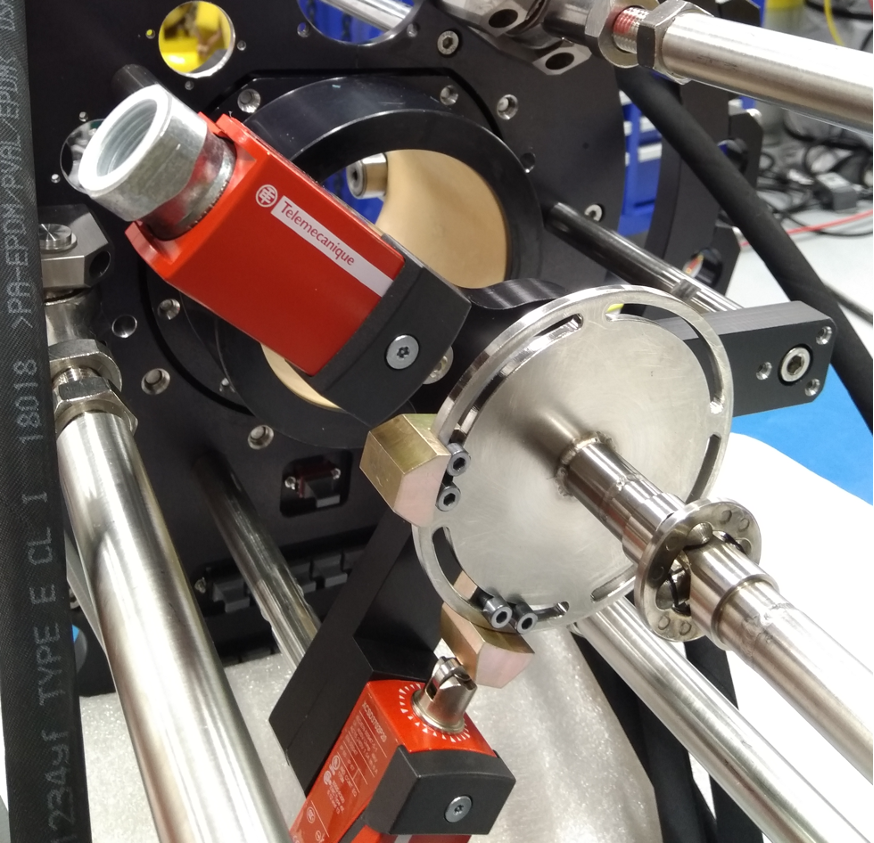
\includegraphics[width=\linewidth]{media/Figure_1.png}
  \caption{Bulkhead Plate with Limit Switches}
  \label{fig:Figure_1}
\end{figure}

\subsection{Objective}

The objective of this characterization is to find the allowable position
range of the positive and negative limit switches and provide a
recommendation of where they should be positioned. This requires finding
the exact position that the limit switches are currently activated,
finding the back off distance required to release the limit switches,
and finding the maximum distance for the CCW and Camera Rotator to come
to a complete stop after activating the limit switches.

\subsection{Requirements}

The following are the relevant requirements for the synchronous motion
between the CCW and the Camera Rotator.

\underline{\citeds{LTS-103}}

\begin{itemize}
\item
  3.10.13 MCS Camera Cable Wrap Positioning Command

  \begin{itemize}
  \item
    \textbf{Specification:} The camera cable wrap shall be slaved to the
    camera rotator.
  \end{itemize}
\end{itemize}

\underline{\citeds{LTS-218}}

\begin{itemize}
\item
  3.3.7 Rotation Drive Synchronization with Camera Rotator

  \begin{itemize}
  \item
    \textbf{Specification:} During slewing and tracking, the camera
    cable wrap rotation shall remain synchronized with the camera
    rotator to better than 2.2 degrees. An absolute rotation sensing
    encoder shall be incorporated on the rotation drive unit to provide
    position feedback to the telescope control system (TCS).
  \end{itemize}
\item
  3.3.8.1 Slewing Velocity Range

  \begin{itemize}
  \item
    \textbf{Specification:} The rotation drive unit shall be able to
    reach any velocity between 0 and 3.5deg/sec with a goal of
    5.25deg/sec in both rotation directions.
  \end{itemize}
\item
  3.16 Safety Pull Cord

  \begin{itemize}
  \item
    \textbf{Specification}: The functionality of the safety pull-cord
    has been replaced by limit switches now specified in \citeds{LTS-156}.
  \end{itemize}
\item
  3.3.1 Rotation Range

  \begin{itemize}
  \item
    \textbf{Specification:} The camera cable wrap shall be designed to rotate
    over a 180 degree operational range (+/- 90 degrees either side of
    centered position). This 180 degree range must be achievable without
    exceeding any software limit, limit switch or hard stop,
    consequently, an additional 8 degrees (+/-4) is required to
    accommodate these items. The software limits shall limit the motion
    to the 180 degree range. The limit switches shall stop the motion
    within 2 degrees of meeting this maximum operational range. The hard
    stops shall stop the motion within another 2 degrees of the limit
    switches.
  \end{itemize}
\end{itemize}

\underline{\citeds{LTS-156}}

\begin{itemize}
\item
  The limits shall be adjusted to nominally stop rotation for any twist
  between the bulkhead plate and the wobble plate greater than +/- 3.5
  degrees with adjustment range from 2.5 degrees to 5 degrees.
\item
  The limit switch shall be tested over the range of travel of the
  wobble plate as specified below.

  \begin{itemize}
  \item
    The wobble plate radial motion is +/- 110mm.
  \item
    The wobble plate tilt about its center is +/- 3 degrees.
  \item
    The wobble plate Z motion is +/- 15mm.
  \end{itemize}
\end{itemize}

\underline{\citeds{LTS-206}}

\begin{itemize}
\item
  3.4.5.1 Rotator Slewing Velocity Range

  \begin{itemize}
  \item
    \textbf{Specification:} During a rotator slew, the Camera Rotator
    shall be able to reach any velocity between 0 and 3.5deg/sec with a
    goal of 5.25deg/sec in both rotation directions.
  \end{itemize}
\item
  3.4.4 Rotator Rotation Range

  \begin{itemize}
  \item
    \textbf{Specification:} The Camera Rotator shall be designed to
    rotate over a 180 degree operational range (+/-90 degrees TBR). This
    range must be achievable without reaching any software limit, limit
    switch or hard stop. The limit switches shall stop the motion within
    2 degrees of meeting this maximum operational range. The hard stops
    shall be within another 2 degrees of the limit switches.
  \end{itemize}
\end{itemize}

\underline{\citeds{LSE-80}}

\begin{itemize}
\item
  CA-TS-MEC-ICD-0058 Maximum Allowed Camera Motion at Bulkhead Plate

  \begin{itemize}
  \item
    \textbf{Specification:} The telescope shall ensure that the maximum
    transverse and axial motions of the back end of the camera utility
    trunk are no larger than \textbf{UTradialMotion} transverse,
    \textbf{UTaxialMotion} axial load, and \textbf{UTrotMotion} angular
    rotation around a radial line.
  \item
    UTrotMotion = 5 degrees
  \end{itemize}
\end{itemize}

\section{Characterization Tasks}\label{sec:Characterization Tasks}

The following sections define the tasks that were performed, the details of
how they were performed, and the results of the task. Due to ComCam being installed,
we will only be performing the characterization with the design velocities.
We do not have any data showing what the emergency stopping maximum deceleration and
jerk values are with a representative load on the camera rotator.
We also do not have a transfer function for the forces from the camera rotator to ComCam.
In order to avoid any issues due to these uncertainties we first performed some initial checks using
the camera rotator at 1 deg/s, then 2 deg/s, and finally the design velocity of 3.5 deg/s.
While doing the consecutive runs into the positive and negative limit switches with the
Rotator we noticed that there was a lot of energy being released when we released the brakes to the
point that it was shaking the table next to the Camera Cart. Due to this rapid engagement and
disengagement of the brakes we decided to limit the number of runs to 5 for each limit switch.


\subsection{Positive Limit Switch Activation Location}\label{sec:Positive Activation}

To determine the exact location that the cam activates the positive
limit switch we moved the CCW slowly and in small increments to find
where the interlock was activated. We moved the CCW at a velocity of 0.1
deg/s and in 0.05 deg increments. This was only performed with the CCW
as it should not matter which system is used to activate the limit
switches at this low velocity and increments.

The positive limit switch was activated at \textbf{+2.80 deg}.

\subsection{Positive Limit Switch Release Location}

The operational process of releasing the interlock is to use the CCW GUI to override the interlock
and then use the jog button to move the CCW in the opposite direction from the limit switch.
The jog function has a max velocity of 0.8 deg/s and can be further reduced using the GUI.
To determine where the positive limit switch is released, we first moved
the CCW slowly and in small jog increments to find where the interlock was
released. We moved the CCW at a velocity of 0.1 deg/s and in approximately 0.05 deg
increments. Next, we moved in a single set of jogs in the releasing direction to find where the limit switch
is released which is a real-world way that we would release the interlock. At these small
distances using the jog functionality, the velocity does not really have much of an impact.
This was only performed with the CCW because the CCW is defined to be the system used to
release the limit switch.

The positive limit switch was released at \textbf{+2.6 deg}.

\subsection{Positive Limit Switch CCW Stopping Distance}

To determine the CCW stopping distance for the design velocity after
activating the positive limit switch we moved the CCW in the positive
direction with enough distance to reach a velocity of 3.5 deg/s before
activating the limit switch. This was repeated 5 times. To
calculate the stopping distance after activation we subtracted the
activation location determined in Section 3.1 from the position the CCW
came to a complete stop.

The maximum stopping distance after activating the positive limit switch
was found to be \textbf{0.47 deg}. See Appendix \ref{sec:data} for the data points
and Appendix \ref{sec:efd} for the EFD data.

\subsection{Positive Limit Switch Camera Rotator Stopping Distance}

To determine the Rotator stopping distance for the design velocity after
activating the positive limit switch we moved the Rotator in the
negative direction with enough distance to reach a velocity of 3.5 deg/s
before activating the limit switch. Since we defined the positive limit
switch to be the limit switch that is activated by the CCW moving in the
positive direction this correlates to the Rotator moving in the negative
direction. This was repeated 5 times. To calculate the stopping
distance after activation we subtracted the activation location
determined in Section \ref{sec:Positive Activation} from the position the Rotator came to a
complete stop.

The maximum stopping distance after activating the positive limit switch
was found to be \textbf{0.69 deg}. See Appendix \ref{sec:data} for the data points
and Appendix \ref{sec:efd} for the EFD data.

\subsection{Negative Limit Switch Activation Location}\label{sec:Negative Activation}

To determine the exact location that the cam activates the negative
limit switch we moved the CCW slowly and in small increments to find
where the interlock was activated. We moved the CCW at a velocity of 0.1
deg/s and in 0.05 deg increments.

The negative limit switch was activated at \textbf{-2.75 deg}.

\subsection{Negative Limit Switch Release Location}

The operational process of releasing the interlock is to use the CCW GUI to override the interlock
and then use the jog button to move the CCW in the opposite direction from the limit switch.
The jog function has a max velocity of 0.8 deg/s and can be further reduced using the GUI.
To determine where the negative limit switch is released, we first moved
the CCW slowly and in small jog increments to find where the interlock was
released. We moved the CCW at a velocity of 0.1 deg/s and in approximately 0.05 deg
increments. Next, we moved in a single set of jogs in the releasing direction to find where the limit switch
is released which is a real-world way that we would release the interlock. At these small
distances using the jog functionality, the velocity does not really have much of an impact.
This was only performed with the CCW because the CCW is defined to be the system used to
release the limit switch.

The negative limit switch was released at \textbf{-2.45 deg}.

\subsection{Negative Limit Switch CCW Stopping Distance}

To determine the CCW stopping distance for the design velocity after
activating the negative limit switch we moved the CCW in the negative
direction with enough distance to reach a velocity of 3.5 deg/s before
activating the limit switch. This was repeated 5 times. To
calculate the stopping distance after activation we subtracted the
activation location determined in Section 3.6 from the position the CCW
came to a complete stop.

The maximum stopping distance after activating the negative limit switch
was found to be \textbf{0.27 deg}. See Appendix \ref{sec:data} for the data points
and Appendix \ref{sec:efd} for the EFD data.

\subsection{Negative Limit Switch Camera Rotator Stopping Distance}

To determine the Rotator stopping distance for the design velocity after
activating the negative limit switch we moved the Rotator in the
positive direction with enough distance to reach a velocity of 3.5 deg/s
before activating the limit switch. Since we defined the negative limit
switch to be the limit switch that is activated by the CCW moving in the
negative direction this correlates to the Rotator moving in the positive
direction. This was repeated 5 times. To calculate the stopping
distance after activation we subtracted the activation location
determined in Section \ref{sec:Negative Activation} from the position the Rotator came to a
complete stop.

The maximum stopping distance after activating the negative limit switch
was found to be \textbf{0.44 deg}. See Appendix \ref{sec:data} for the data points
and Appendix \ref{sec:efd} for the EFD data.

\subsection{Normal Operational Conditions Stopping Distance}

Normal operating conditions for the system is to have the CCW following the motion of Rotator.
To determine what the maximum angular difference the system will experience under
normal operating conditions we reduced the maximum velocity of the CCW to 2.6 deg/s so that the Rotator
will get up to maximum velocity and the CCW will fall behind and the limit switch will be activated
and stop both the CCW and the Rotator. This was repeated 5 times alternating from moving in the
positive direction and negative direction.

The maximum angular distance after activating the limit switch
was found to be \textbf{3.36 deg}. See Appendix \ref{sec:efd} for the EFD data.

\subsection{Software Limit Stopping Distance}

In addition to the hardware limit switches there is also an adjustable software limit for the
following error between the CCW and the Rotator. The Rotator monitors the position of the CCW
and if the following error software limit is reached it will fault the Rotator which will stop it's motion.
The CCW continues it's motion and re-aligns with the Rotator. This task is to verify that if the software
limit is reached that the limit switches will not also be activated. The default software limit is +/- 2.2 degrees.
To determine if this situation occurs we reduced the maximum velocity of the CCW to 2.6 deg/s so that
the Rotator will get up to maximum velocity and the CCW will fall behind and the following error software
limit will be reached. This was repeated 5 times alternating from moving in the positive direction
and negative direction.

After reaching the software limit the limit switches \textbf{TBD}.

\section{Recommendations}

\subsection{Characterization Results}

The tables below provides a summary of the calculations performed on the
data captured to determine the result of the tasks define in Section \ref{sec:Characterization Tasks}.

\begin{table}[h!]
  \begin{center}
    \caption{CCW Positive Limit Switch Characterization Calculation Results}
    \label{tab:table1}
    \begin{tabular}{r|c|r|c|c|c}
    \multicolumn{3}{l|}{\textbf{CCW Positive Limit Switch}} & Avg & Max & Std Dev\\
    \midrule
    Activation location: & 2.8 & & & & \\
    Release location: & 2.6 & 3.5 deg/s stopping location: & 3.246 & 3.27 & 0.01743 \\
    Incremental delta: & 0.2 & 3.5 deg/s stopping distance: & 0.446 & \textbf{0.47} & \\
    \end{tabular}
  \end{center}
\end{table}

\begin{table}[h!]
  \begin{center}
    \caption{CCW Negative Limit Switch Characterization Calculation Results}
    \label{tab:table2}
    \begin{tabular}{r|c|r|c|c|c}
    \multicolumn{3}{l|}{\textbf{CCW Negative Limit Switch}} & Avg & Max & Std Dev\\
    \midrule
    Activation location: & -2.75 & & & & \\
    Release location: & -2.45 & 3.5 deg/s stopping location: & -3.006 & -3.02 & 0.01019 \\
    Incremental delta: & 0.3 & 3.5 deg/s stopping distance: & -0.256 & \textbf{0.27} & \\
    \end{tabular}
  \end{center}
\end{table}

\begin{table}[h!]
  \begin{center}
    \caption{Rotator Positive Limit Switch Characterization Calculation Results}
    \label{tab:table3}
    \begin{tabular}{r|c|r|c|c|c}
    \multicolumn{3}{l|}{\textbf{Rotator Positive Limit Switch}} & Avg & Max & Std Dev\\
    \midrule
    Activation location: & -2.8 & & & & \\
    Release location: & -2.6 & 3.5 deg/s stopping location: & -3.466 & -3.49 & 0.01356 \\
    Incremental delta: & 0.2 & 3.5 deg/s stopping distance: & 0.666 & \textbf{0.69} & \\
    \end{tabular}
  \end{center}
\end{table}

\begin{table}[h!]
  \begin{center}
    \caption{Rotator Negative Limit Switch Characterization Calculation Results}
    \label{tab:table4}
    \begin{tabular}{r|c|r|c|c|c}
    \multicolumn{3}{l|}{\textbf{Rotator Negative Limit Switch}} & Avg & Max & Std Dev\\
    \midrule
    Activation location: & 2.75 & & & & \\
    Release location: & 2.45 & 3.5 deg/s stopping location: & 3.144 & 3.19 & 0.02576 \\
    Incremental delta: & 0.3 & 3.5 deg/s stopping distance: & 0.394 & \textbf{0.44} & \\
    \end{tabular}
  \end{center}
\end{table}

\subsection{Limit Switch Activation Location Recommendation}

The \citeds{LSE-80} requirement for the angular rotation between the bulkhead plate and the wobble plate is
5 degrees so that should be the minimum slack in the utility lines and
the maximum angular rotation between the CCW and the Rotator after
activating the limit switch and coming to a complete stop.

Based on the requirements and characterization of the limit switches we
recommend that the limit switch activation location should be
\textbf{+/- 2.75 deg}. We recommend that the cams that activate the limit switches should remain where
they currently are located at -2.75 and 2.8 since the maximum angular distance between the CCW and
Rotator is currently less than 3.5 degrees which is well below the design limit of 5.0 degrees and
there are no issues releasing the interlock or activating the limit switch after reaching the
following error software limit \textbf{TBR}.

\appendix
% Include all the relevant bib files.
% https://lsst-texmf.lsst.io/lsstdoc.html#bibliographies
\section{References} \label{sec:bib}
\renewcommand{\refname}{} % Suppress default Bibliography section
\bibliography{local,lsst,refs_ads,refs,books}

% Make sure lsst-texmf/bin/generateAcronyms.py is in your path
\section{Acronyms} \label{sec:acronyms}
\input{acronyms.tex}
% If you want glossary uncomment below -- comment out the two lines above
%\printglossaries

\section{Data Points} \label{sec:data}
\subsection{CCW Positive Limit Switch Data Points}
\begin{figure}[h!]
  \centering
  \begin{subfigure}{0.49\linewidth}
    \centering
    \begin{tabular}{c|c}
    \multicolumn{2}{c}{\textbf{3.5 Deg/s}}\\
    \midrule
    Run & Location \\
    1 & 3.24 \\
    2 & 3.27 \\
    3 & 3.24 \\
    4 & 3.26 \\
    5 & 3.22 \\
    \midrule
    Avg & \textbf{3.246} \\
    Max & \textbf{3.27} \\
    Std Dev & \textbf{0.0174356} \\
    \bottomrule
    \end{tabular}
  \end{subfigure}
  \begin{subfigure}{0.49\linewidth}
    \centering
    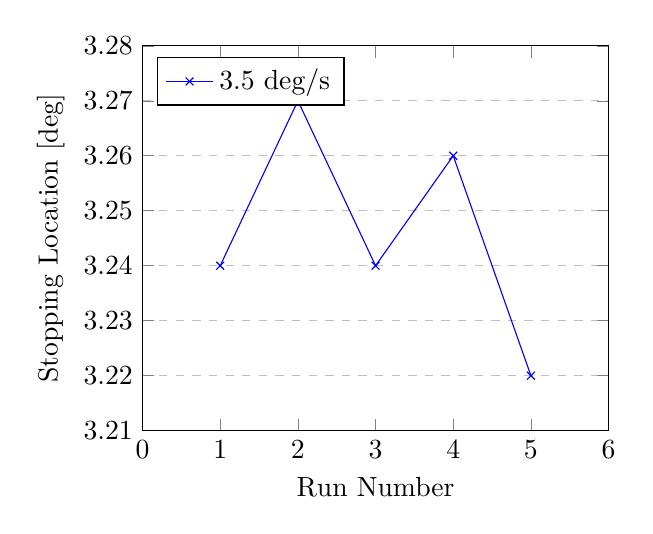
\begin{tikzpicture}
    \begin{axis}[
    xlabel={Run Number},
    ylabel={Stopping Location [deg]},
    xmin=0, xmax=6,
    ymin=3.21, ymax=3.28,
    xtick={0,1,2,3,4,5,6},
    ytick={0,3.21,3.22,3.23,3.24,3.25,3.26,3.27,3.28},
    legend pos=north west,
    ymajorgrids=true,
    grid style=dashed,
    ]
    \addplot[
    color=blue,
    mark=x,
    ]
    coordinates {
    (1,3.24)(2,3.27)(3,3.24)(4,3.26)(5,3.22)};
    \legend{3.5 deg/s}
    \end{axis}
    \end{tikzpicture}
  \end{subfigure}
  \caption{CCW Positive Limit Switch Data Points}
  \label{tab:table5}
\end{figure}

\subsection{CCW Negative Limit Switch Data Points}
\begin{figure}[h!]
  \centering
  \begin{subfigure}{0.49\linewidth}
    \centering
    \begin{tabular}{c|c}
    \multicolumn{2}{c}{\textbf{3.5 Deg/s}}\\
    \midrule
    Run & Location \\
    1 & -3.00 \\
    2 & -3.01 \\
    3 & -3.02 \\
    4 & -3.01 \\
    5 & -2.99 \\
    \midrule
    Avg & \textbf{-3.006} \\
    Max & \textbf{-3.02} \\
    Std Dev & \textbf{0.01019804} \\
    \bottomrule
    \end{tabular}
  \end{subfigure}
  \begin{subfigure}{0.49\linewidth}
    \centering
    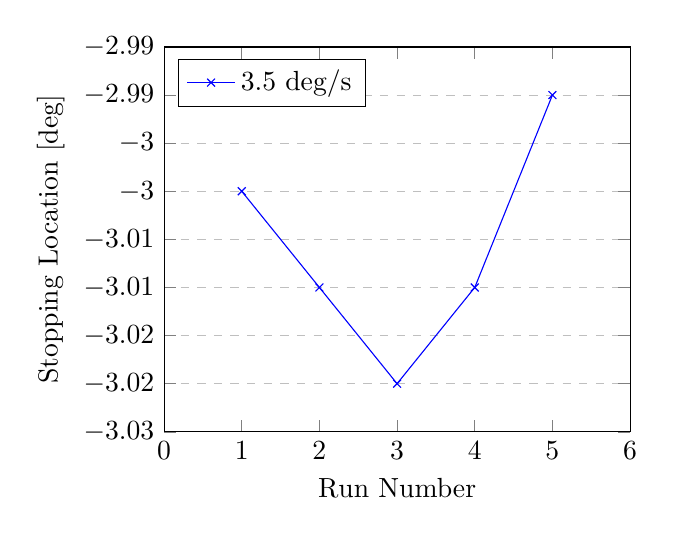
\begin{tikzpicture}
    \begin{axis}[
    xlabel={Run Number},
    ylabel={Stopping Location [deg]},
    xmin=0, xmax=6,
    ymin=-3.025, ymax=-2.985,
    xtick={0,1,2,3,4,5,6},
    ytick={0,-3.025,-3.02,-3.015,-3.01,-3.005,-3,-2.995,-2.99,-2.985},
    legend pos=north west,
    ymajorgrids=true,
    grid style=dashed,
    ]
    \addplot[
    color=blue,
    mark=x,
    ]
    coordinates {
    (1,-3.00)(2,-3.01)(3,-3.02)(4,-3.01)(5,-2.99)};
    \legend{3.5 deg/s}
    \end{axis}
    \end{tikzpicture}
  \end{subfigure}
  \caption{CCW Negative Limit Switch Data Points}
  \label{tab:table6}
\end{figure}
\newpage
\subsection{Rotator Positive Limit Switch Data Points}
\begin{figure}[h!]
  \centering
  \begin{subfigure}{0.49\linewidth}
    \centering
    \begin{tabular}{c|c}
    \multicolumn{2}{c}{\textbf{3.5 Deg/s}}\\
    \midrule
    Run & Location \\
    1 & -3.49 \\
    2 & -3.45 \\
    3 & -3.46 \\
    4 & -3.46 \\
    5 & -3.47 \\
    \midrule
    Avg & \textbf{-3.466} \\
    Max & \textbf{-3.49} \\
    Std Dev & \textbf{0.01356466} \\
    \bottomrule
    \end{tabular}
  \end{subfigure}
  \begin{subfigure}{0.49\linewidth}
    \centering
    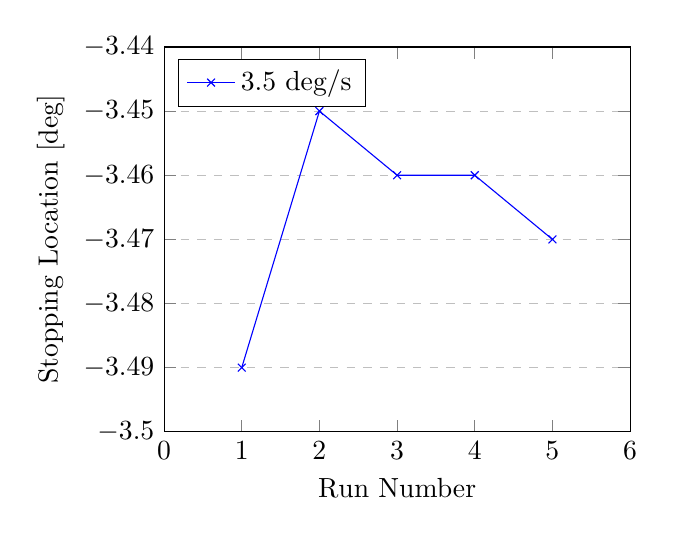
\begin{tikzpicture}
    \begin{axis}[
    xlabel={Run Number},
    ylabel={Stopping Location [deg]},
    xmin=0, xmax=6,
    ymin=-3.5, ymax=-3.44,
    xtick={0,1,2,3,4,5,6},
    ytick={0,-3.5,-3.49,-3.48,-3.47,-3.46,-3.45,-3.44},
    legend pos=north west,
    ymajorgrids=true,
    grid style=dashed,
    ]
    \addplot[
    color=blue,
    mark=x,
    ]
    coordinates {
    (1,-3.49)(2,-3.45)(3,-3.46)(4,-3.46)(5,-3.47)};
    \legend{3.5 deg/s}
    \end{axis}
    \end{tikzpicture}
  \end{subfigure}
  \caption{Rotator Positive Limit Switch Data Points}
  \label{tab:table7}
\end{figure}

\subsection{Rotator Negative Limit Switch Data Points}
\begin{figure}[h!]
  \centering
  \begin{subfigure}{0.49\linewidth}
    \centering
    \begin{tabular}{c|c}
    \multicolumn{2}{c}{\textbf{3.5 Deg/s}}\\
    \midrule
    Run & Location \\
    1 & 3.12 \\
    2 & 3.15 \\
    3 & 3.12 \\
    4 & 3.14 \\
    5 & 3.19 \\
    \midrule
    Avg & \textbf{3.144} \\
    Max & \textbf{3.19} \\
    Std Dev & \textbf{0.0257682} \\
    \bottomrule
    \end{tabular}
  \end{subfigure}
  \begin{subfigure}{0.49\linewidth}
    \centering
    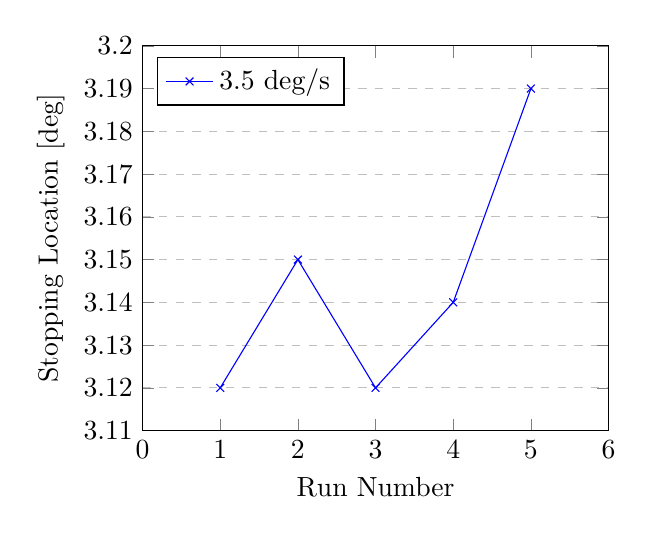
\begin{tikzpicture}
    \begin{axis}[
    xlabel={Run Number},
    ylabel={Stopping Location [deg]},
    xmin=0, xmax=6,
    ymin=3.11, ymax=3.2,
    xtick={0,1,2,3,4,5,6},
    ytick={0,3.11,3.12,3.13,3.14,3.15,3.16,3.17,3.18,3.19,3.2},
    legend pos=north west,
    ymajorgrids=true,
    grid style=dashed,
    ]
    \addplot[
    color=blue,
    mark=x,
    ]
    coordinates {
    (1,3.12)(2,3.15)(3,3.12)(4,3.14)(5,3.19)};
    \legend{3.5 deg/s}
    \end{axis}
    \end{tikzpicture}
  \end{subfigure}
  \caption{Rotator Negative Limit Switch Data Points}
  \label{tab:table8}
\end{figure}
\newpage
\section{EFD Plots} \label{sec:efd}
\subsection{CCW Positive Limit Switch EFD Data}
\begin{figure}
  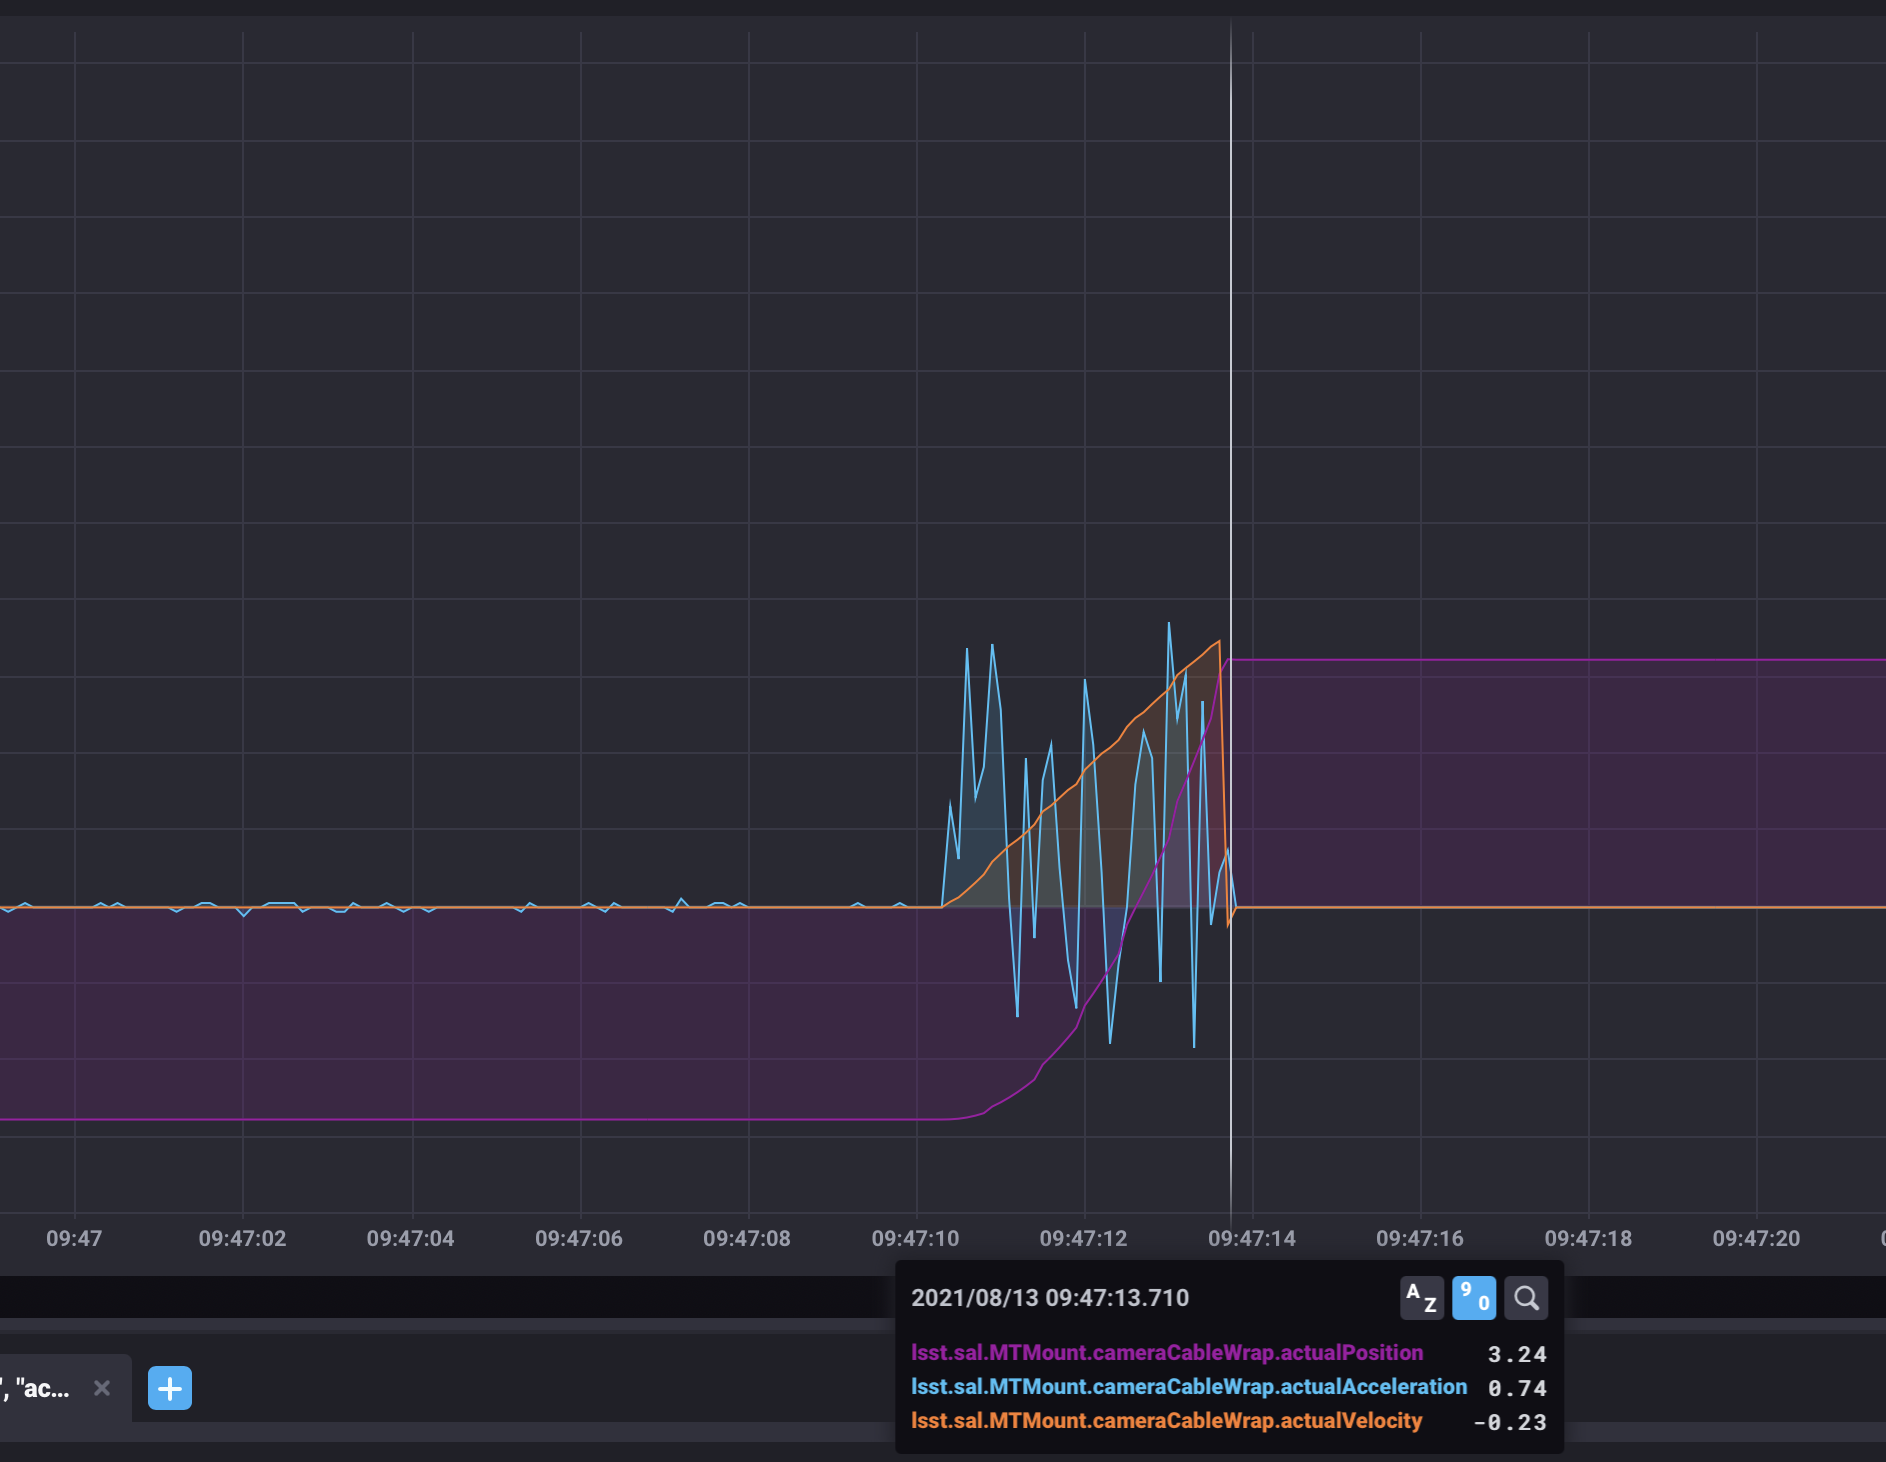
\includegraphics[width=\linewidth]{media/ccw_pos_1.png}
  \caption{CCW\_POS\_RUN\_1}
  \label{fig:CCW_POS_RUN_1}
\end{figure}
\newpage
\begin{figure}
  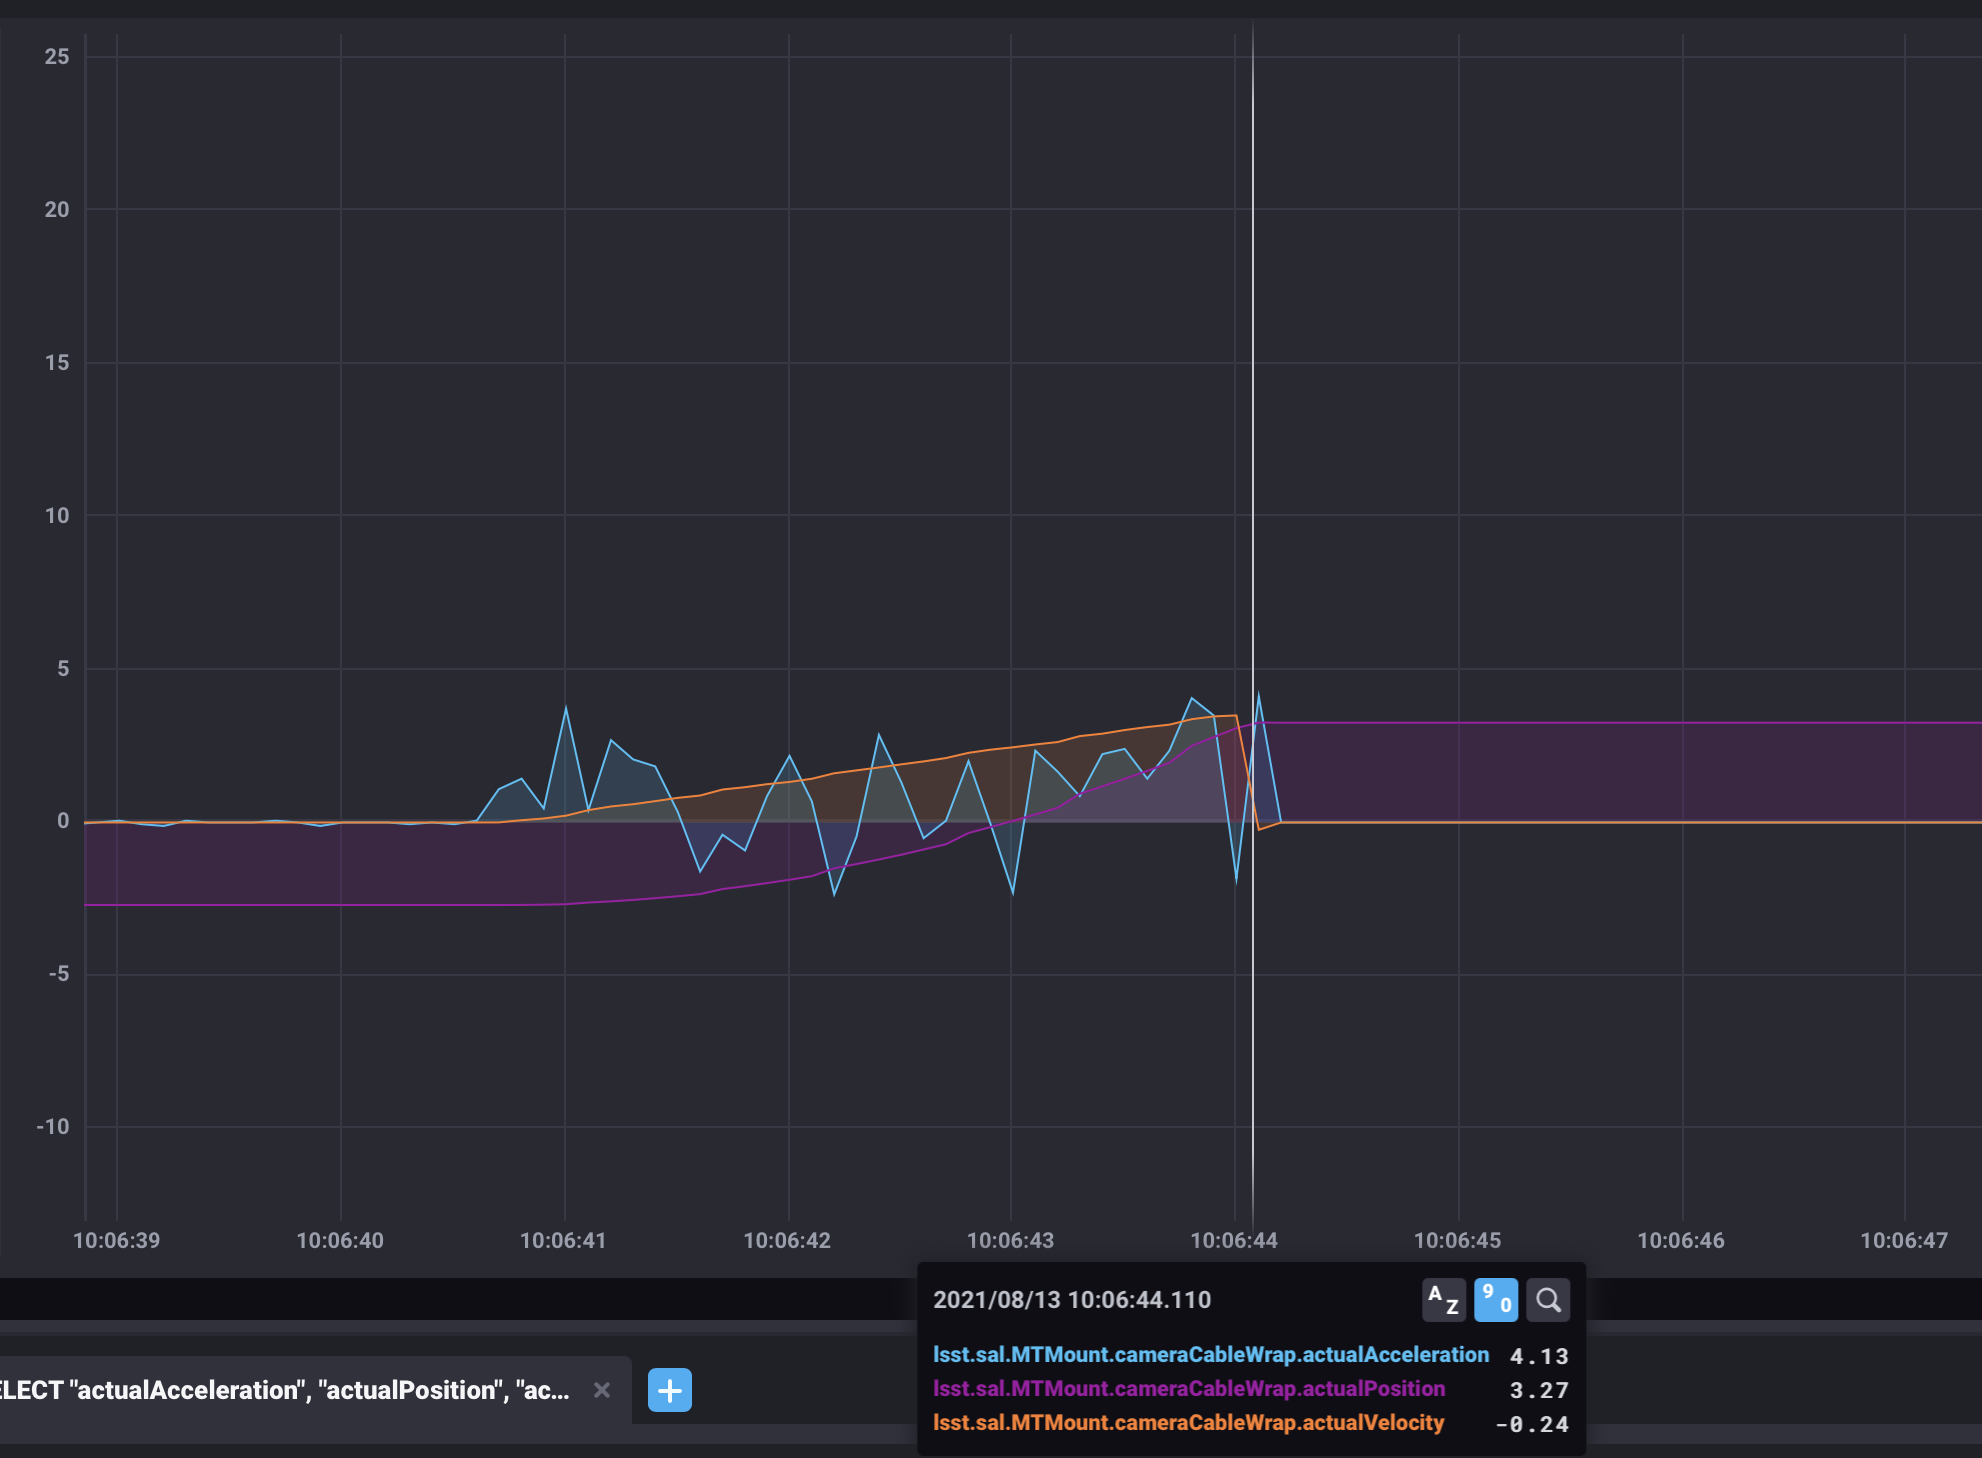
\includegraphics[width=\linewidth]{media/ccw_pos_2.png}
  \caption{CCW\_POS\_RUN\_2}
  \label{fig:CCW_POS_RUN_2}
\end{figure}
\newpage
\begin{figure}
  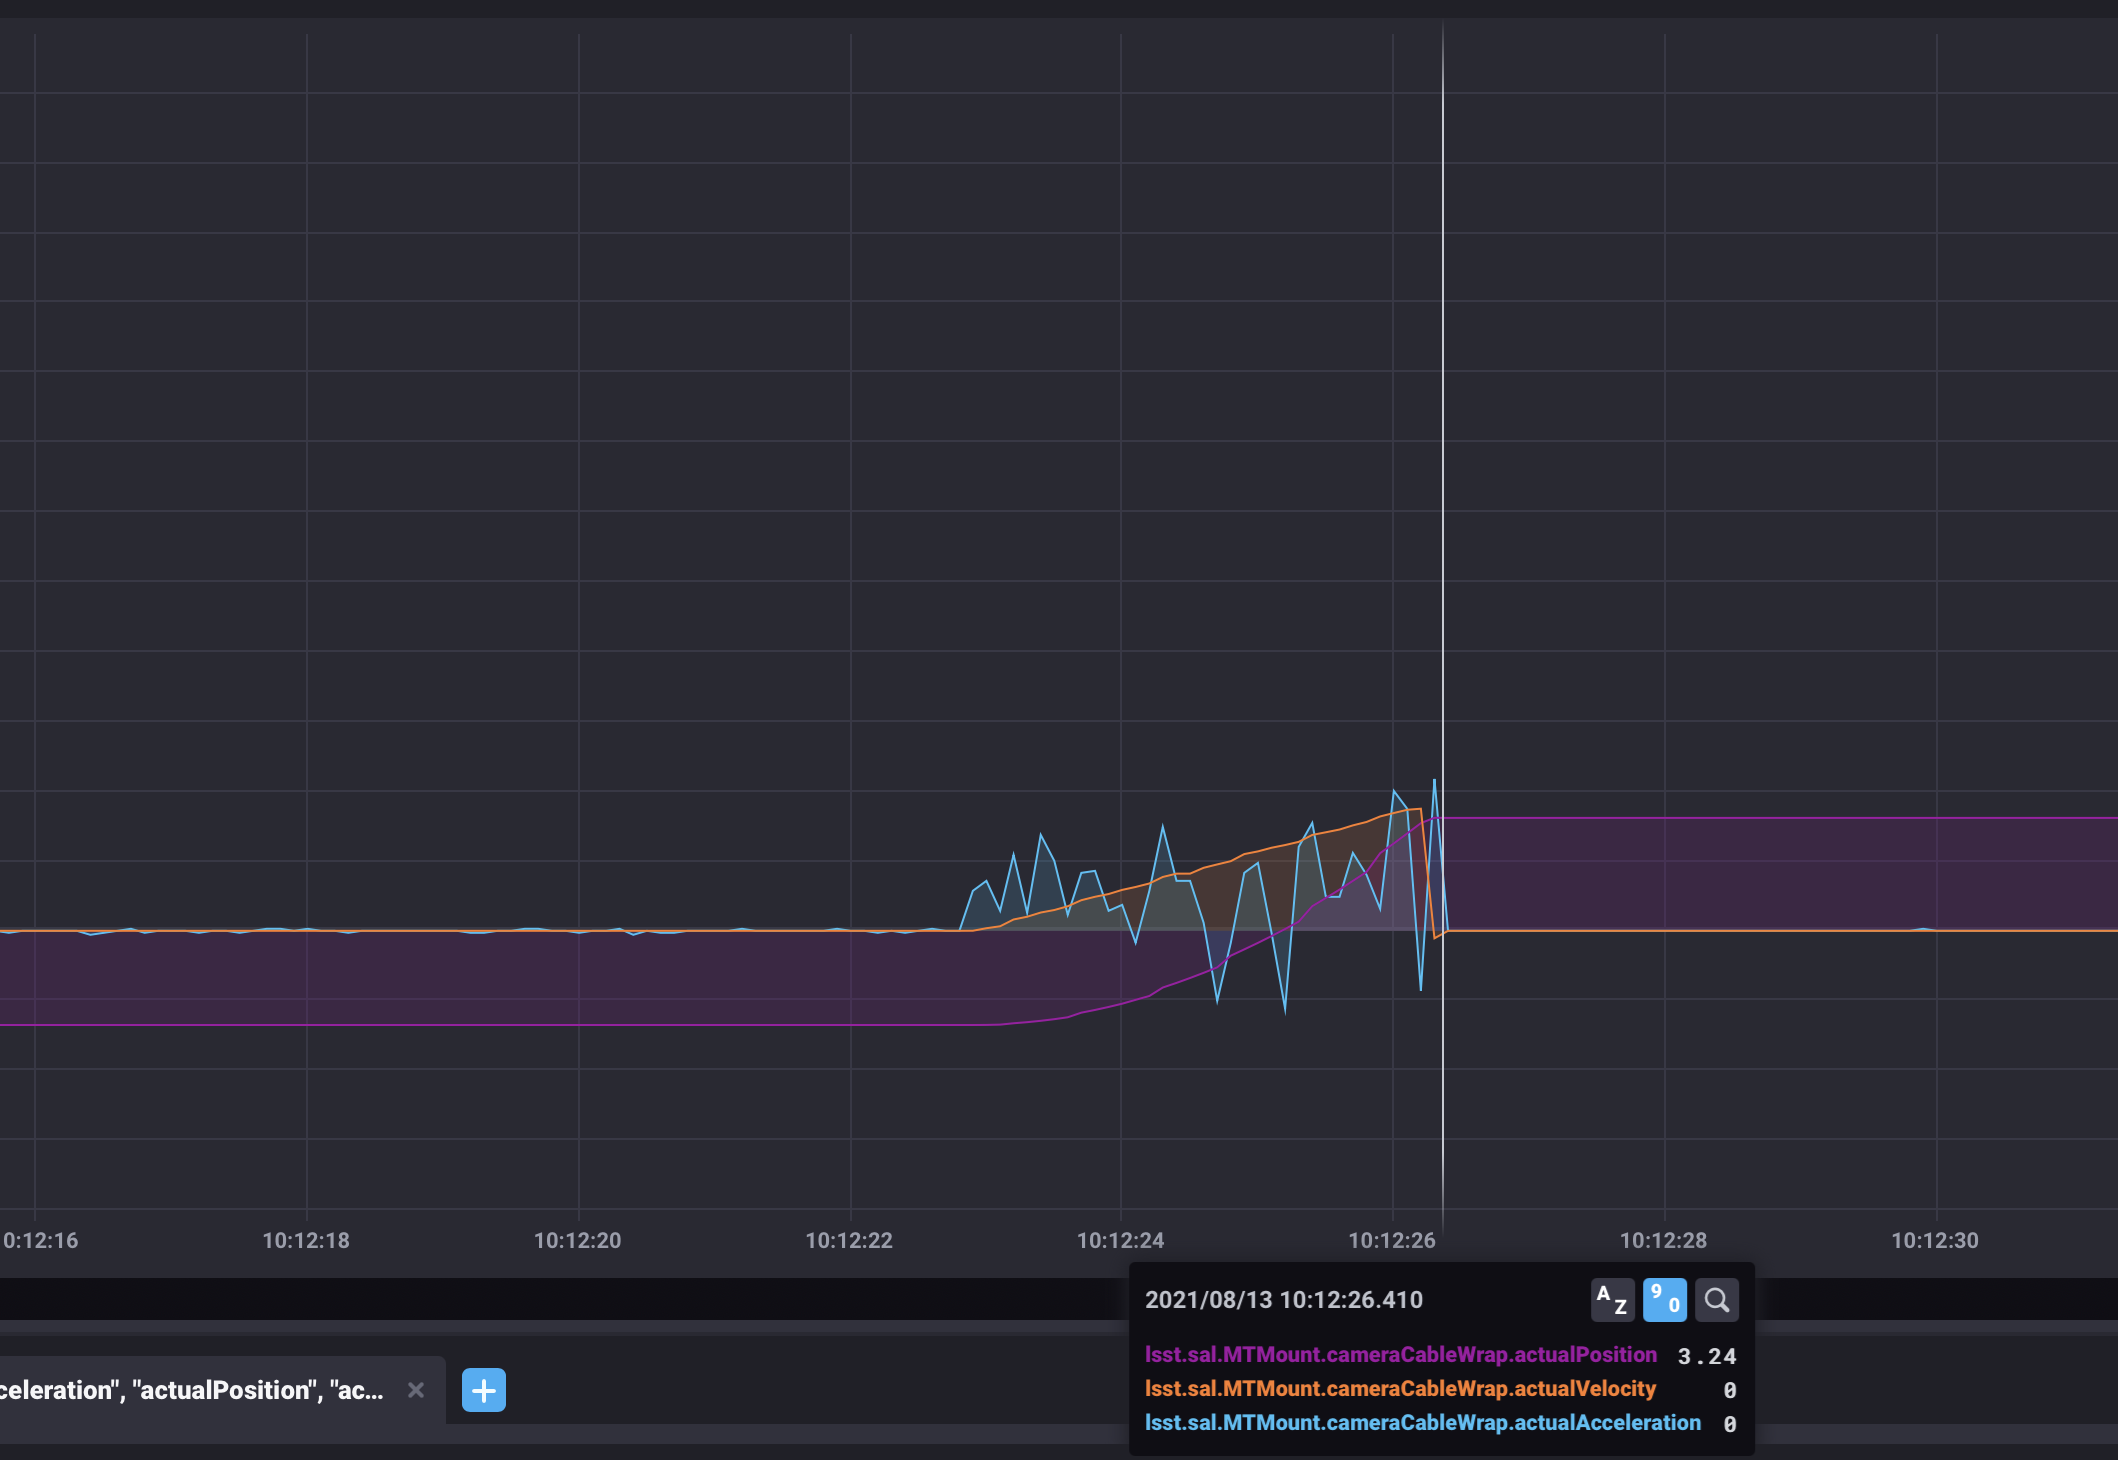
\includegraphics[width=\linewidth]{media/ccw_pos_3.png}
  \caption{CCW\_POS\_RUN\_3}
  \label{fig:CCW_POS_RUN_3}
\end{figure}
\newpage
\begin{figure}
  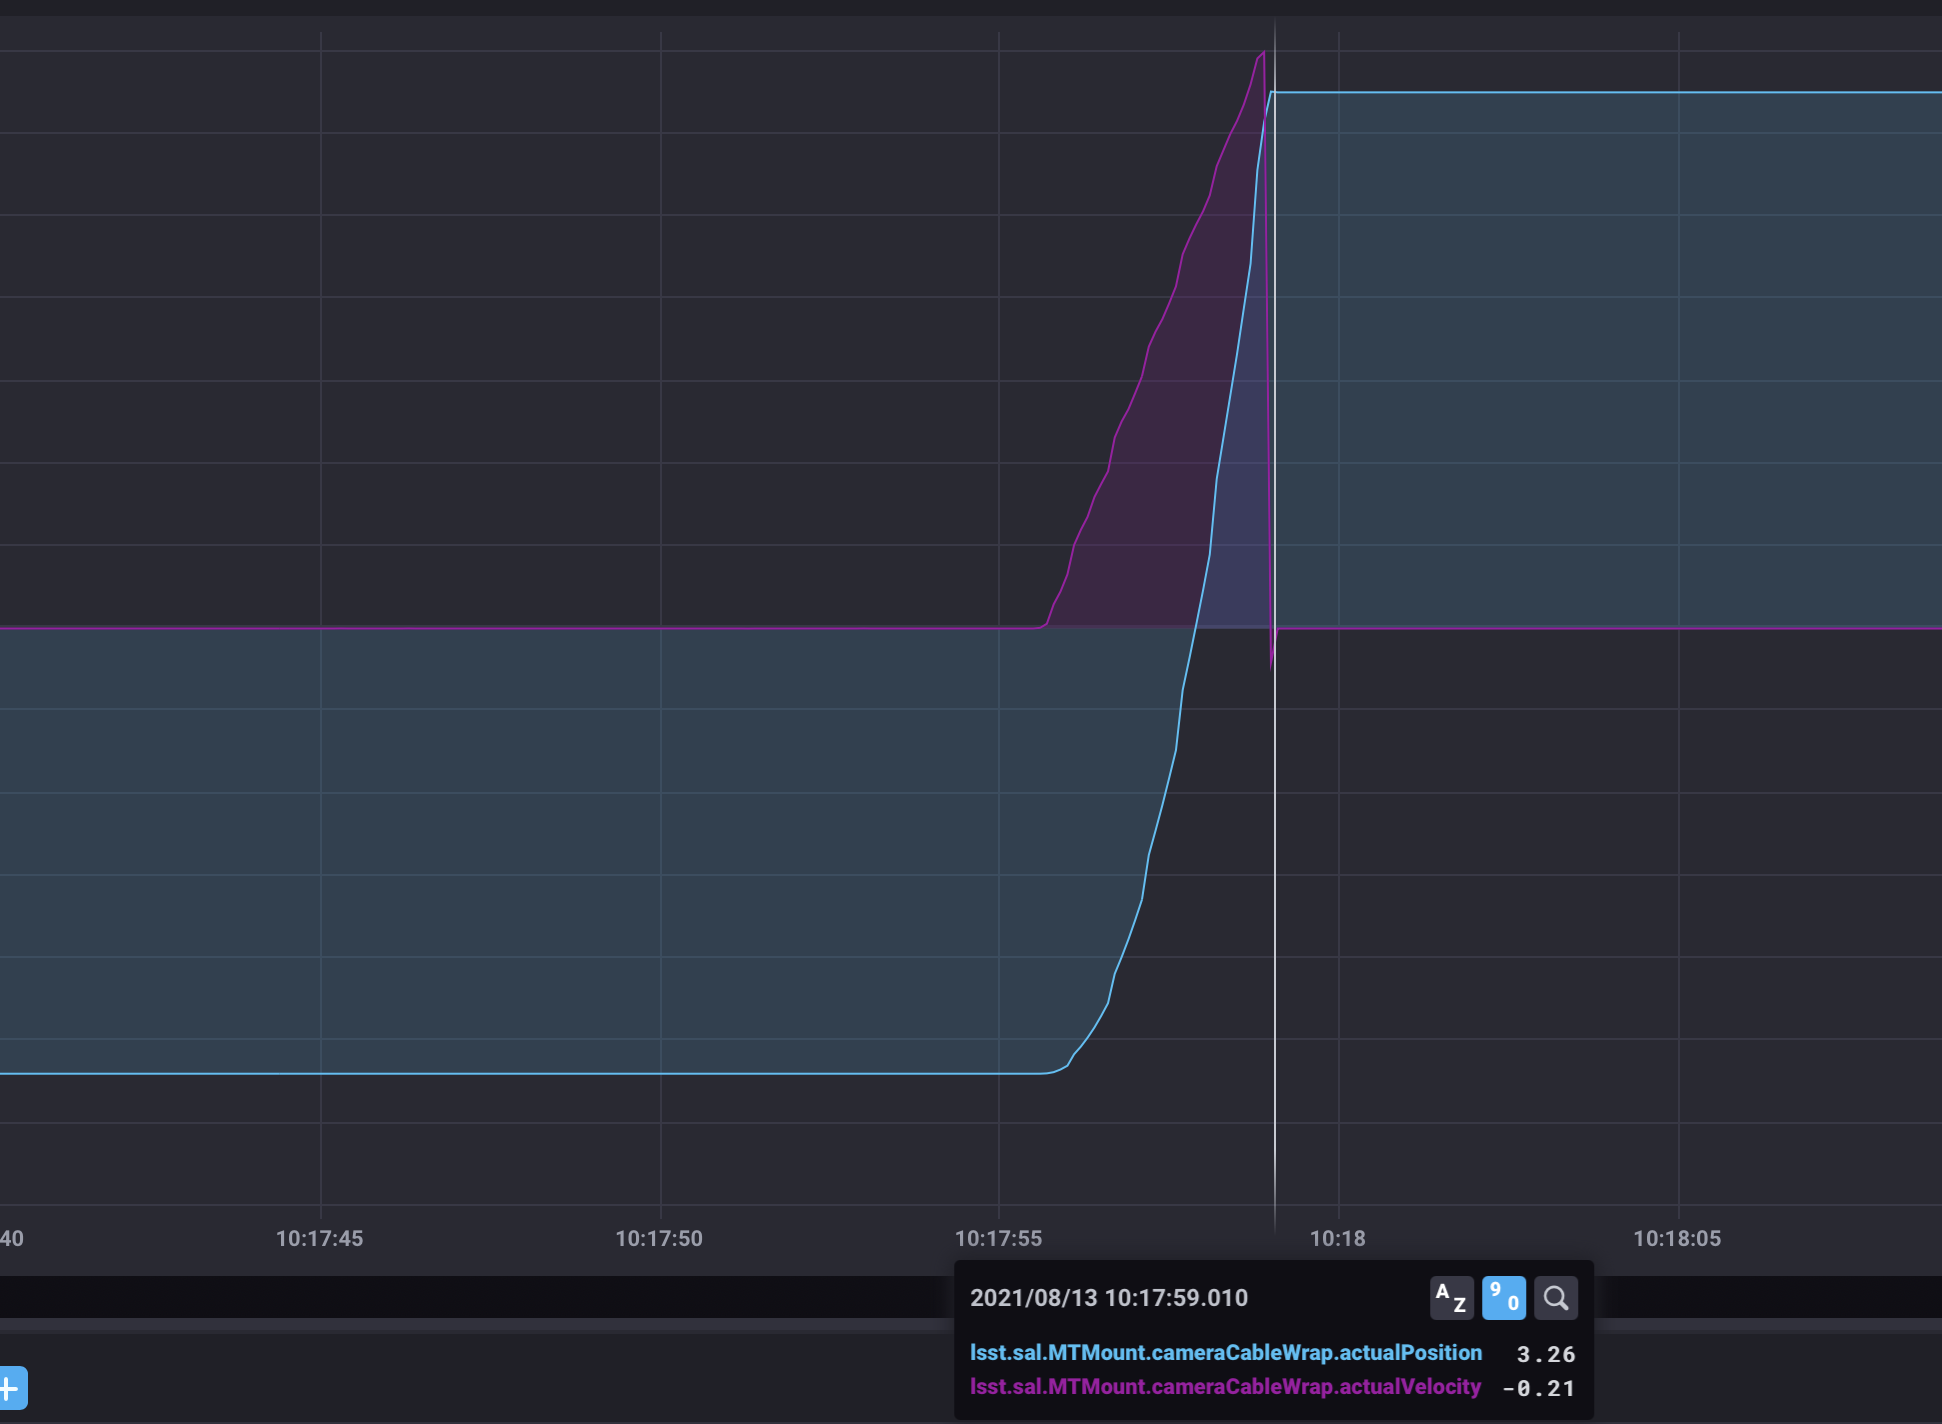
\includegraphics[width=\linewidth]{media/ccw_pos_4.png}
  \caption{CCW\_POS\_RUN\_4}
  \label{fig:CCW_POS_RUN_4}
\end{figure}
\newpage
\begin{figure}
  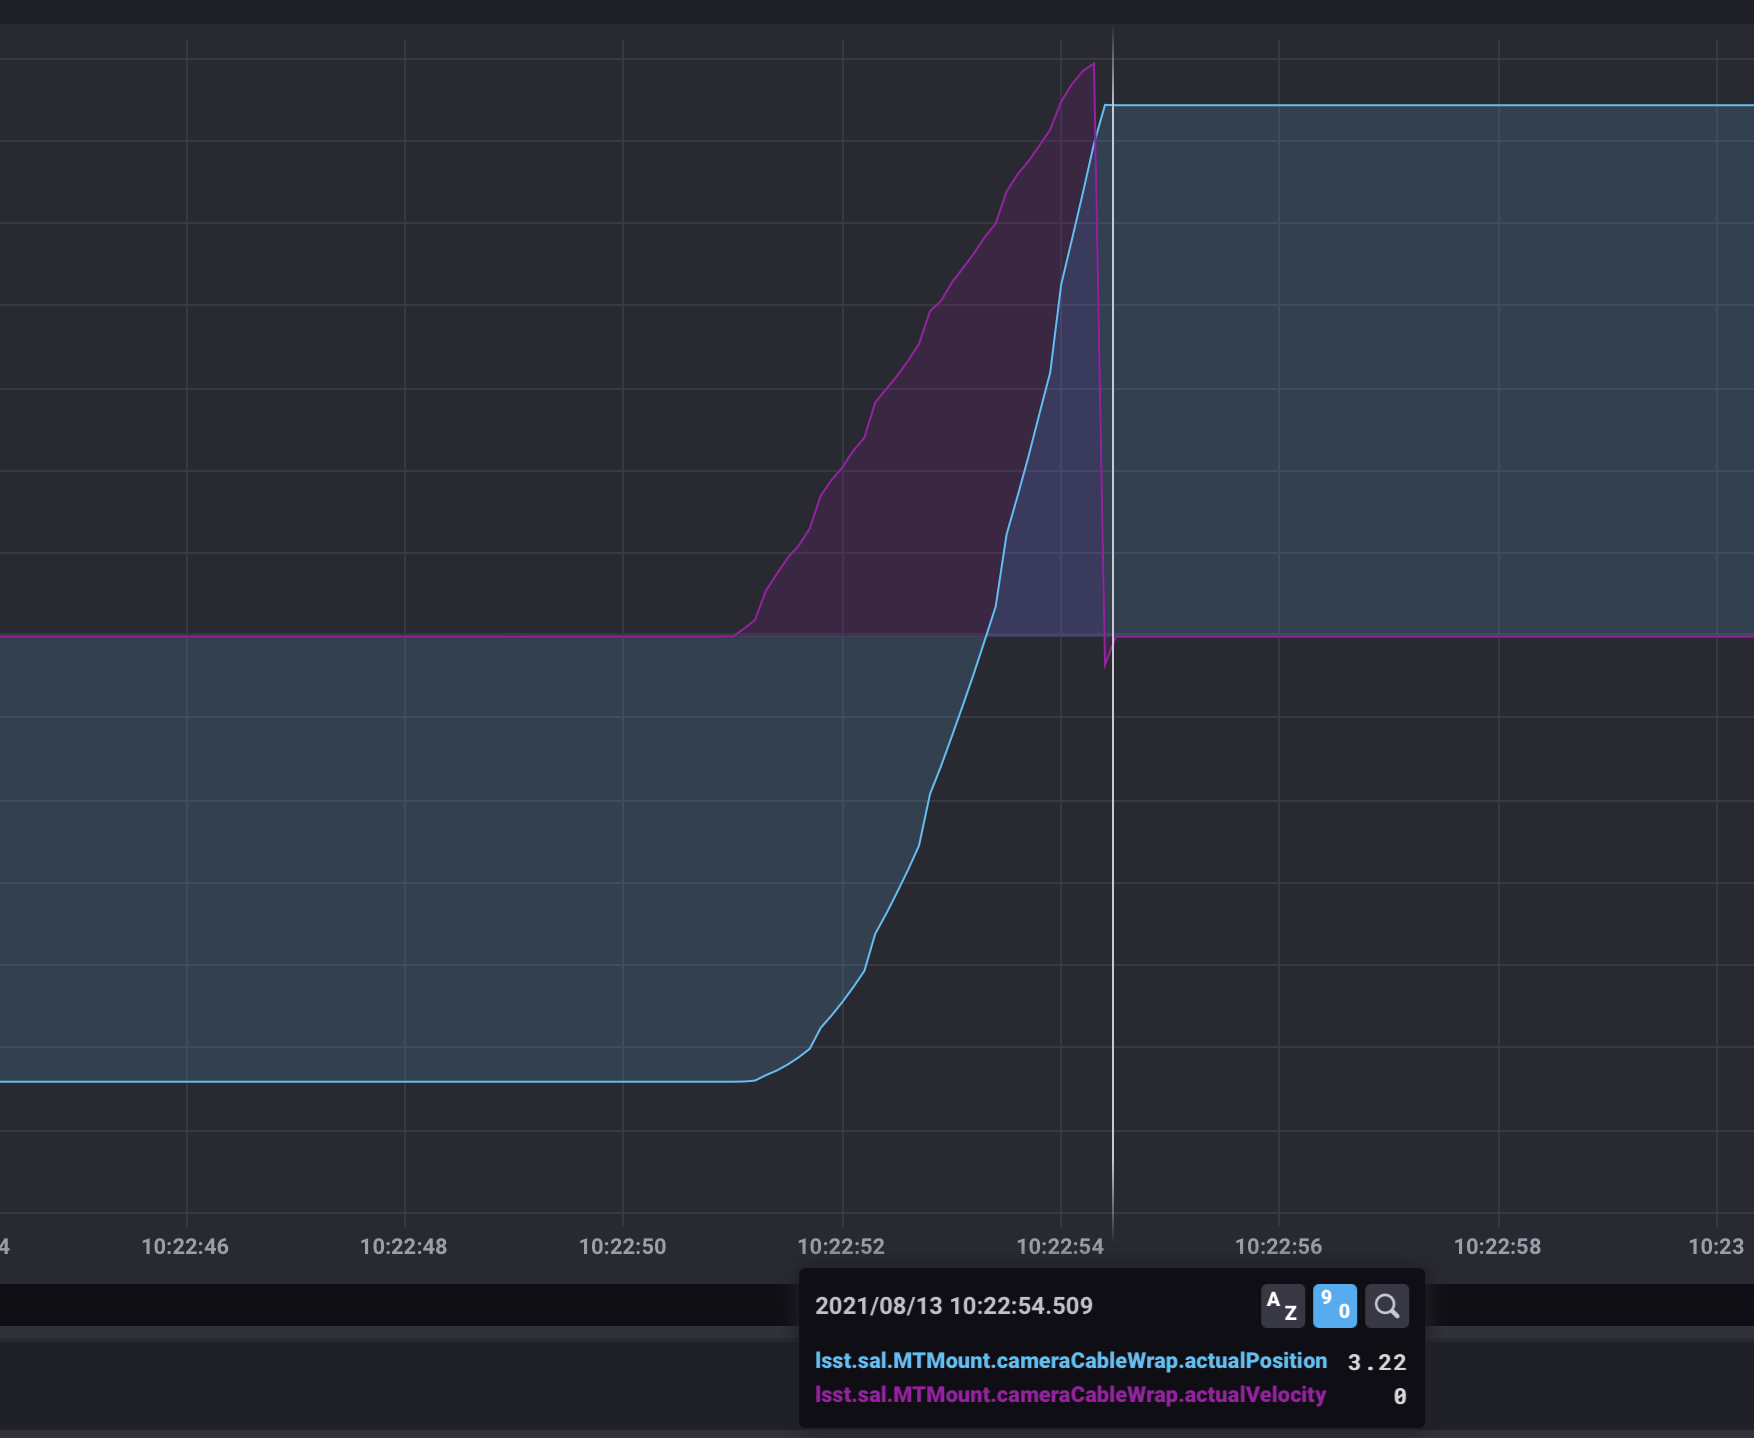
\includegraphics[width=\linewidth]{media/ccw_pos_5.png}
  \caption{CCW\_POS\_RUN\_5}
  \label{fig:CCW_POS_RUN_5}
\end{figure}
\newpage
\subsection{CCW Negative Limit Switch EFD Data}
\begin{figure}
  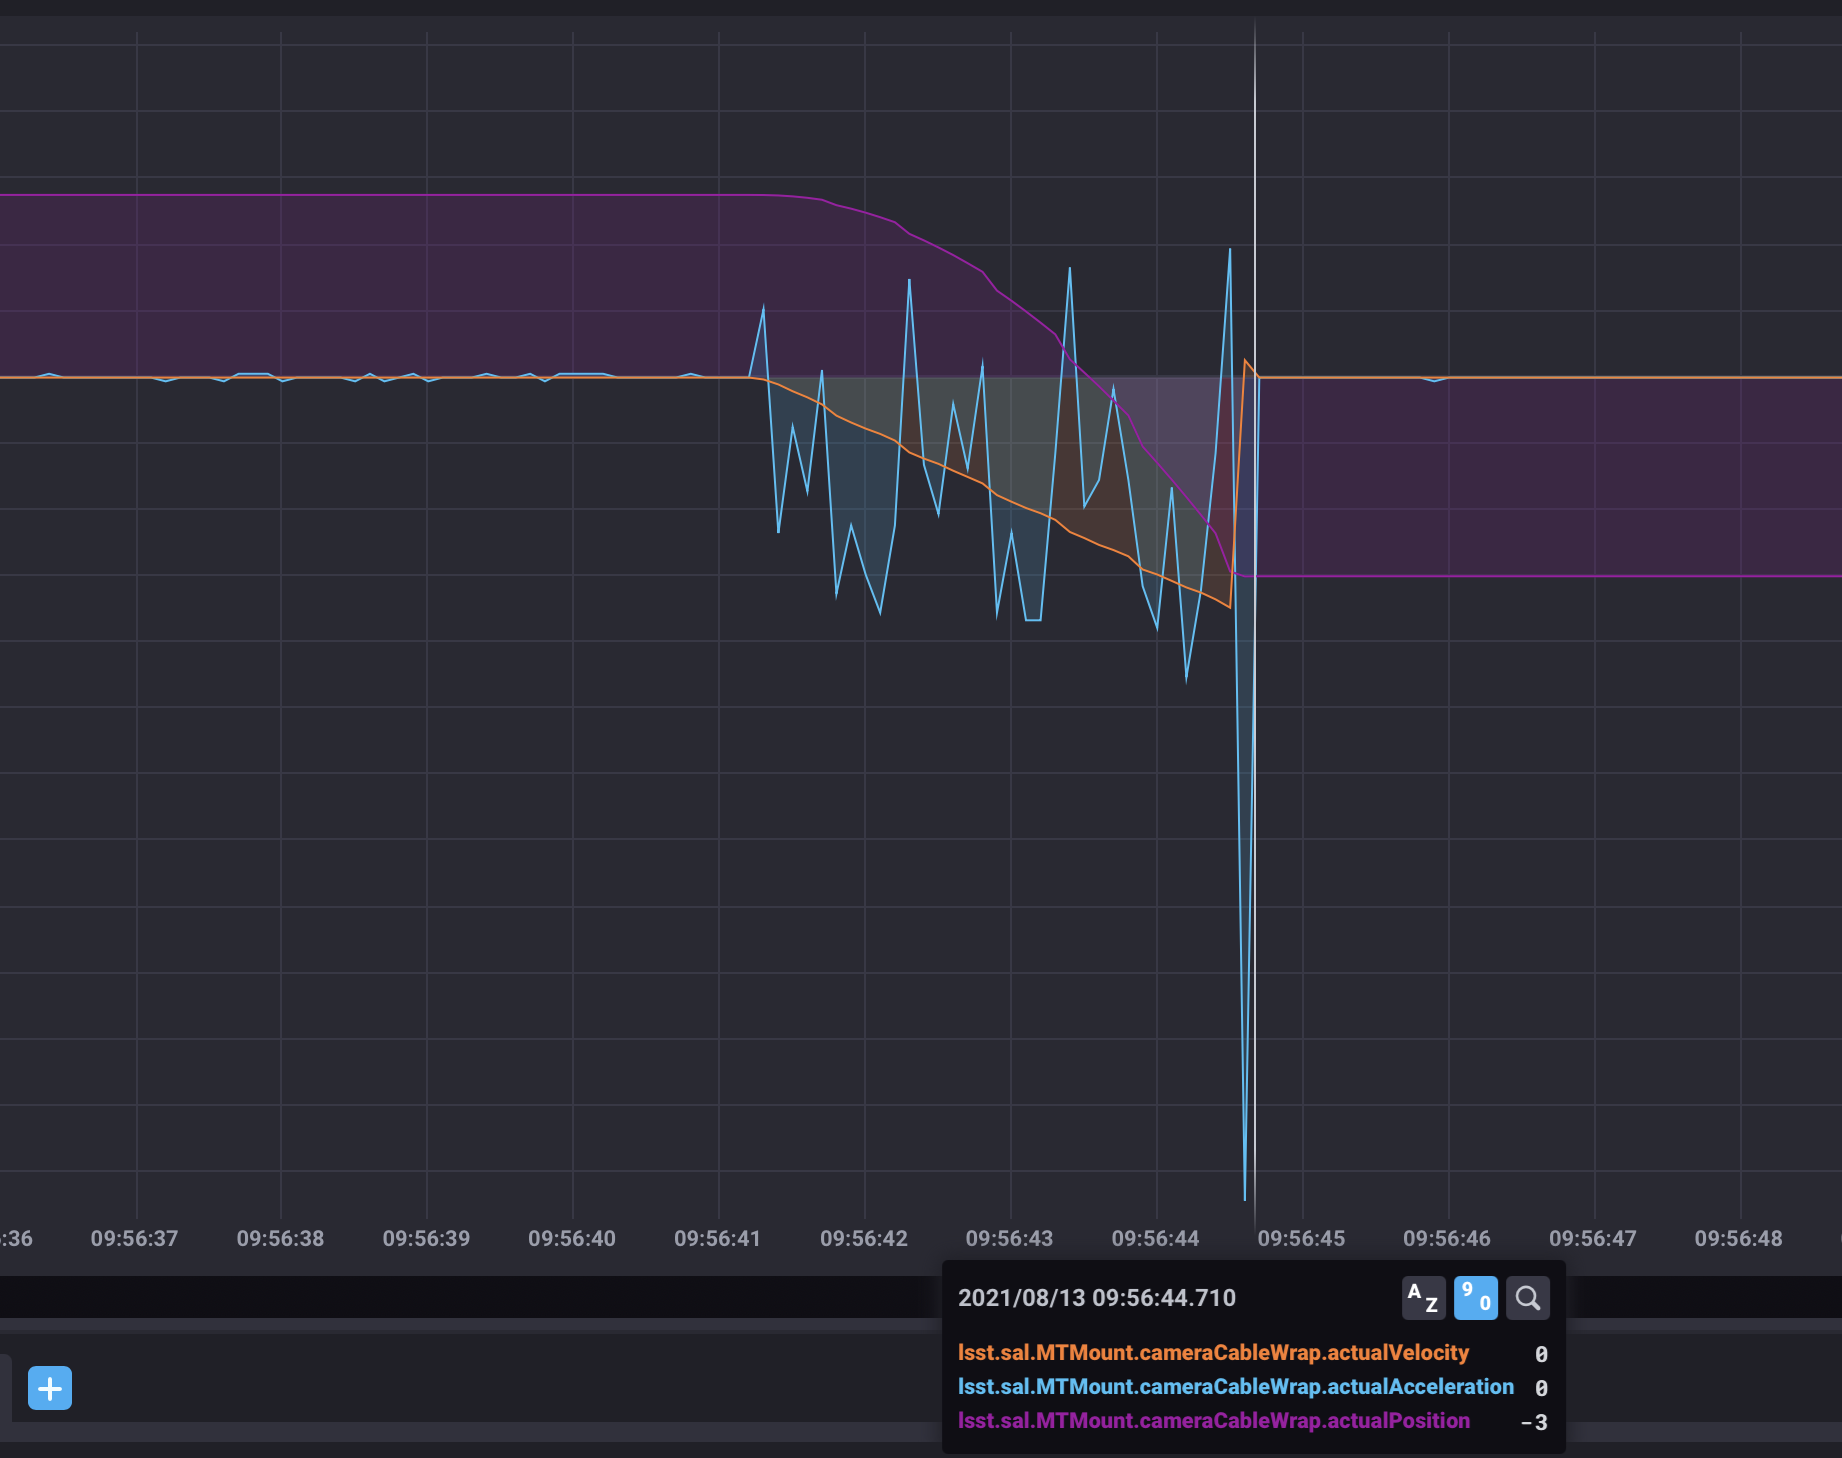
\includegraphics[width=\linewidth]{media/ccw_neg_1.png}
  \caption{CCW\_NEG\_RUN\_1}
  \label{fig:CCW_NEG_RUN_1}
\end{figure}

\begin{figure}
  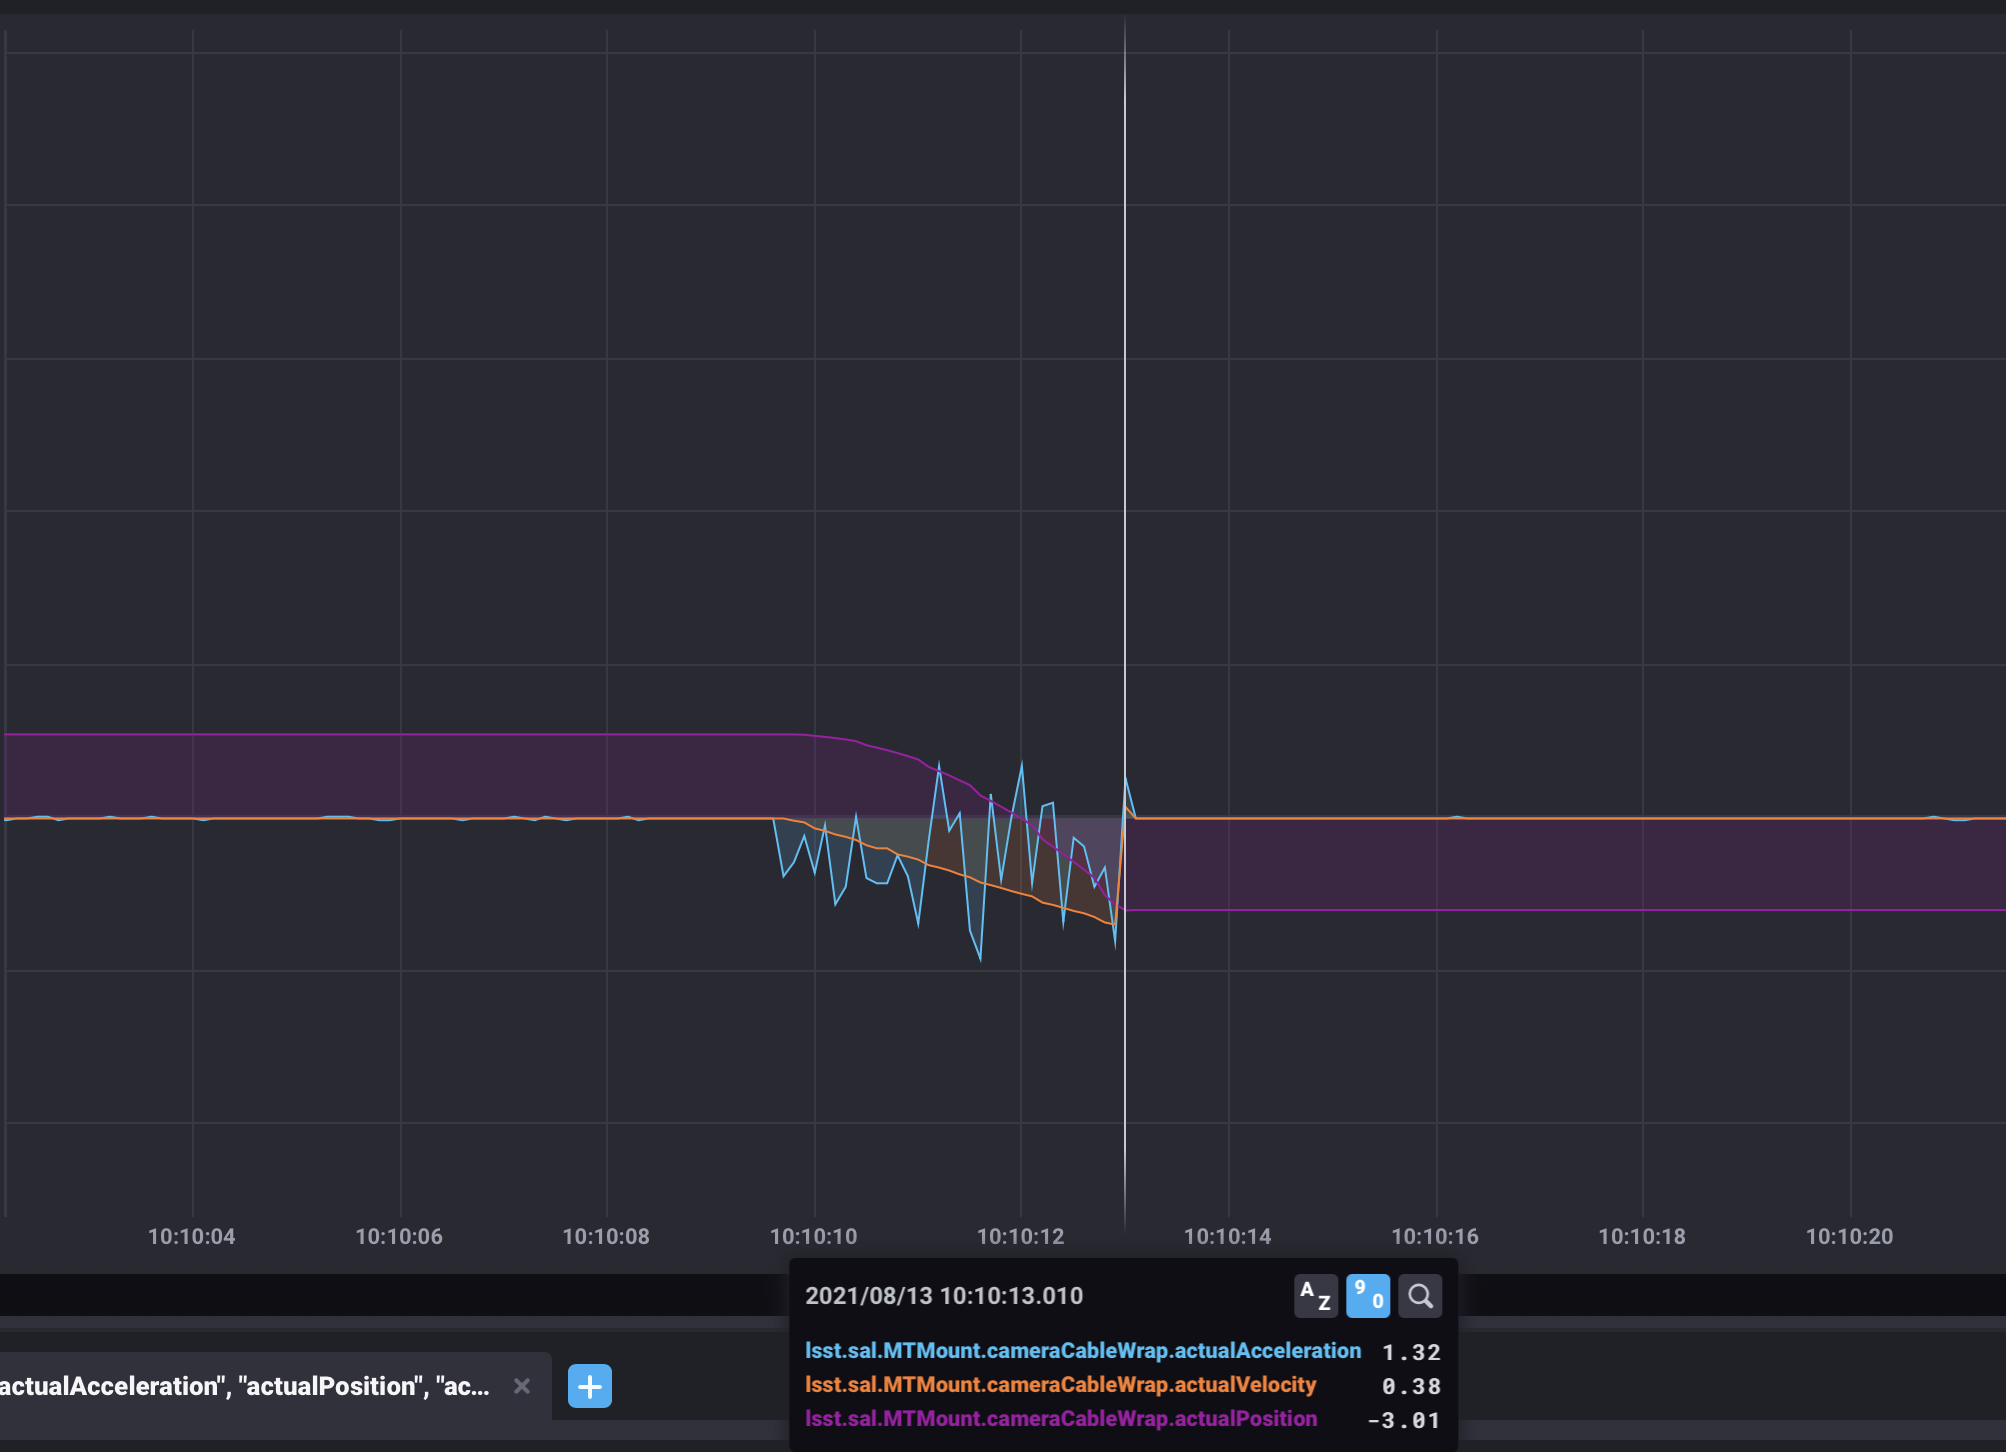
\includegraphics[width=\linewidth]{media/ccw_neg_2.png}
  \caption{CCW\_NEG\_RUN\_2}
  \label{fig:CCW_NEG_RUN_2}
\end{figure}

\begin{figure}
  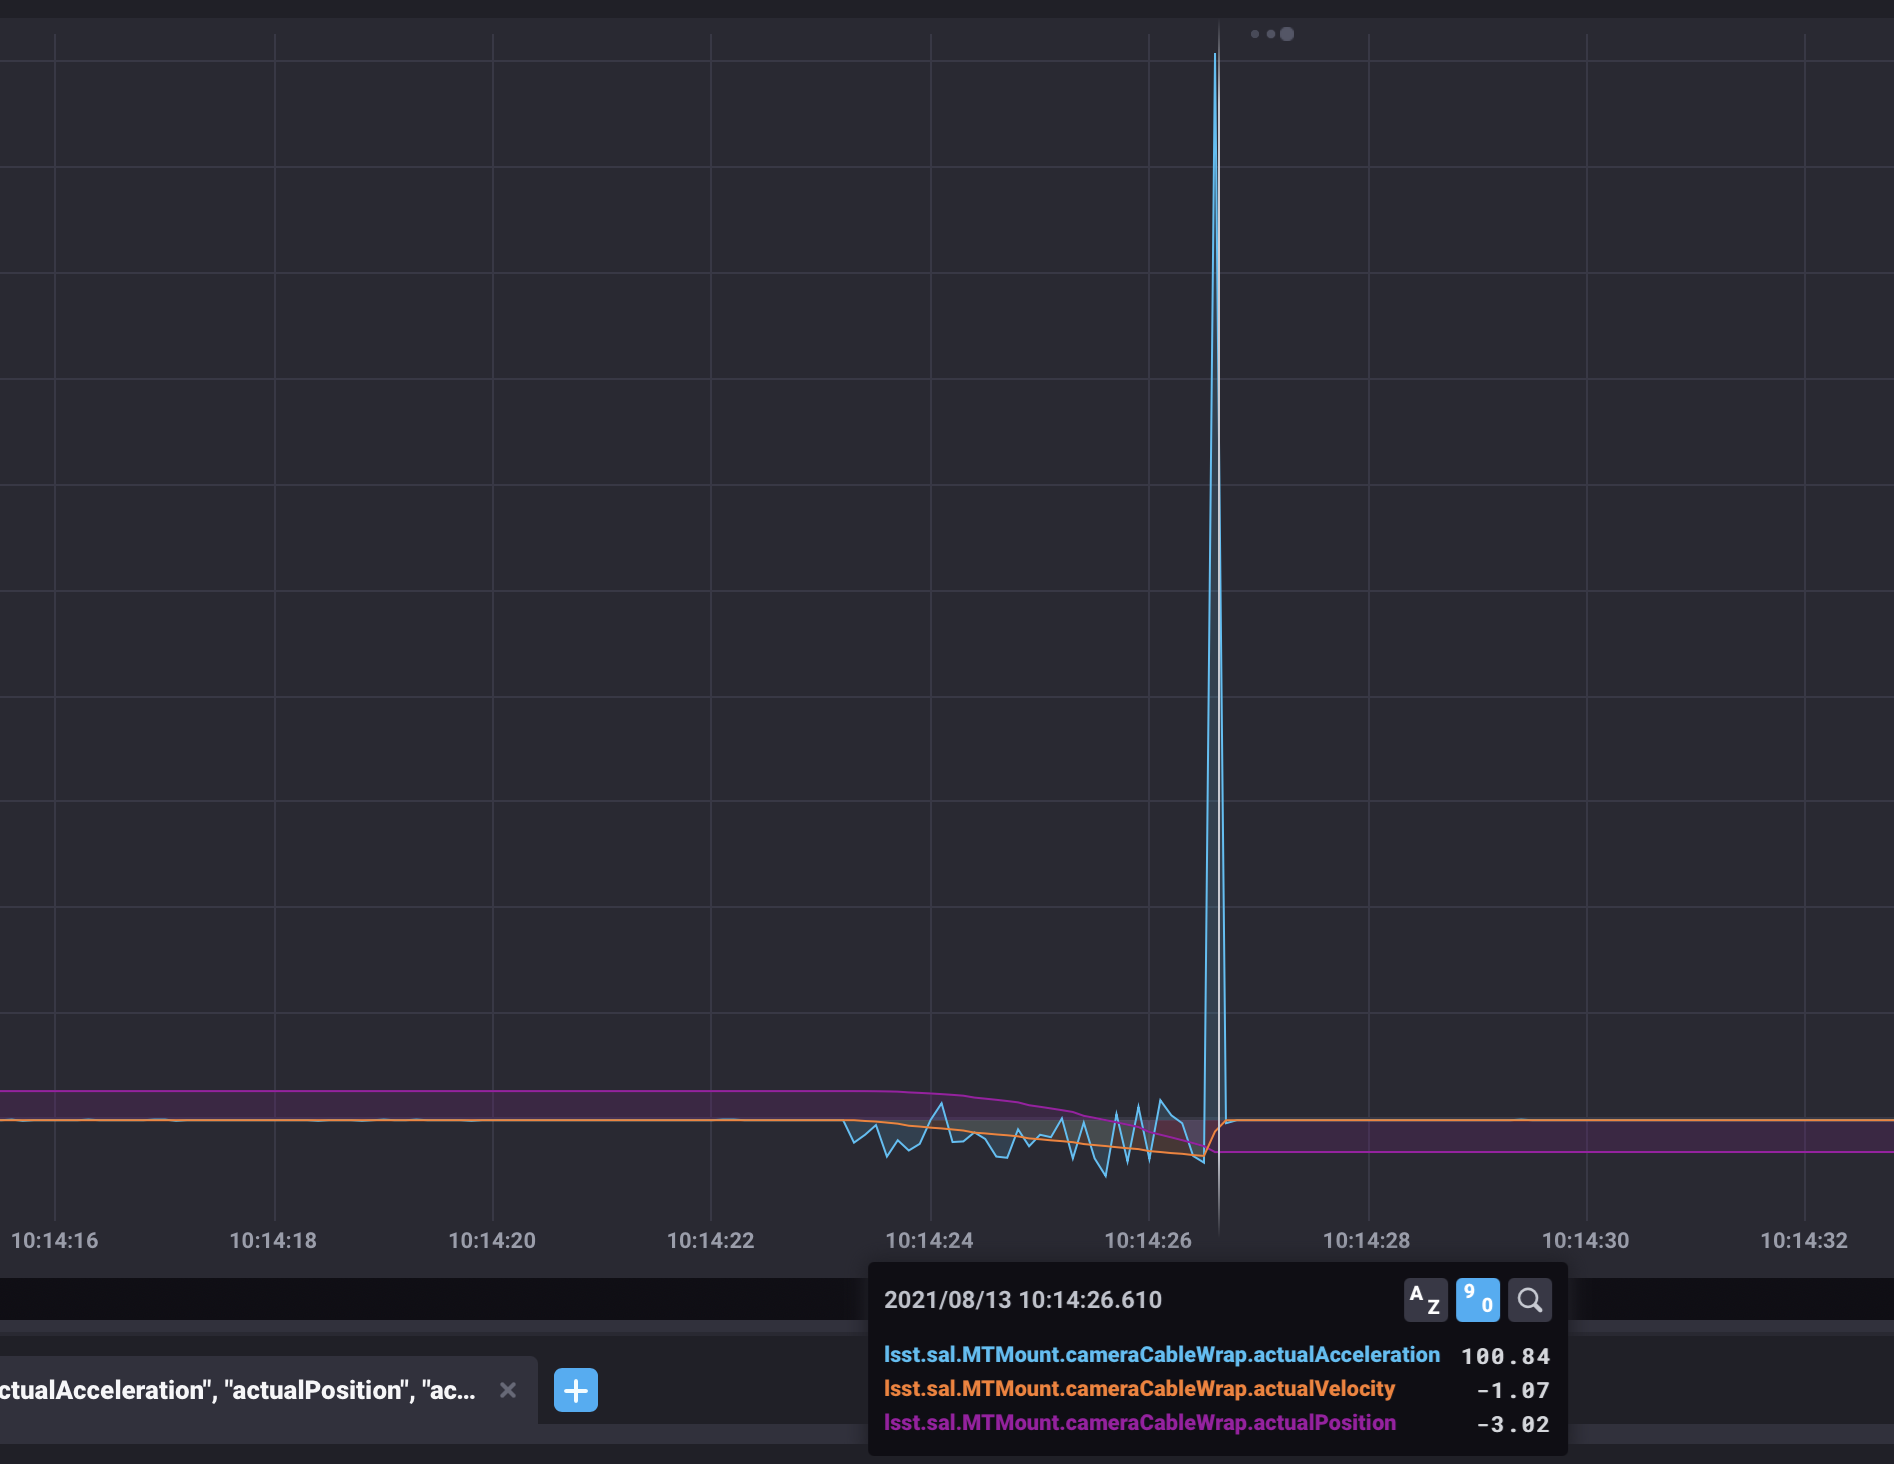
\includegraphics[width=\linewidth]{media/ccw_neg_3.png}
  \caption{CCW\_NEG\_RUN\_3}
  \label{fig:CCW_NEG_RUN_3}
\end{figure}

\begin{figure}
  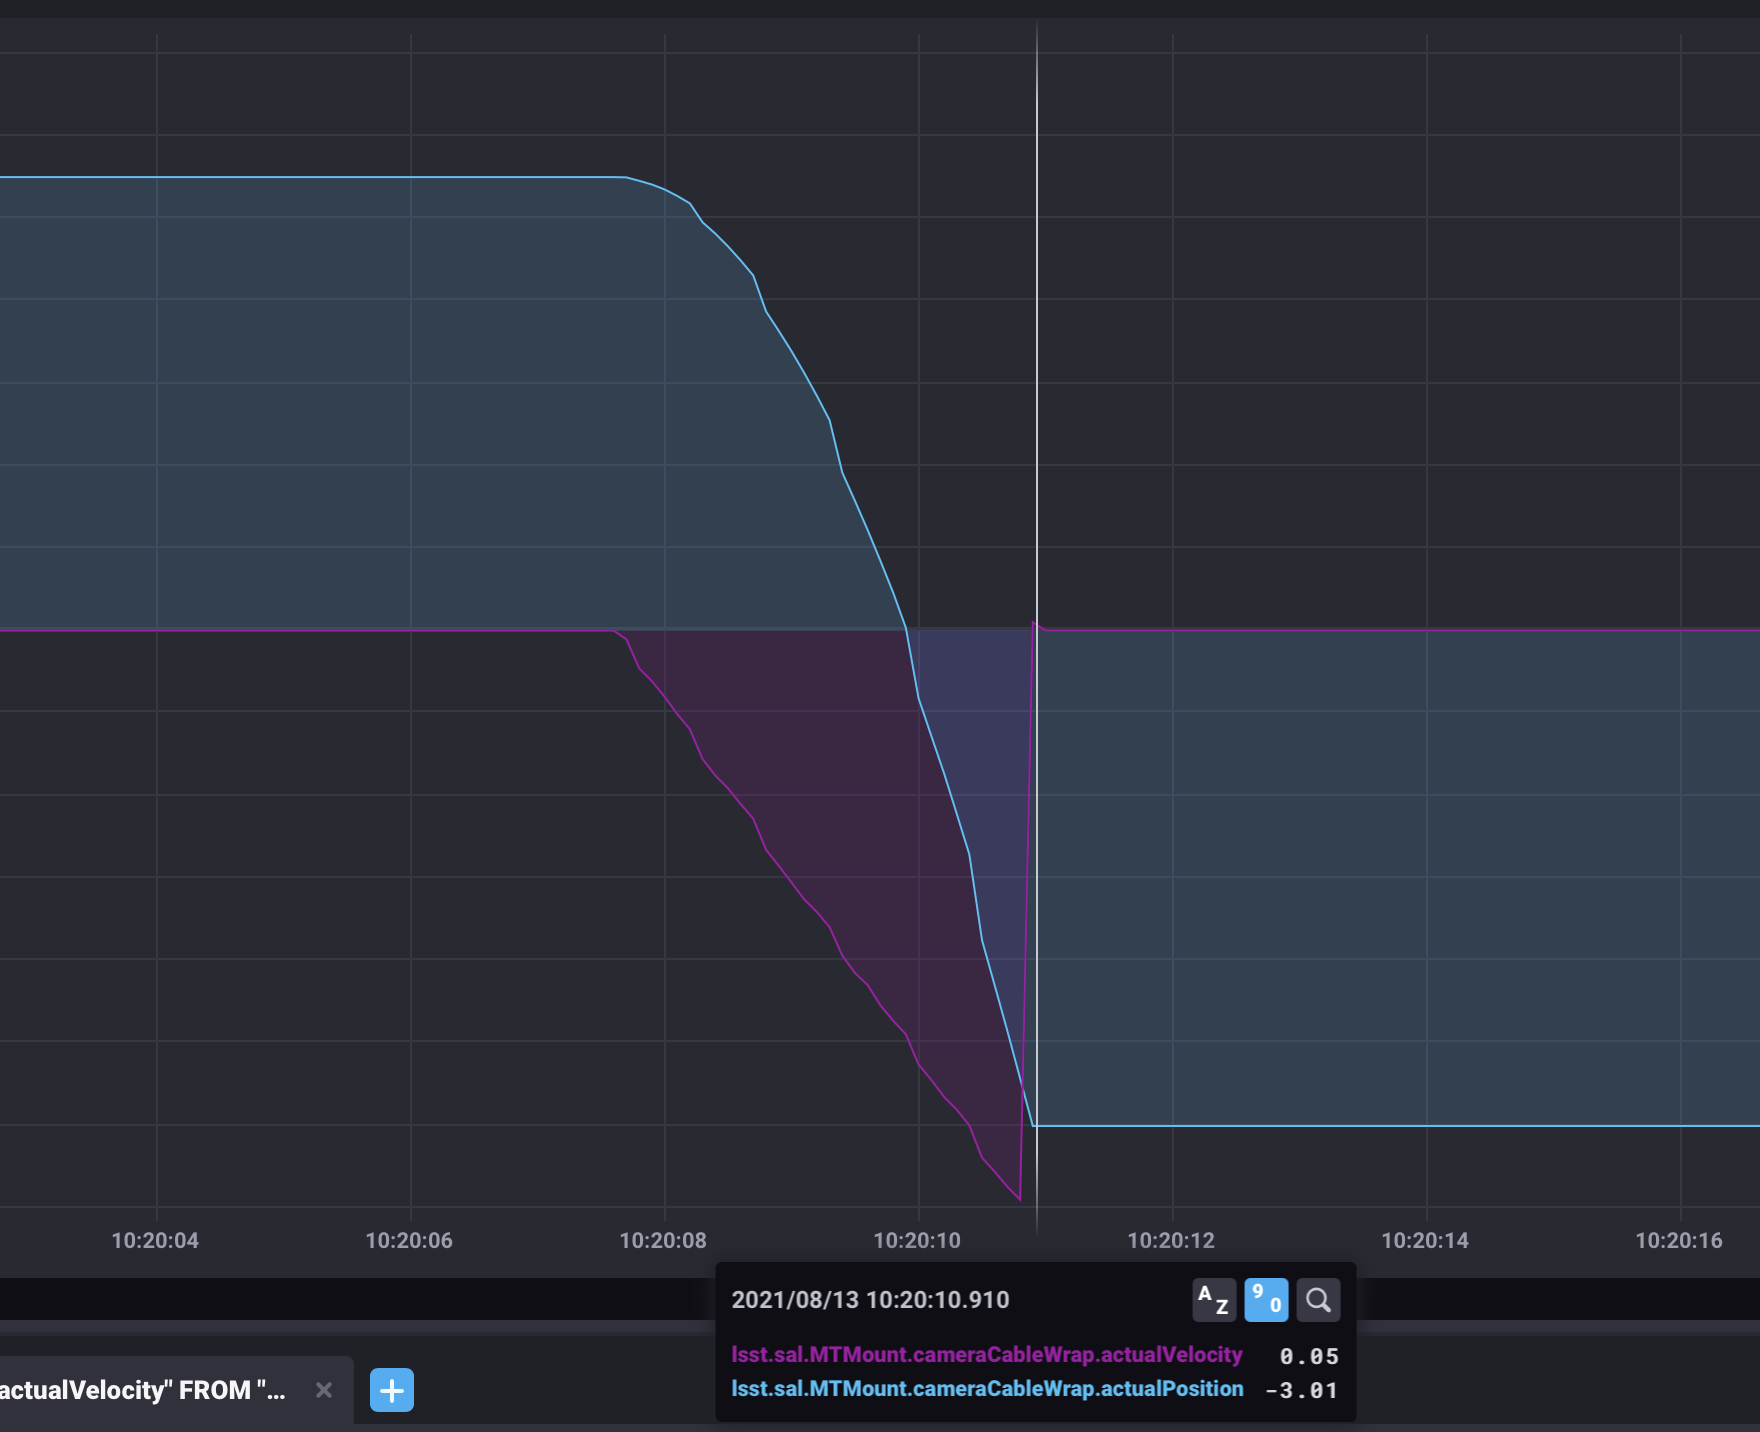
\includegraphics[width=\linewidth]{media/ccw_neg_4.png}
  \caption{CCW\_NEG\_RUN\_4}
  \label{fig:CCW_NEG_RUN_4}
\end{figure}

\begin{figure}
  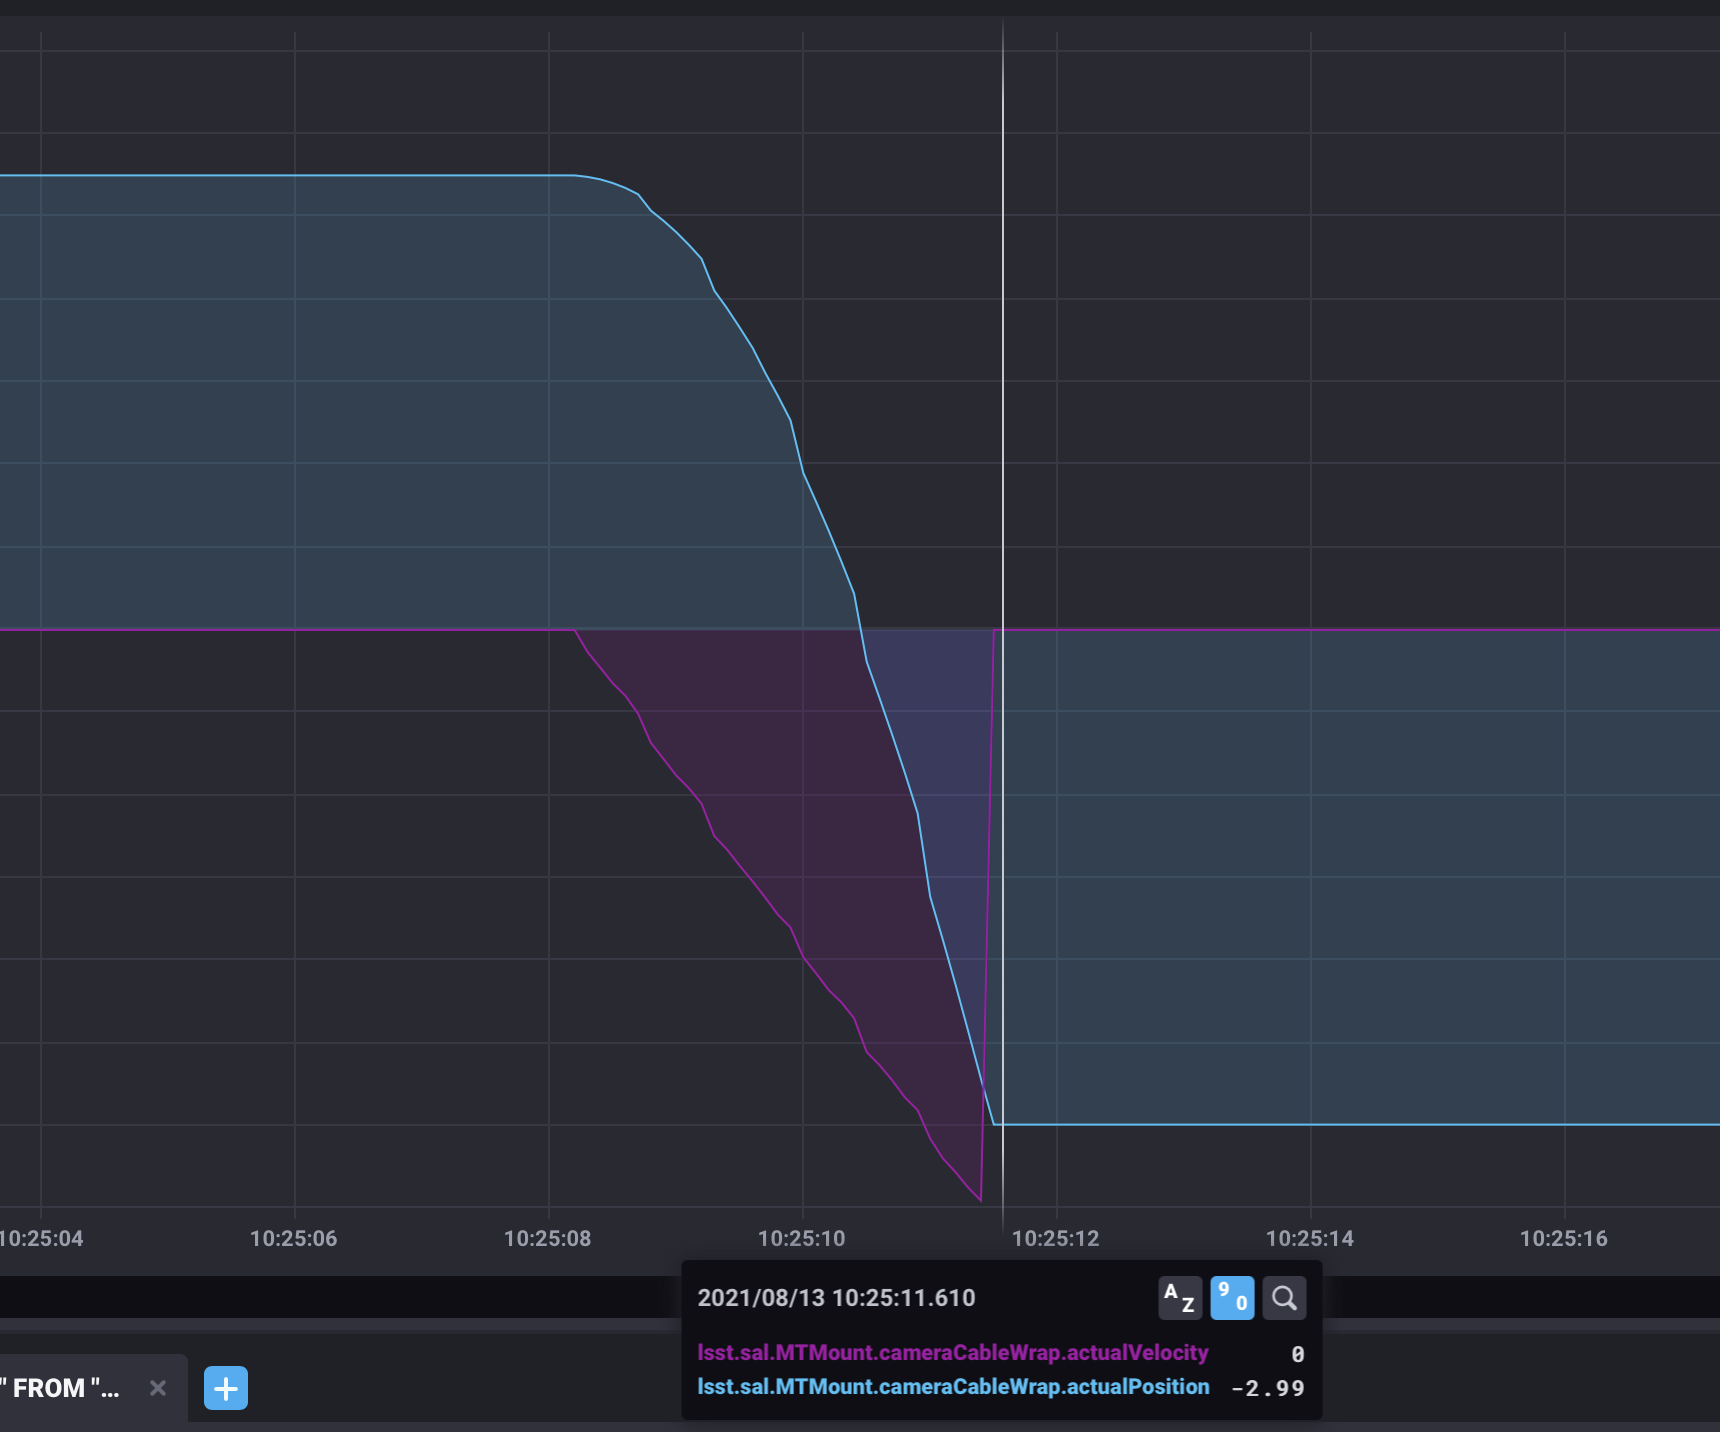
\includegraphics[width=\linewidth]{media/ccw_neg_5.png}
  \caption{CCW\_NEG\_RUN\_5}
  \label{fig:CCW_NEG_RUN_5}
\end{figure}
\newpage
\subsection{Rotator Positive Limit Switch EFD Data}
\begin{figure}
  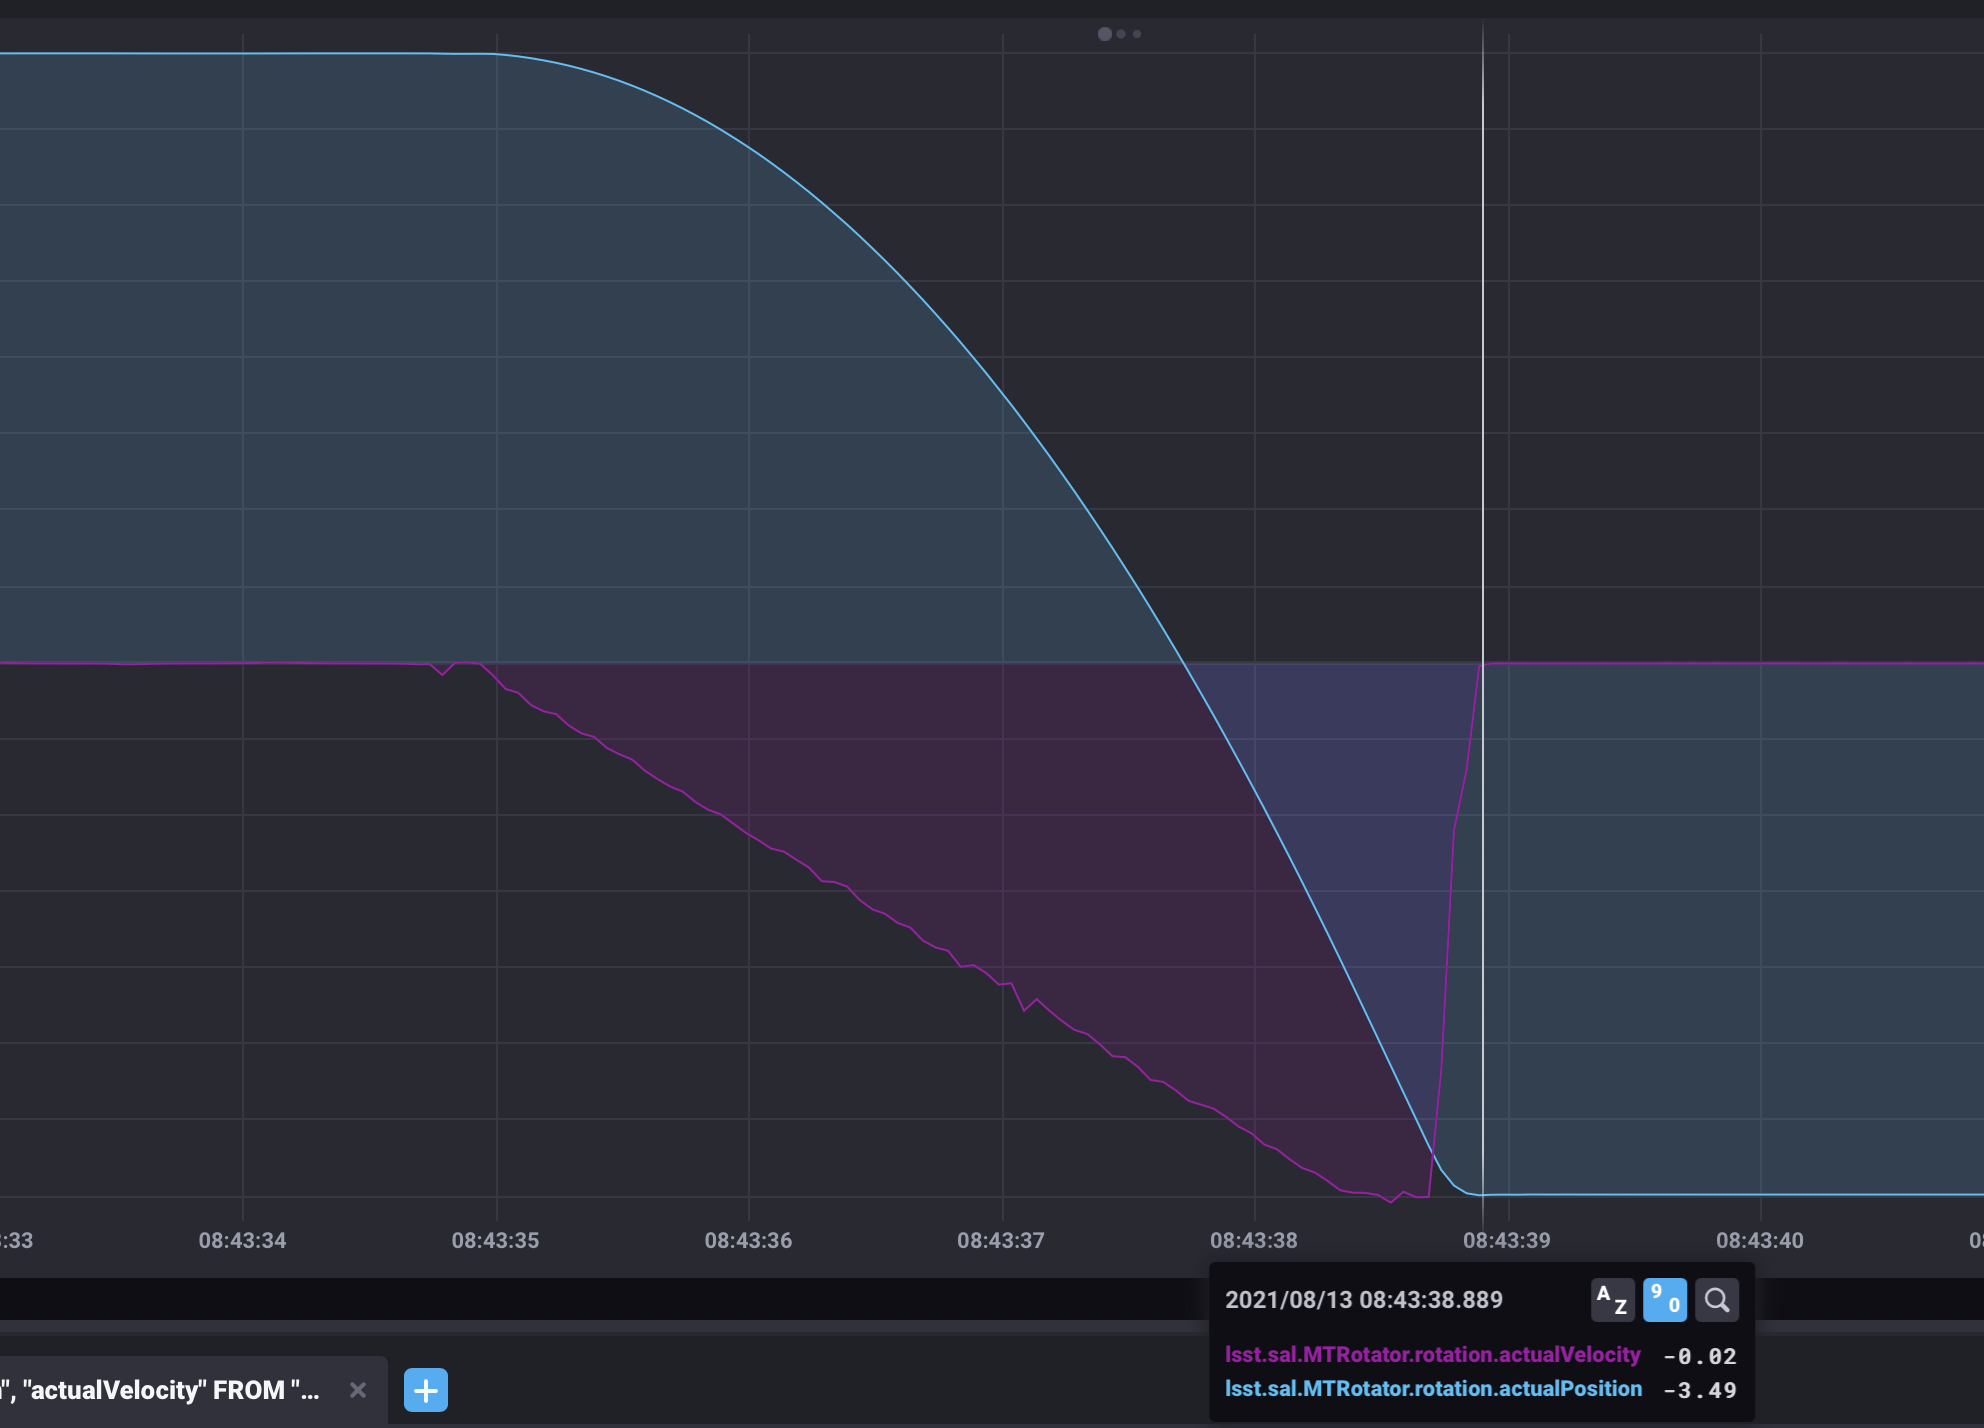
\includegraphics[width=\linewidth]{media/rotator_pos_1.png}
  \caption{Rotator\_POS\_RUN\_1}
  \label{fig:Rotator_POS_RUN_1}
\end{figure}

\begin{figure}
  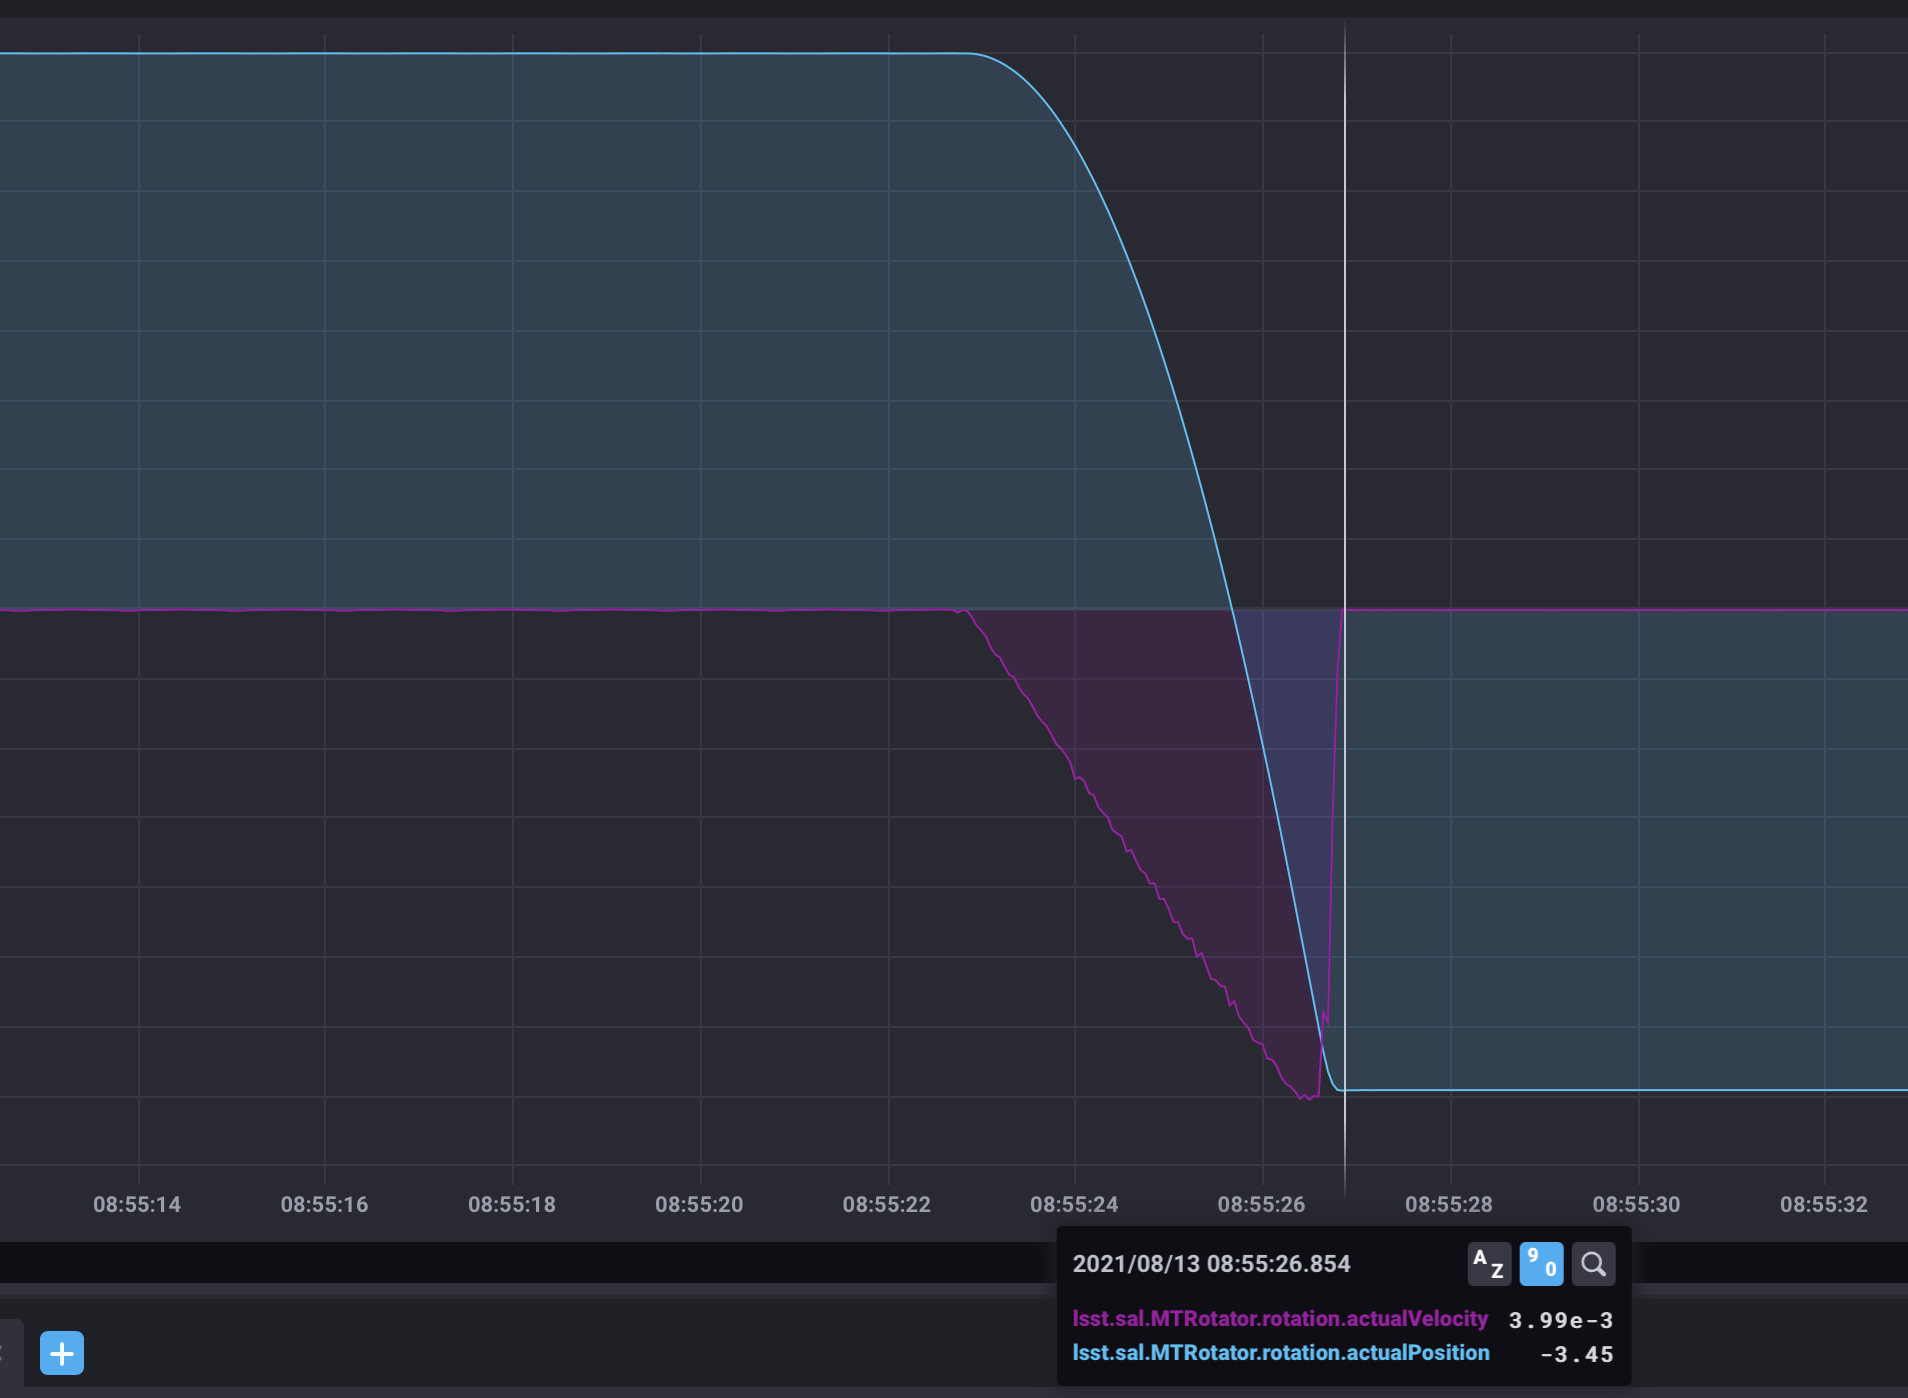
\includegraphics[width=\linewidth]{media/rotator_pos_2.png}
  \caption{Rotator\_POS\_RUN\_2}
  \label{fig:Rotator_POS_RUN_2}
\end{figure}

\begin{figure}
  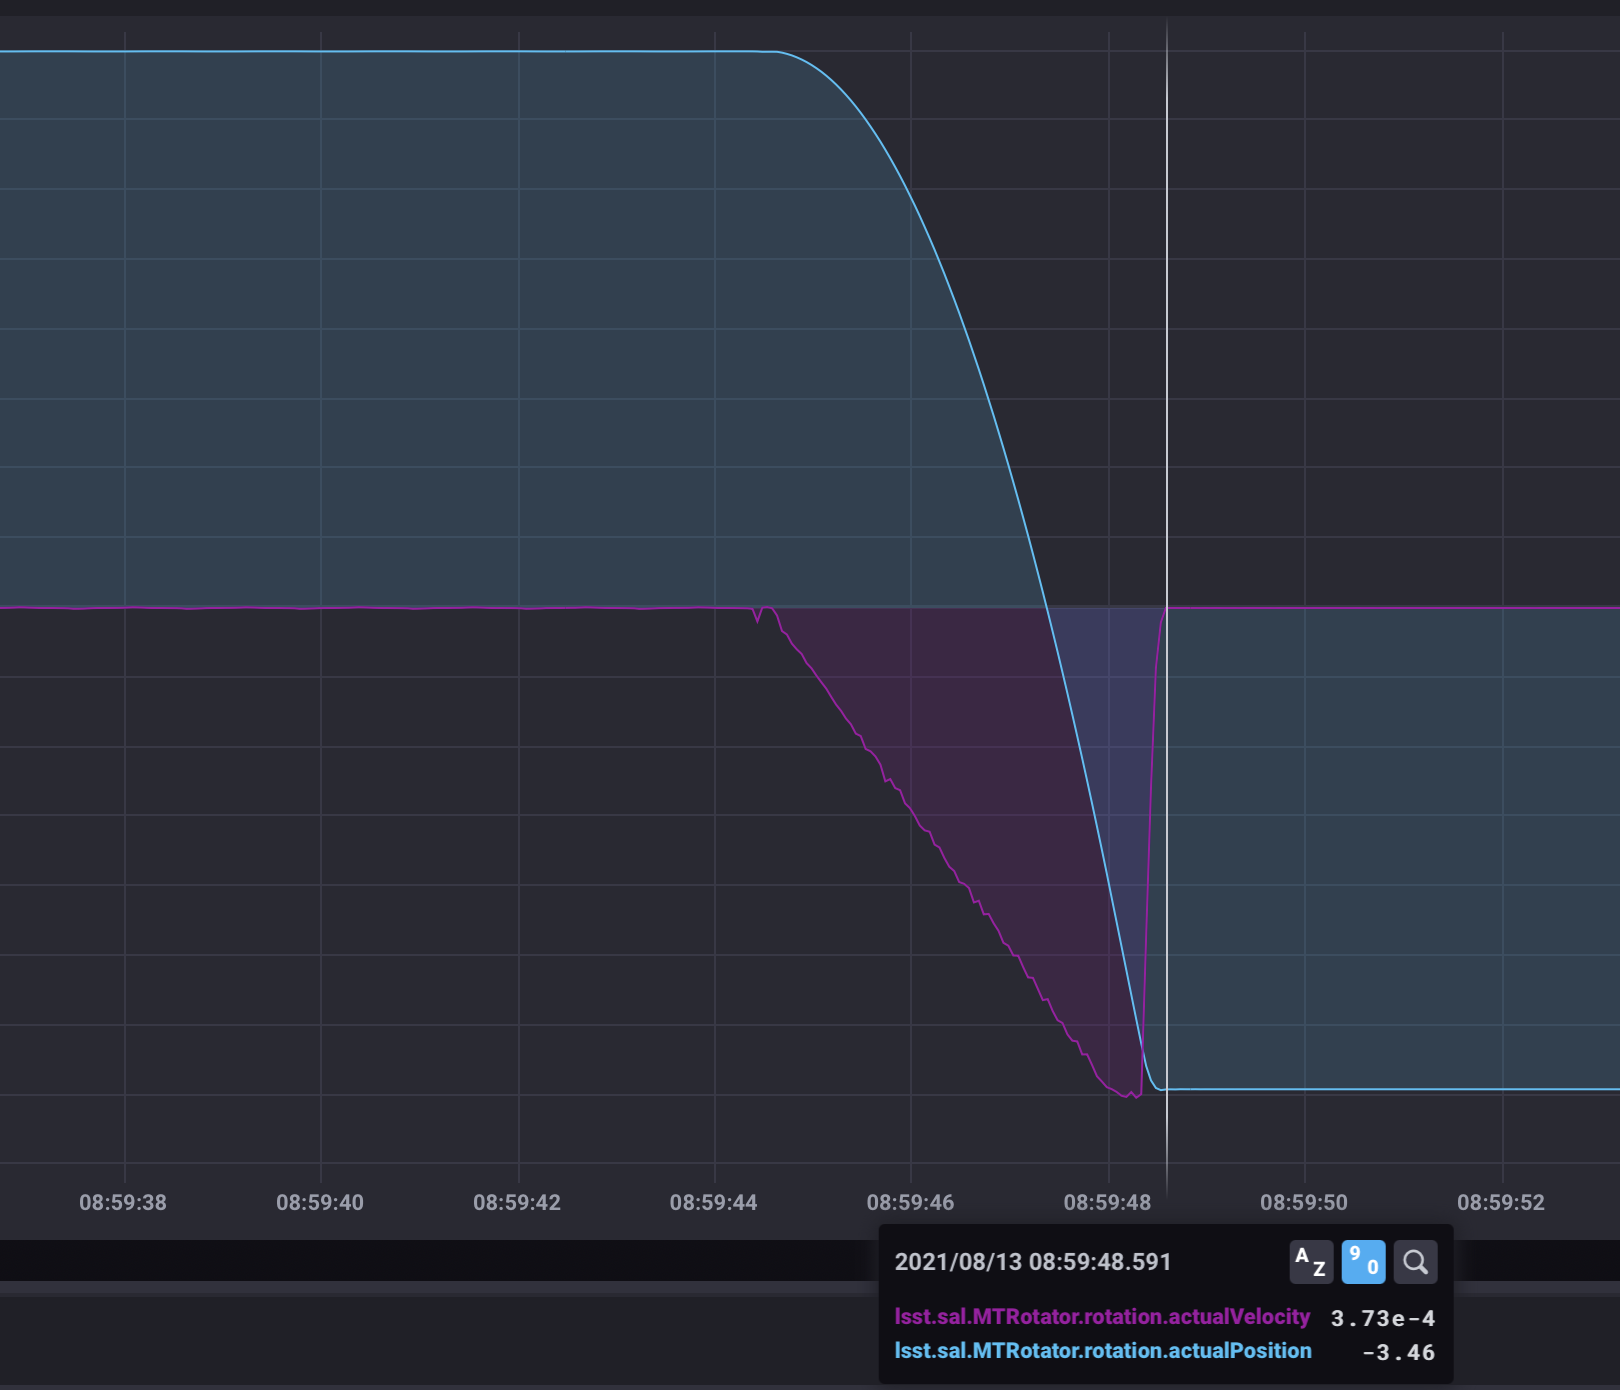
\includegraphics[width=\linewidth]{media/rotator_pos_3.png}
  \caption{Rotator\_POS\_RUN\_3}
  \label{fig:Rotator_POS_RUN_3}
\end{figure}

\begin{figure}
  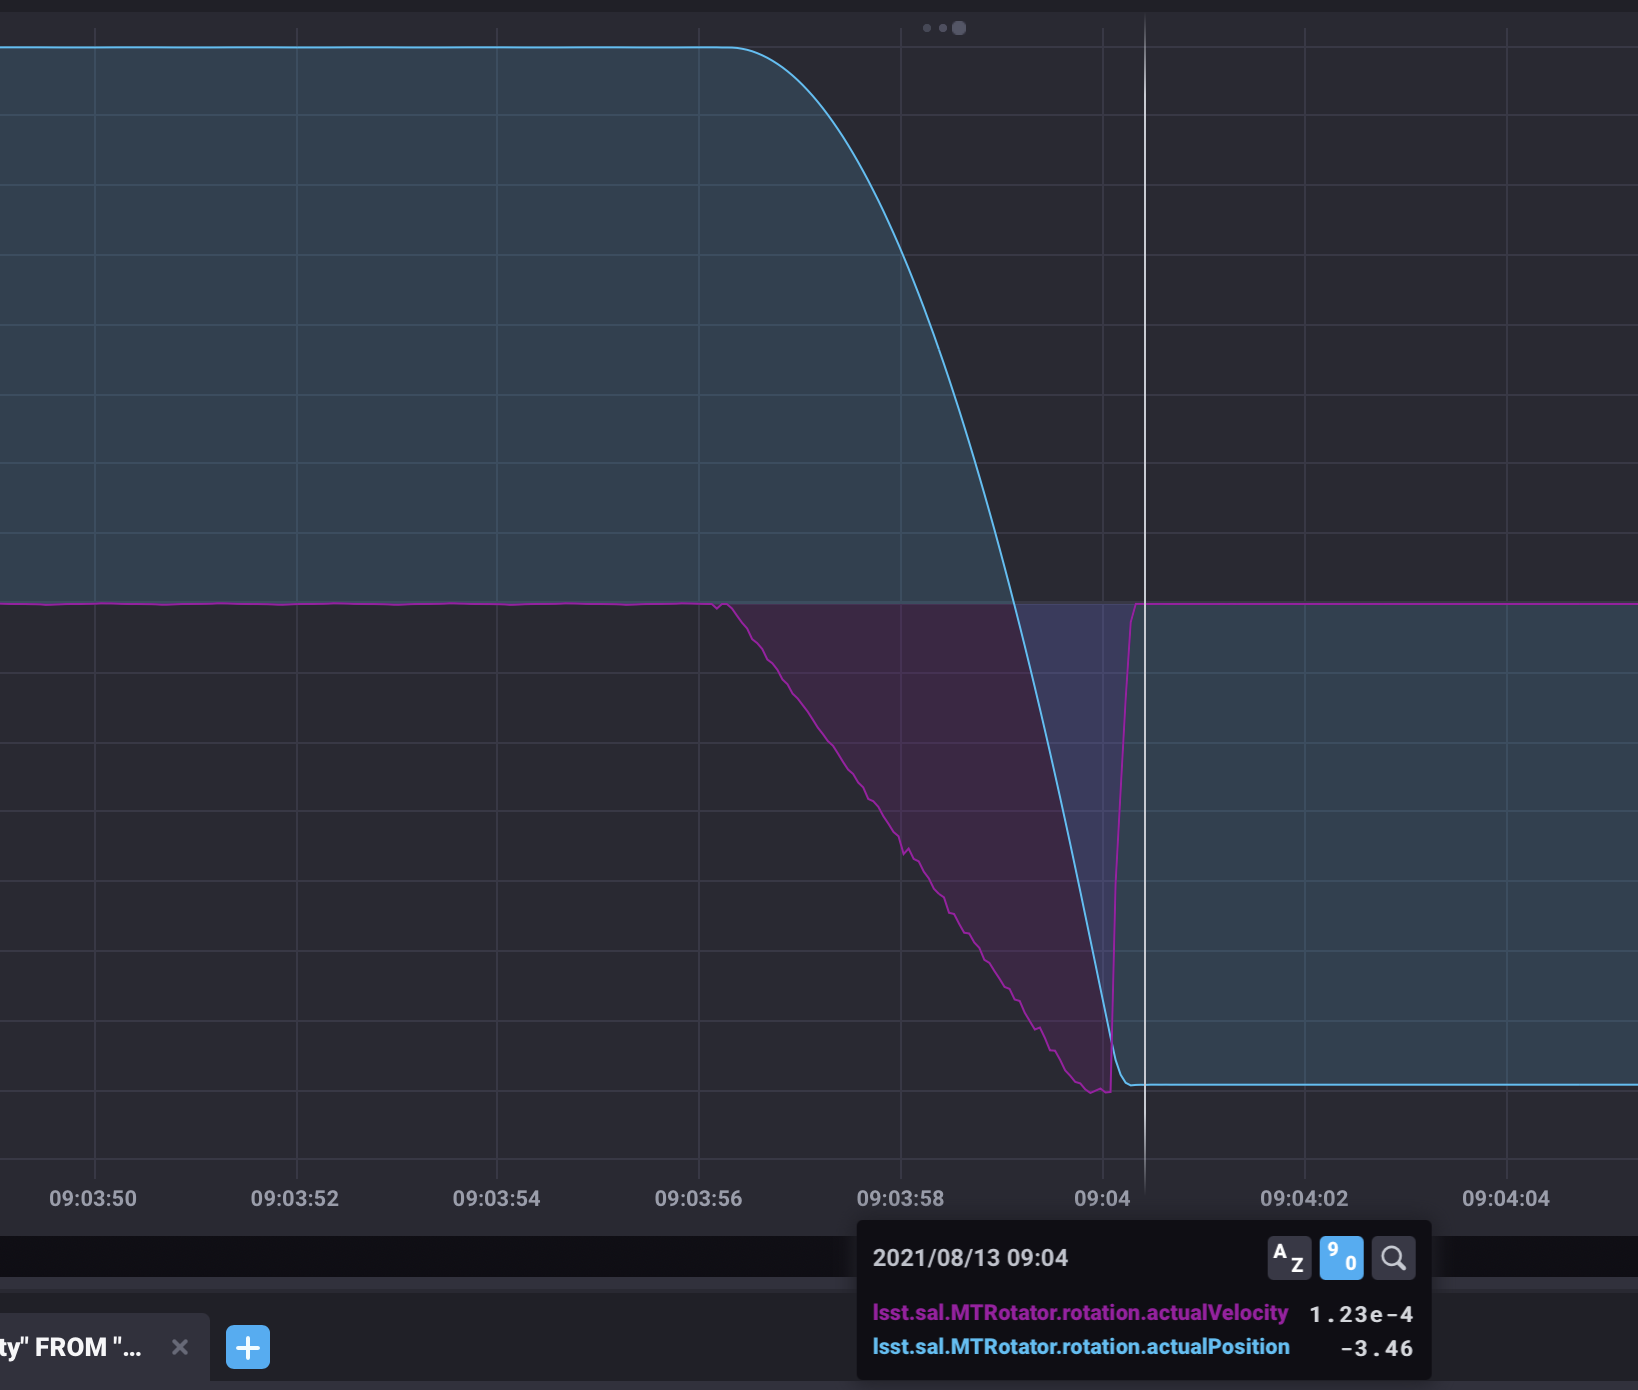
\includegraphics[width=\linewidth]{media/rotator_pos_4.png}
  \caption{Rotator\_POS\_RUN\_4}
  \label{fig:Rotator_POS_RUN_4}
\end{figure}

\begin{figure}
  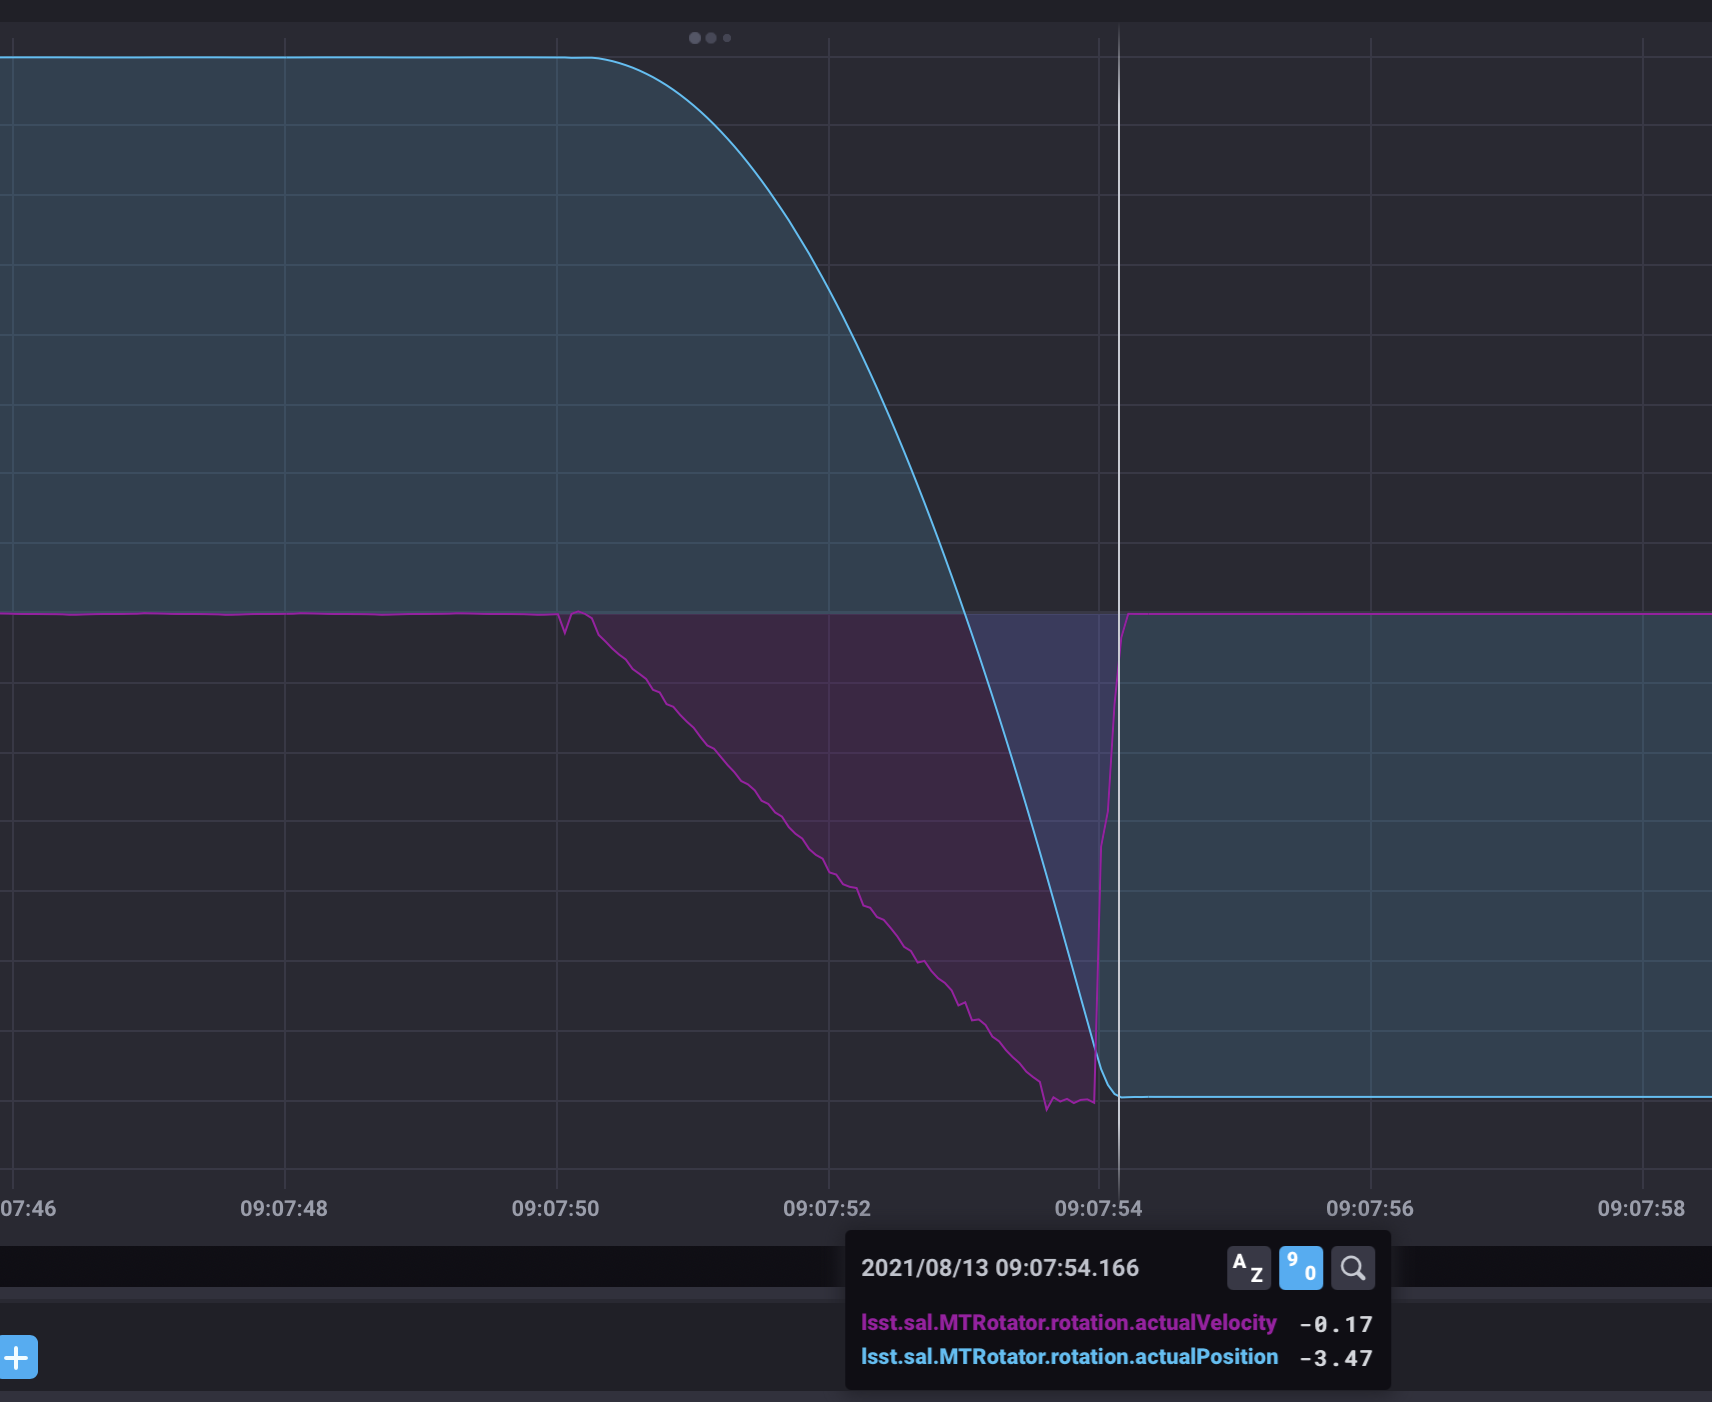
\includegraphics[width=\linewidth]{media/rotator_pos_5.png}
  \caption{Rotator\_POS\_RUN\_5}
  \label{fig:Rotator_POS_RUN_5}
\end{figure}
\newpage
\subsection{Rotator Negative Limit Switch EFD Data}
\begin{figure}
  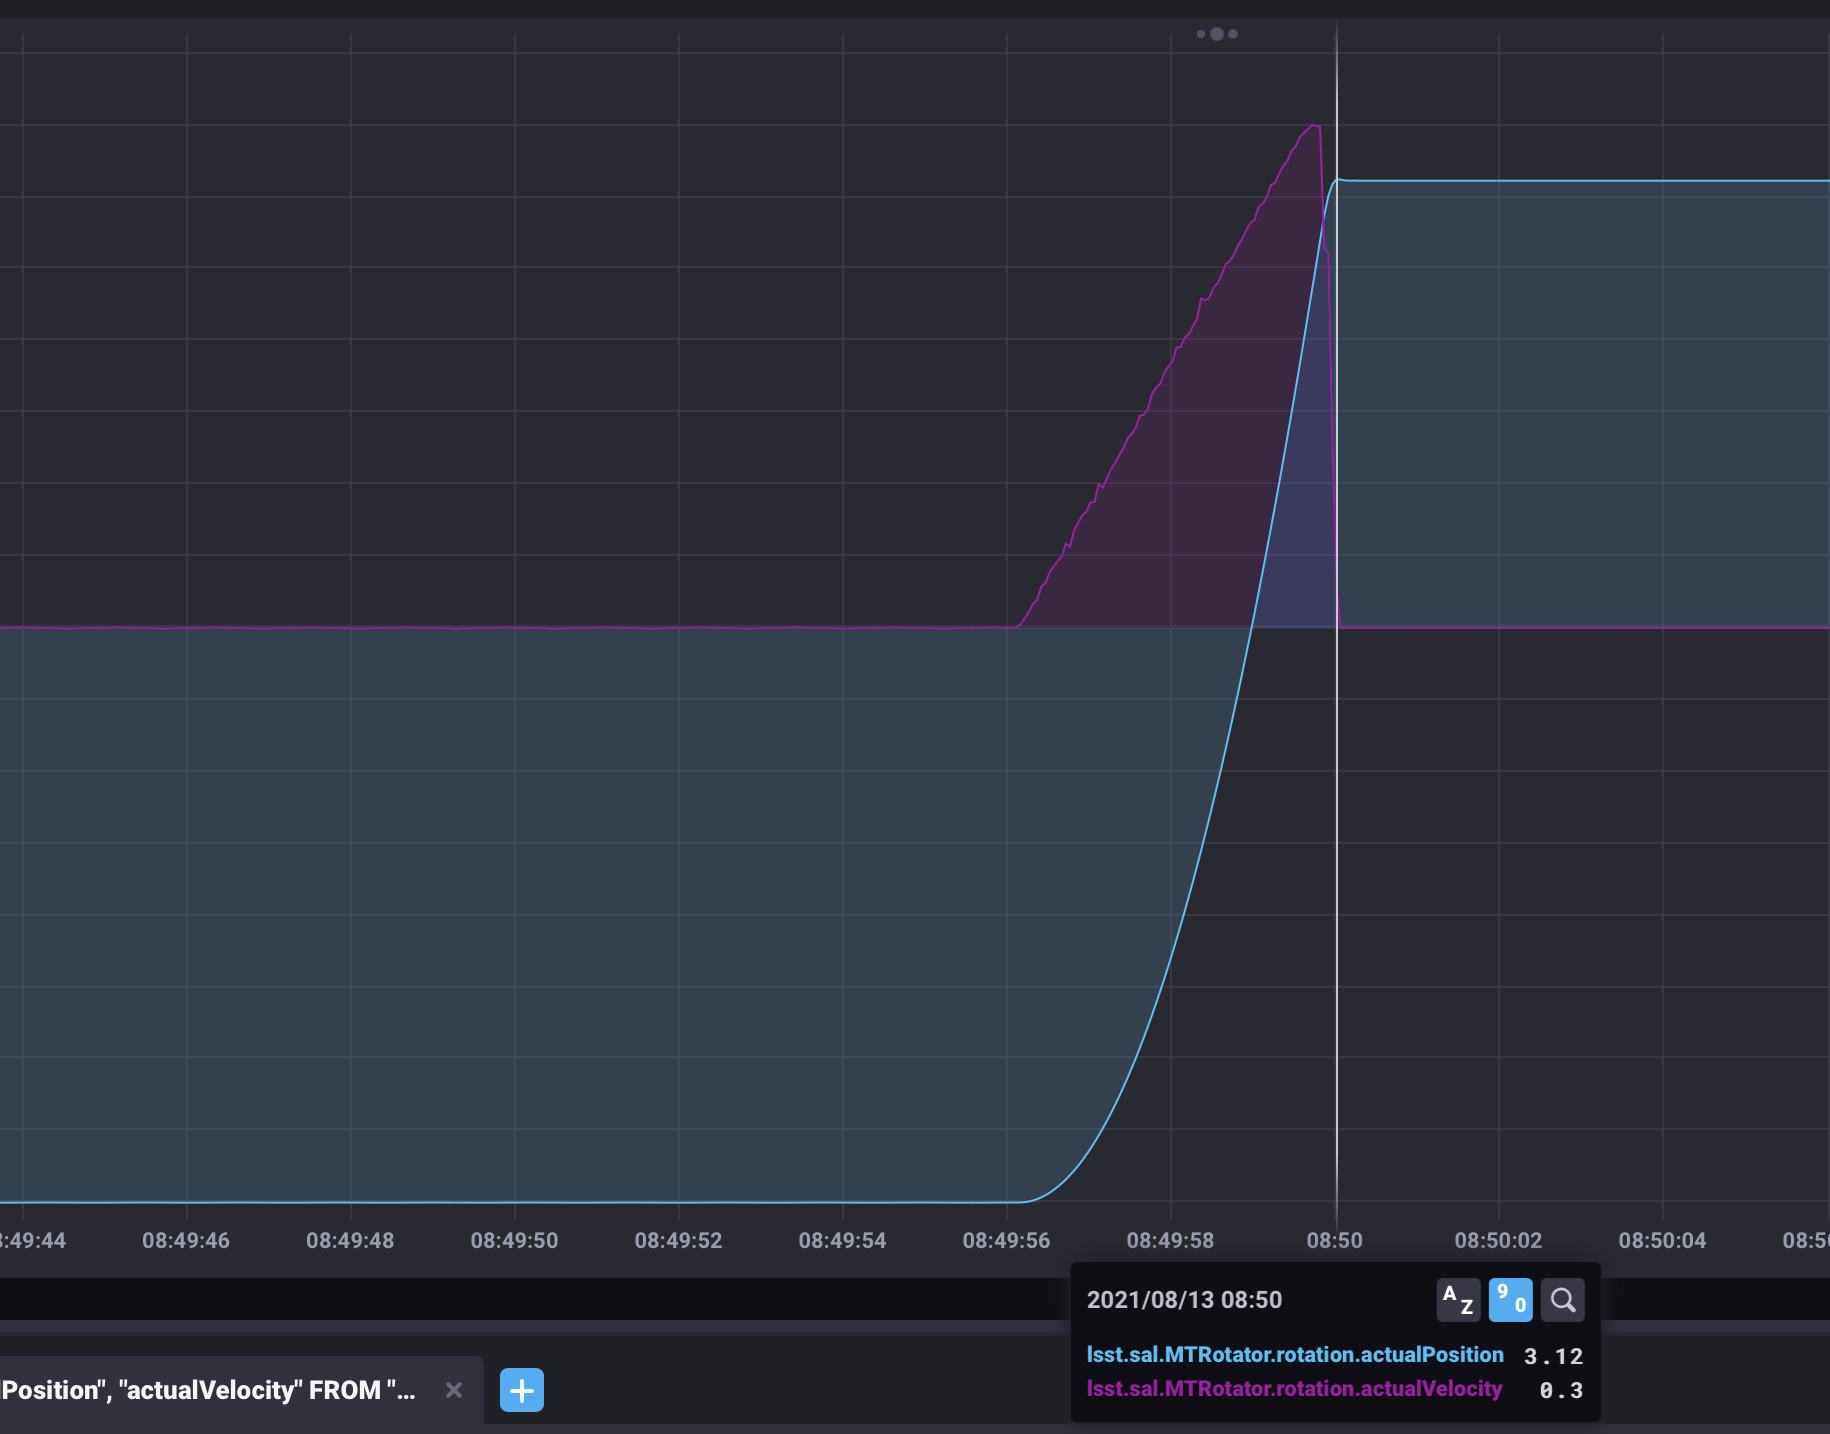
\includegraphics[width=\linewidth]{media/rotator_neg_1.png}
  \caption{Rotator\_NEG\_RUN\_1}
  \label{fig:Rotator_NEG_RUN_1}
\end{figure}

\begin{figure}
  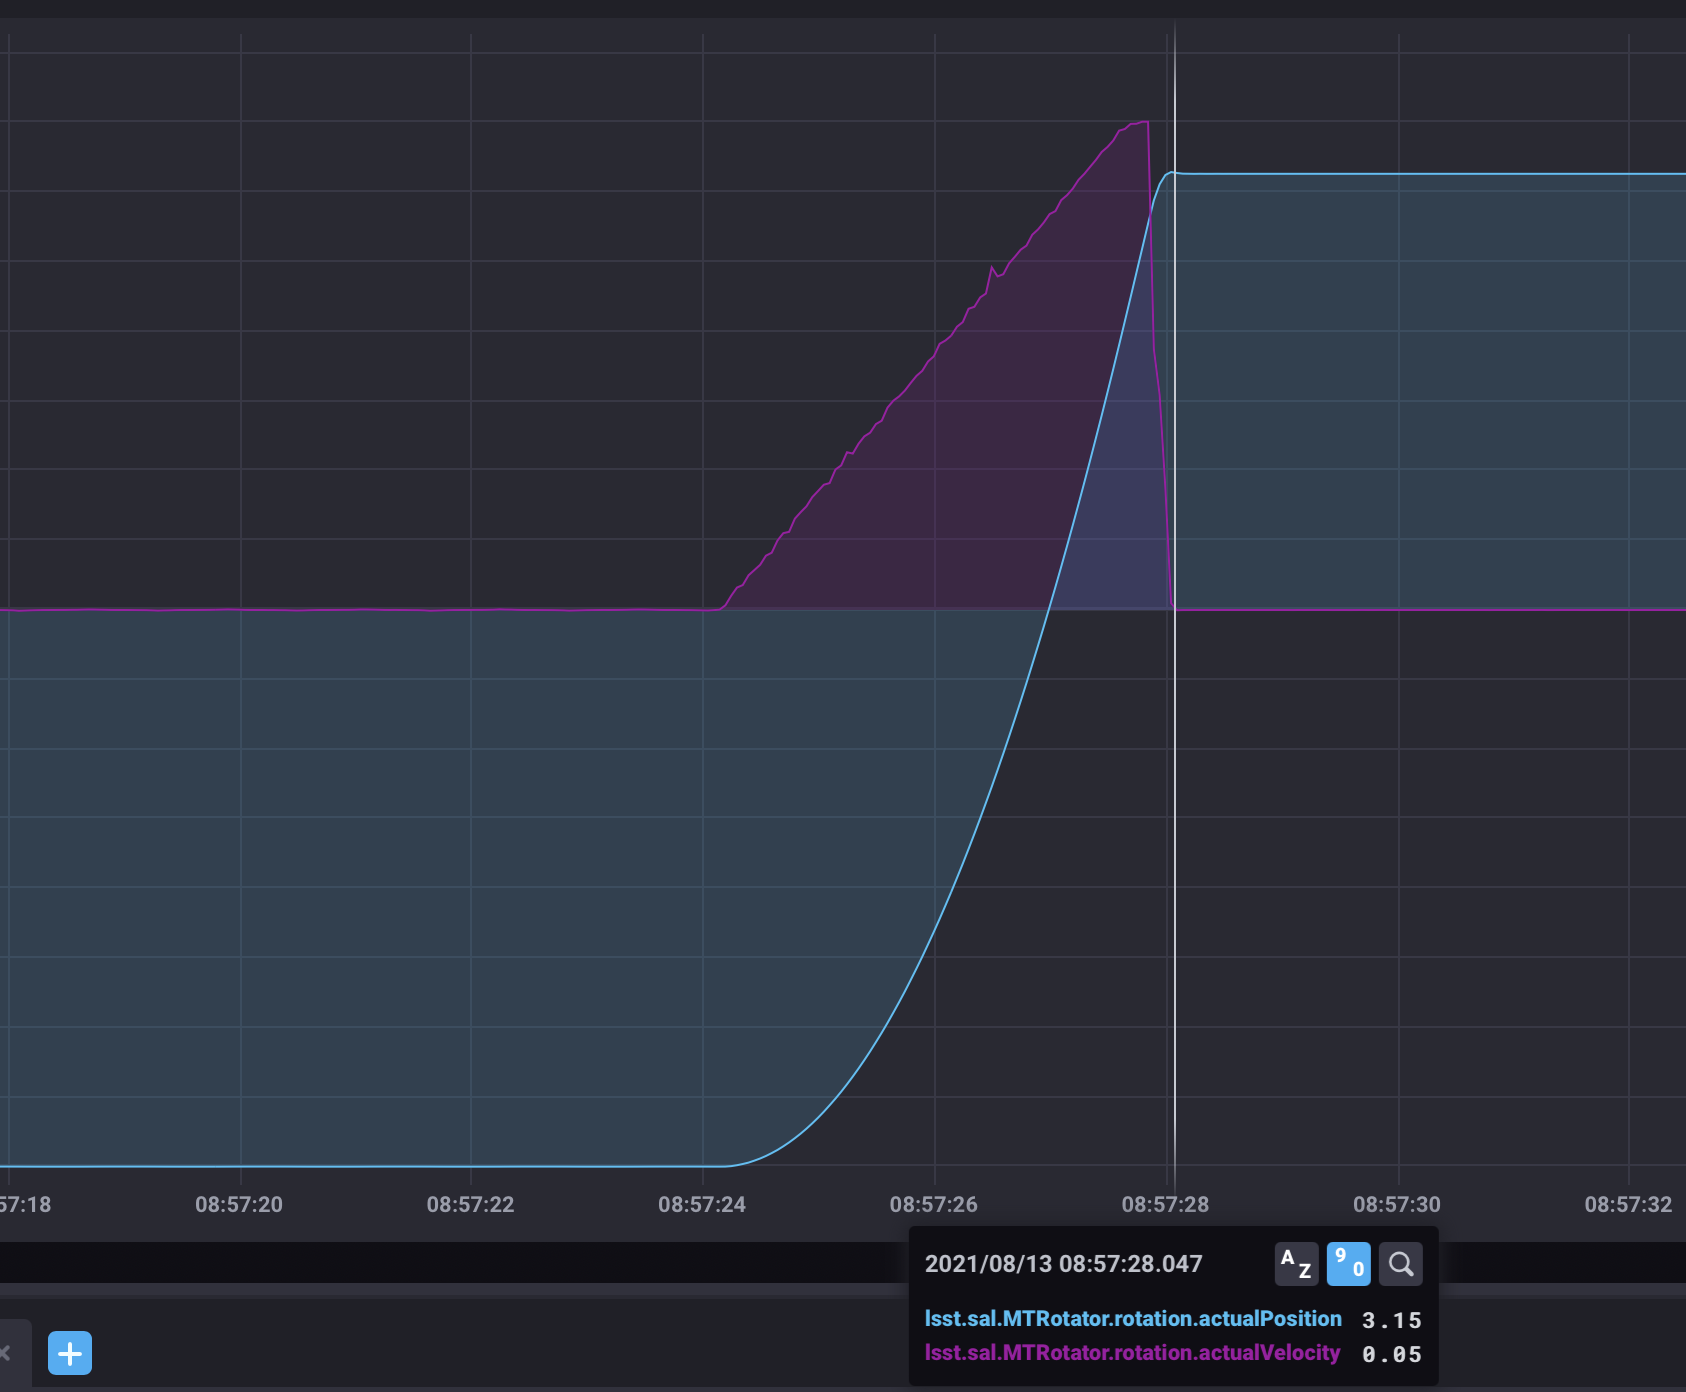
\includegraphics[width=\linewidth]{media/rotator_neg_2.png}
  \caption{Rotator\_NEG\_RUN\_2}
  \label{fig:Rotator_NEG_RUN_2}
\end{figure}

\begin{figure}
  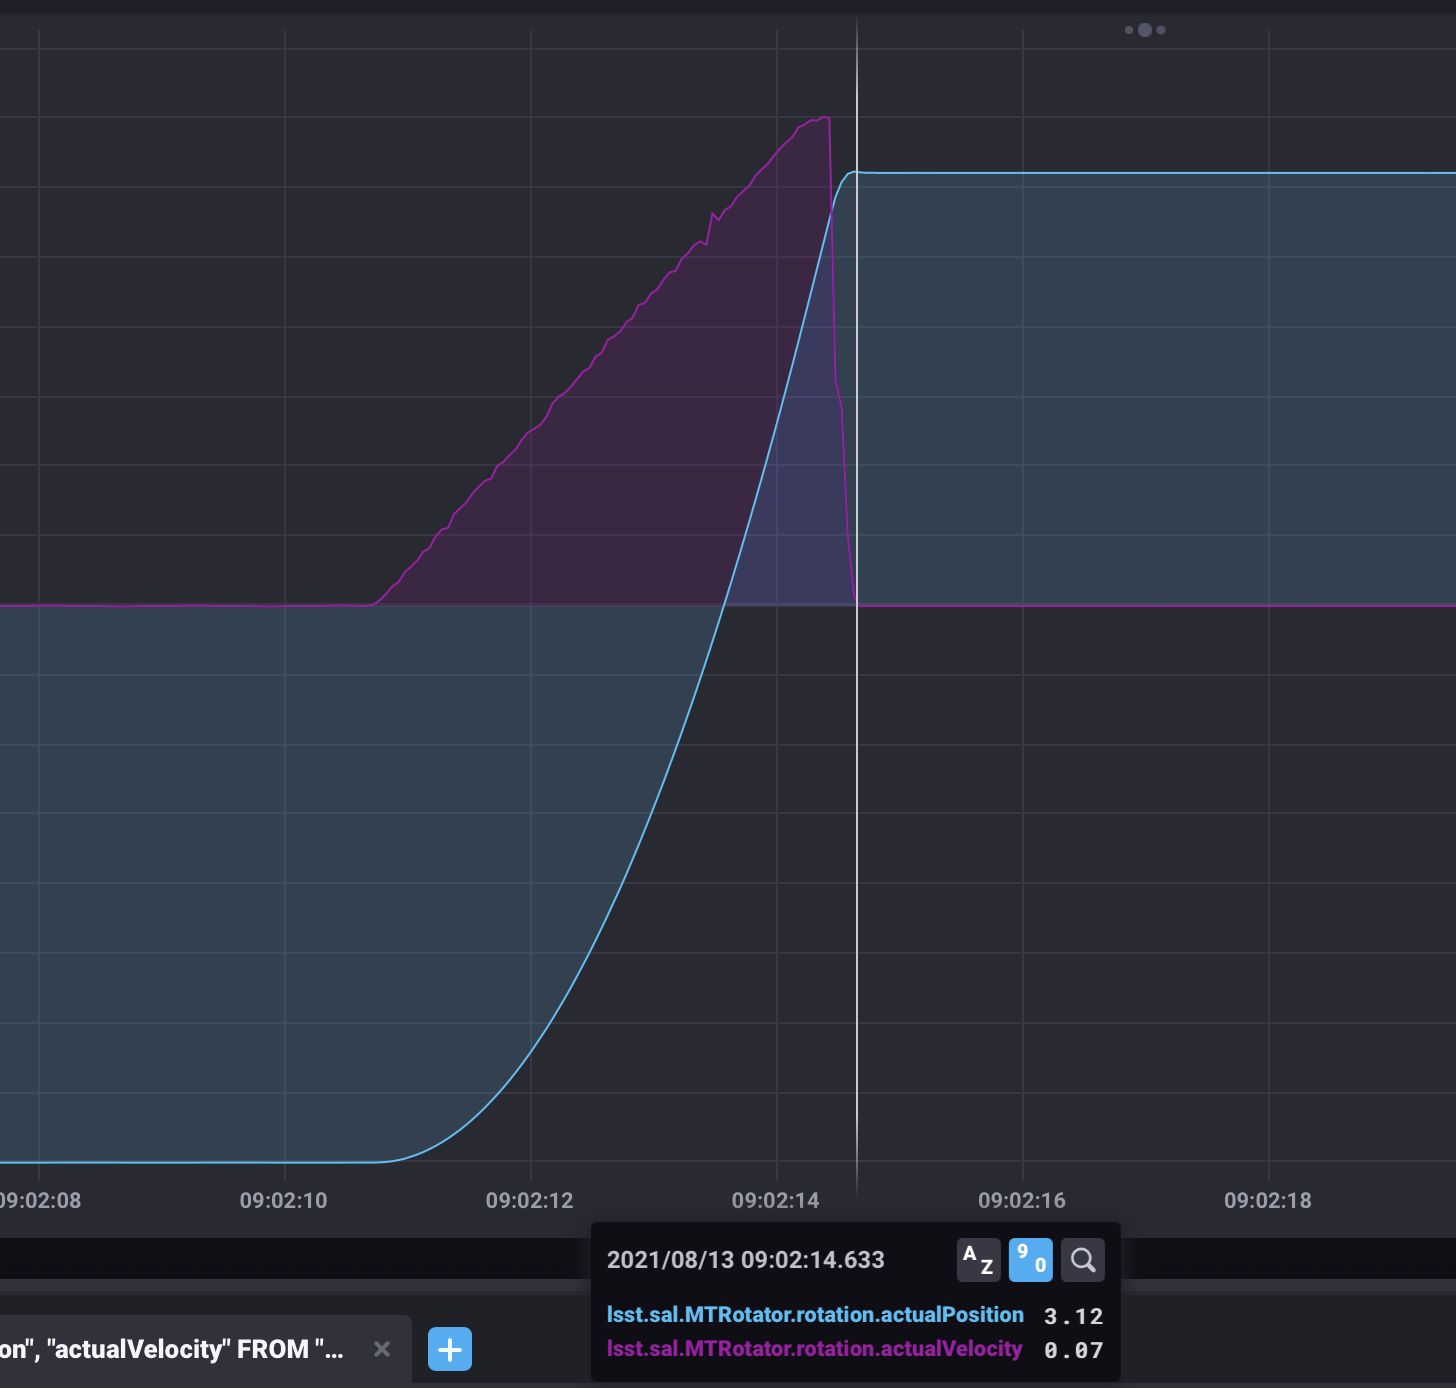
\includegraphics[width=\linewidth]{media/rotator_neg_3.png}
  \caption{Rotator\_NEG\_RUN\_3}
  \label{fig:Rotator_NEG_RUN_3}
\end{figure}

\begin{figure}
  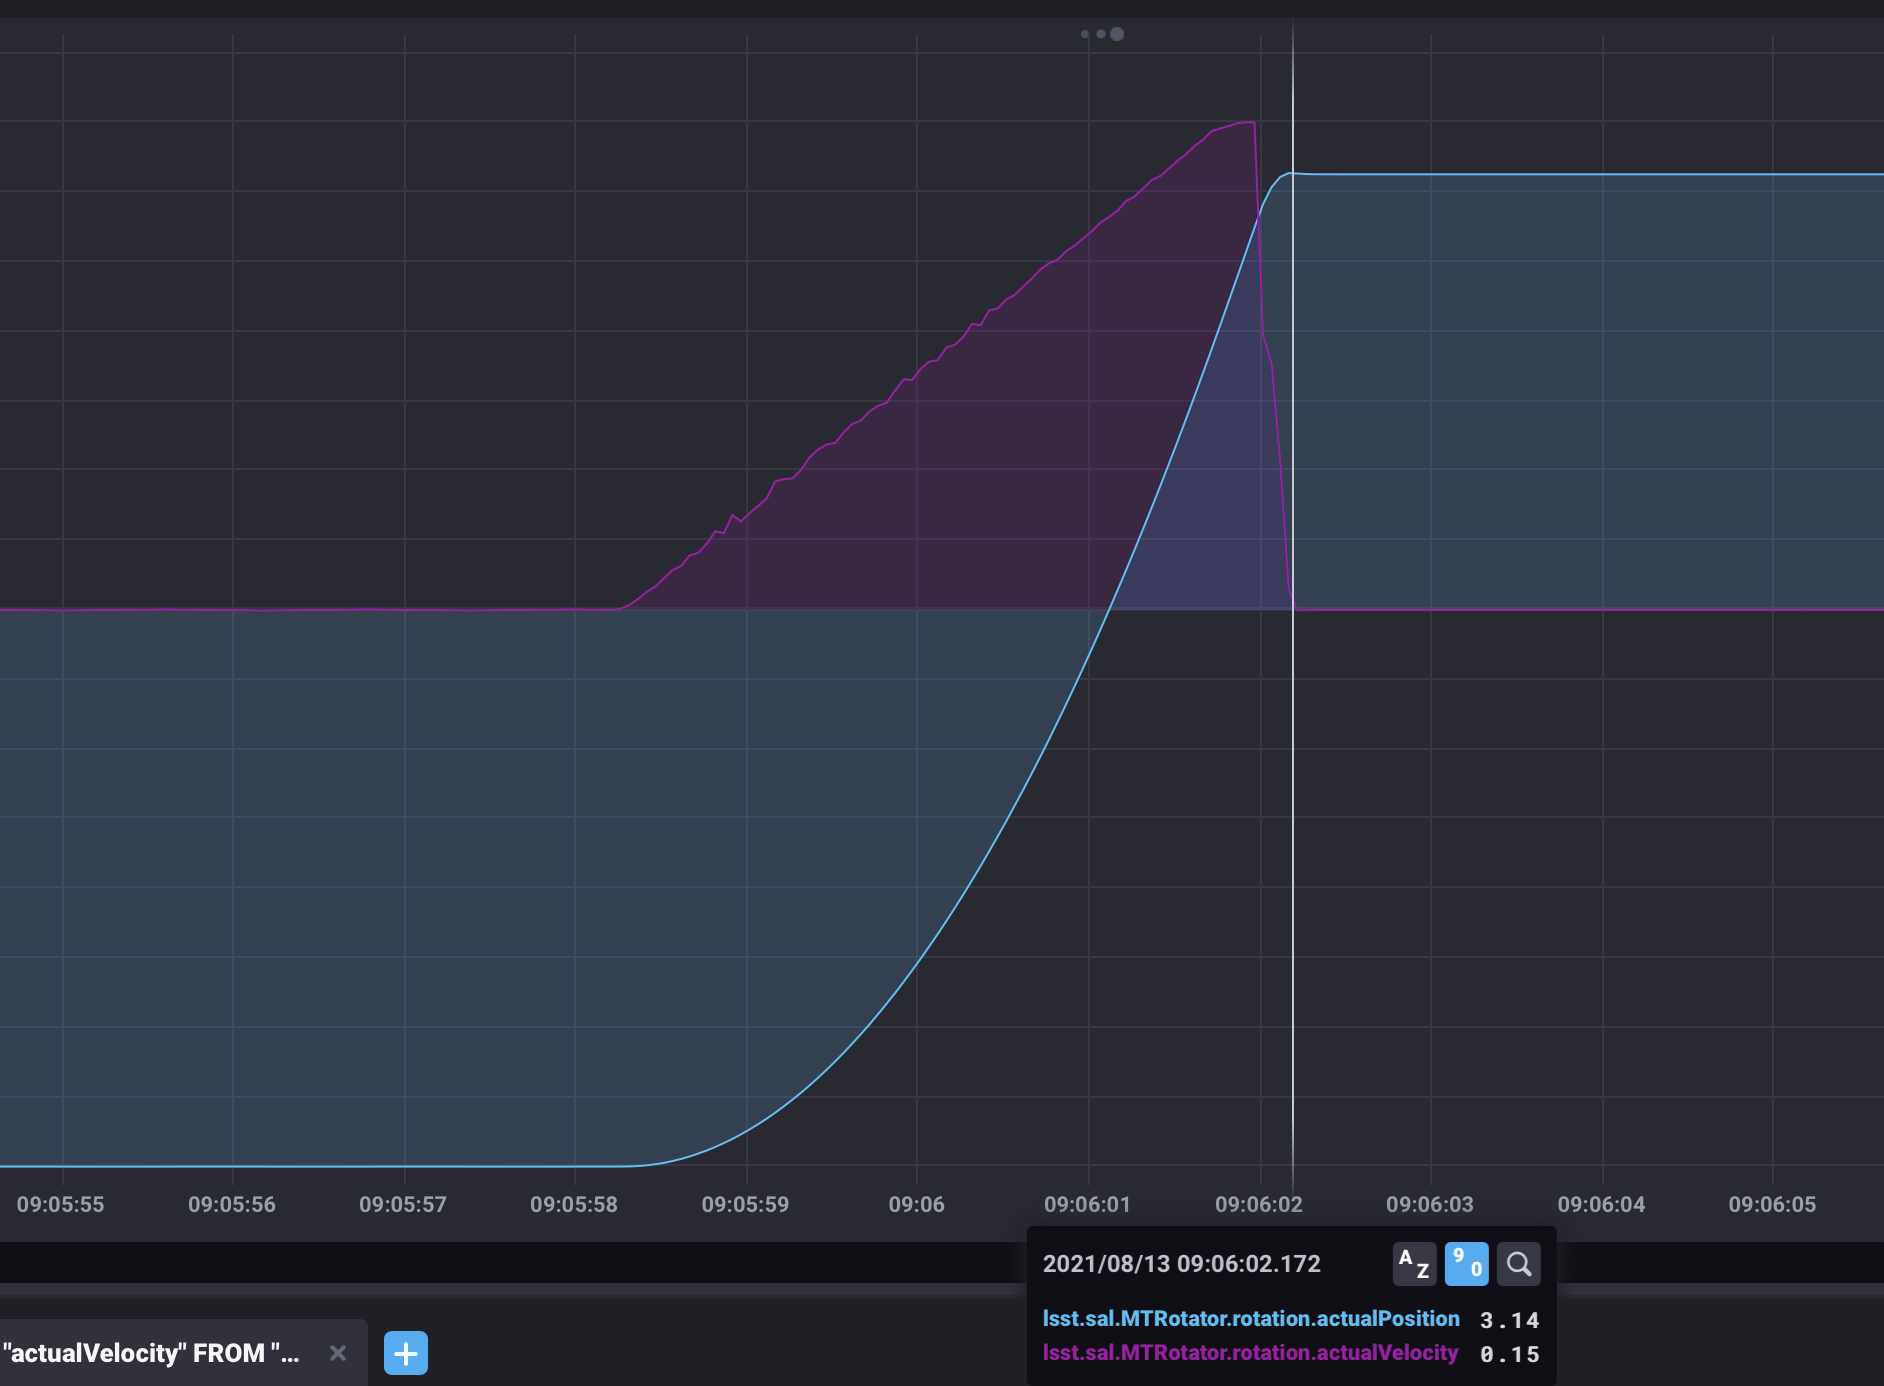
\includegraphics[width=\linewidth]{media/rotator_neg_4.png}
  \caption{Rotator\_NEG\_RUN\_4}
  \label{fig:Rotator_NEG_RUN_4}
\end{figure}

\begin{figure}
  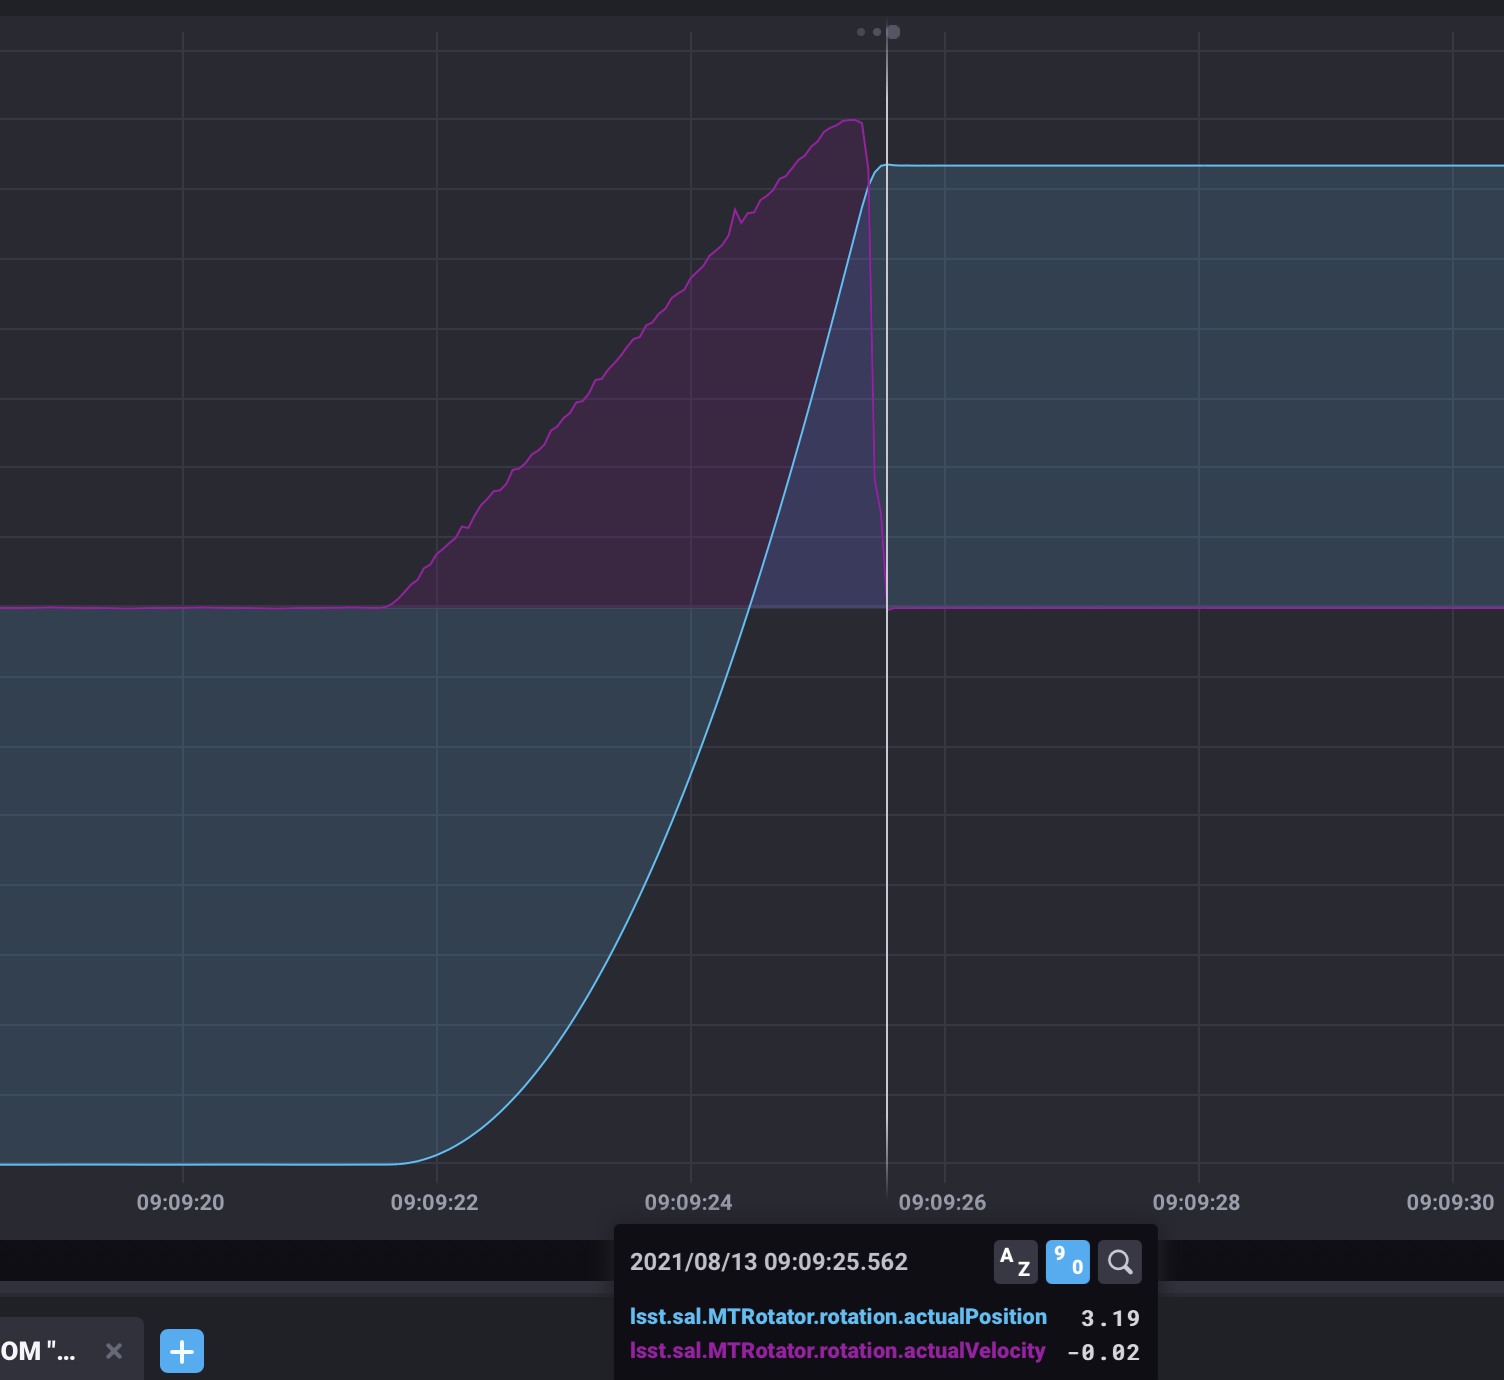
\includegraphics[width=\linewidth]{media/rotator_neg_5.png}
  \caption{Rotator\_NEG\_RUN\_5}
  \label{fig:Rotator_NEG_RUN_5}
\end{figure}
\newpage
\subsection{Normal Operating Conditions EFD Data}
\begin{figure}
  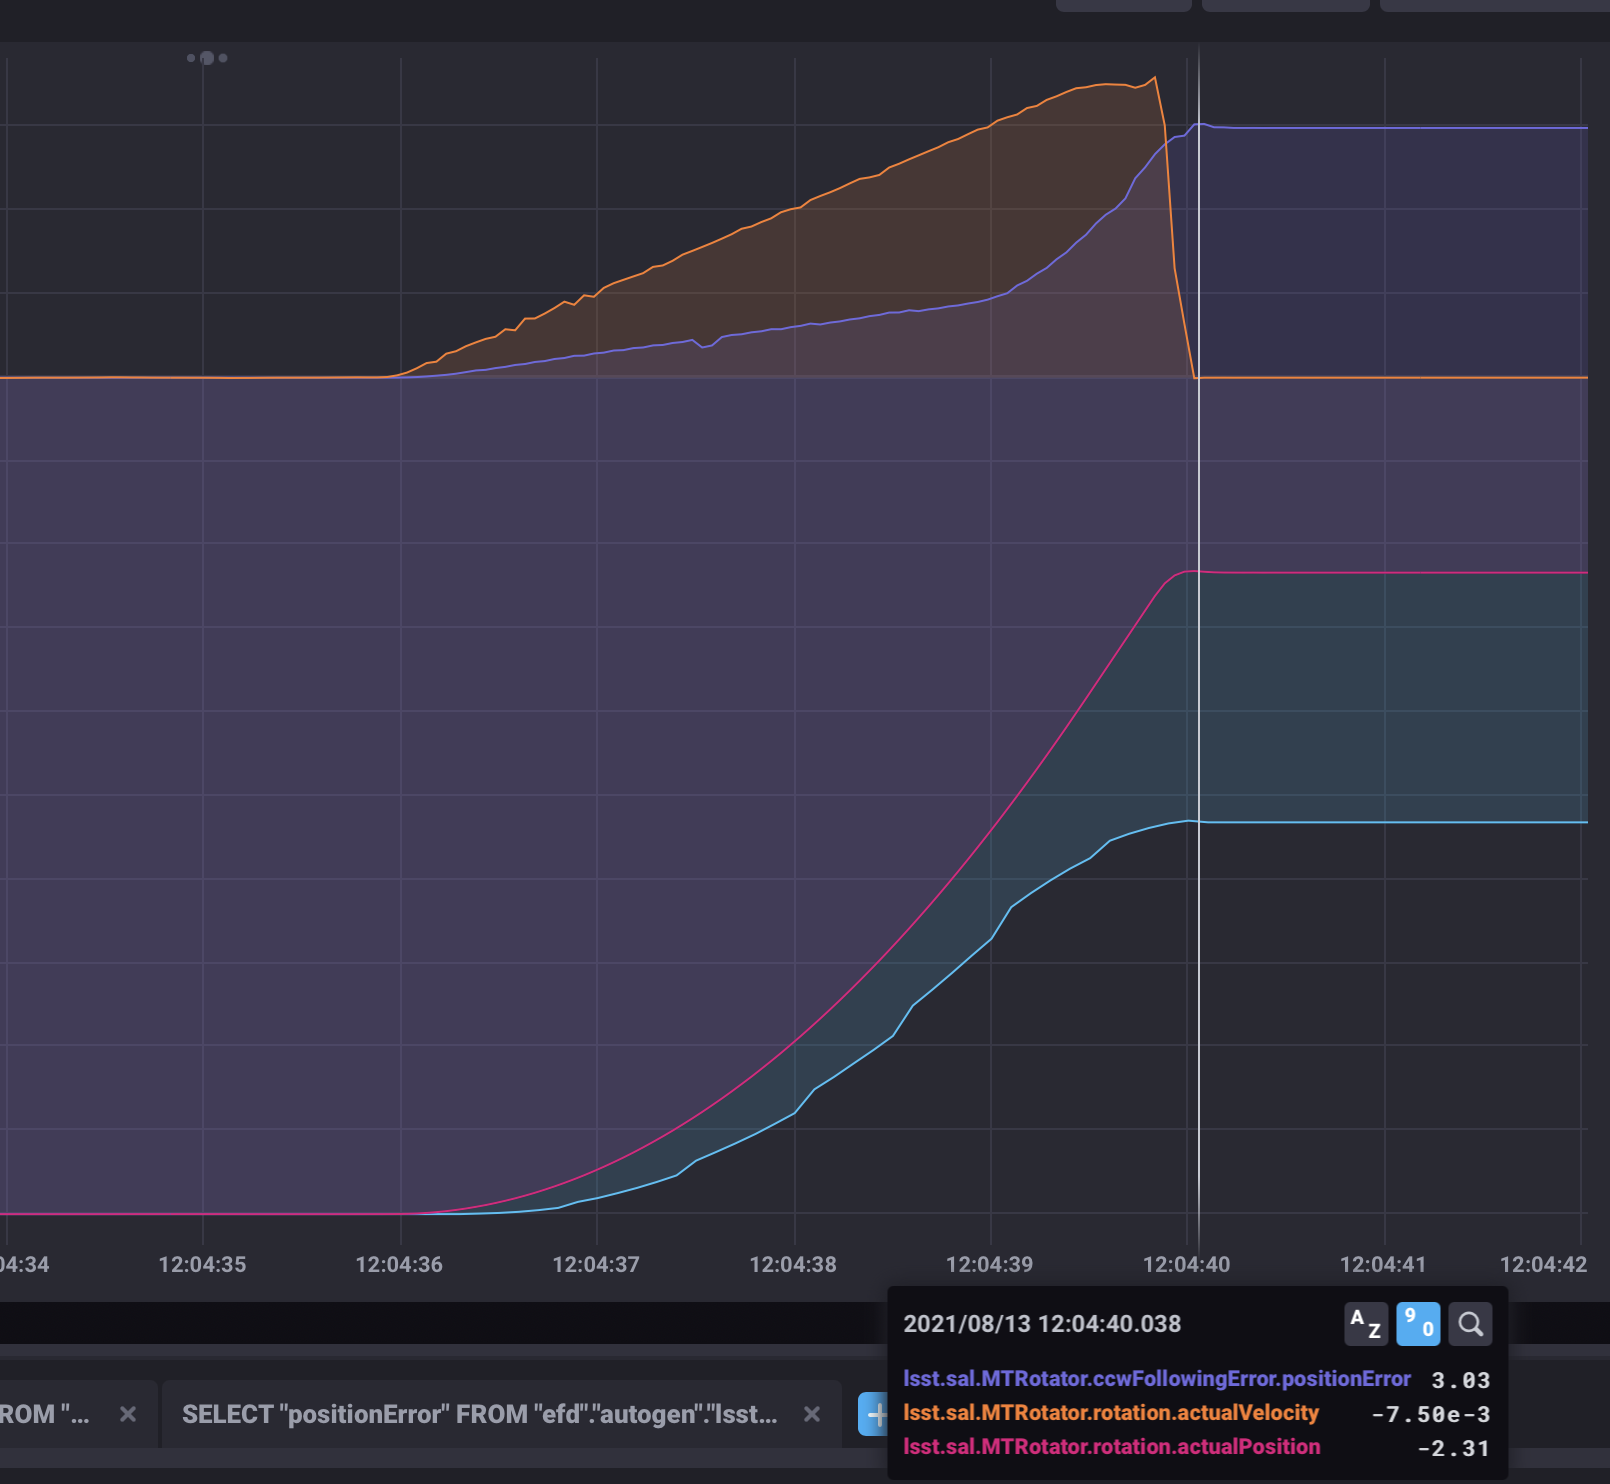
\includegraphics[width=\linewidth]{media/followingFault_1.png}
  \caption{Normal\_Conditions\_RUN\_1}
  \label{fig:Normal_Conditions_RUN_1}
\end{figure}

\begin{figure}
  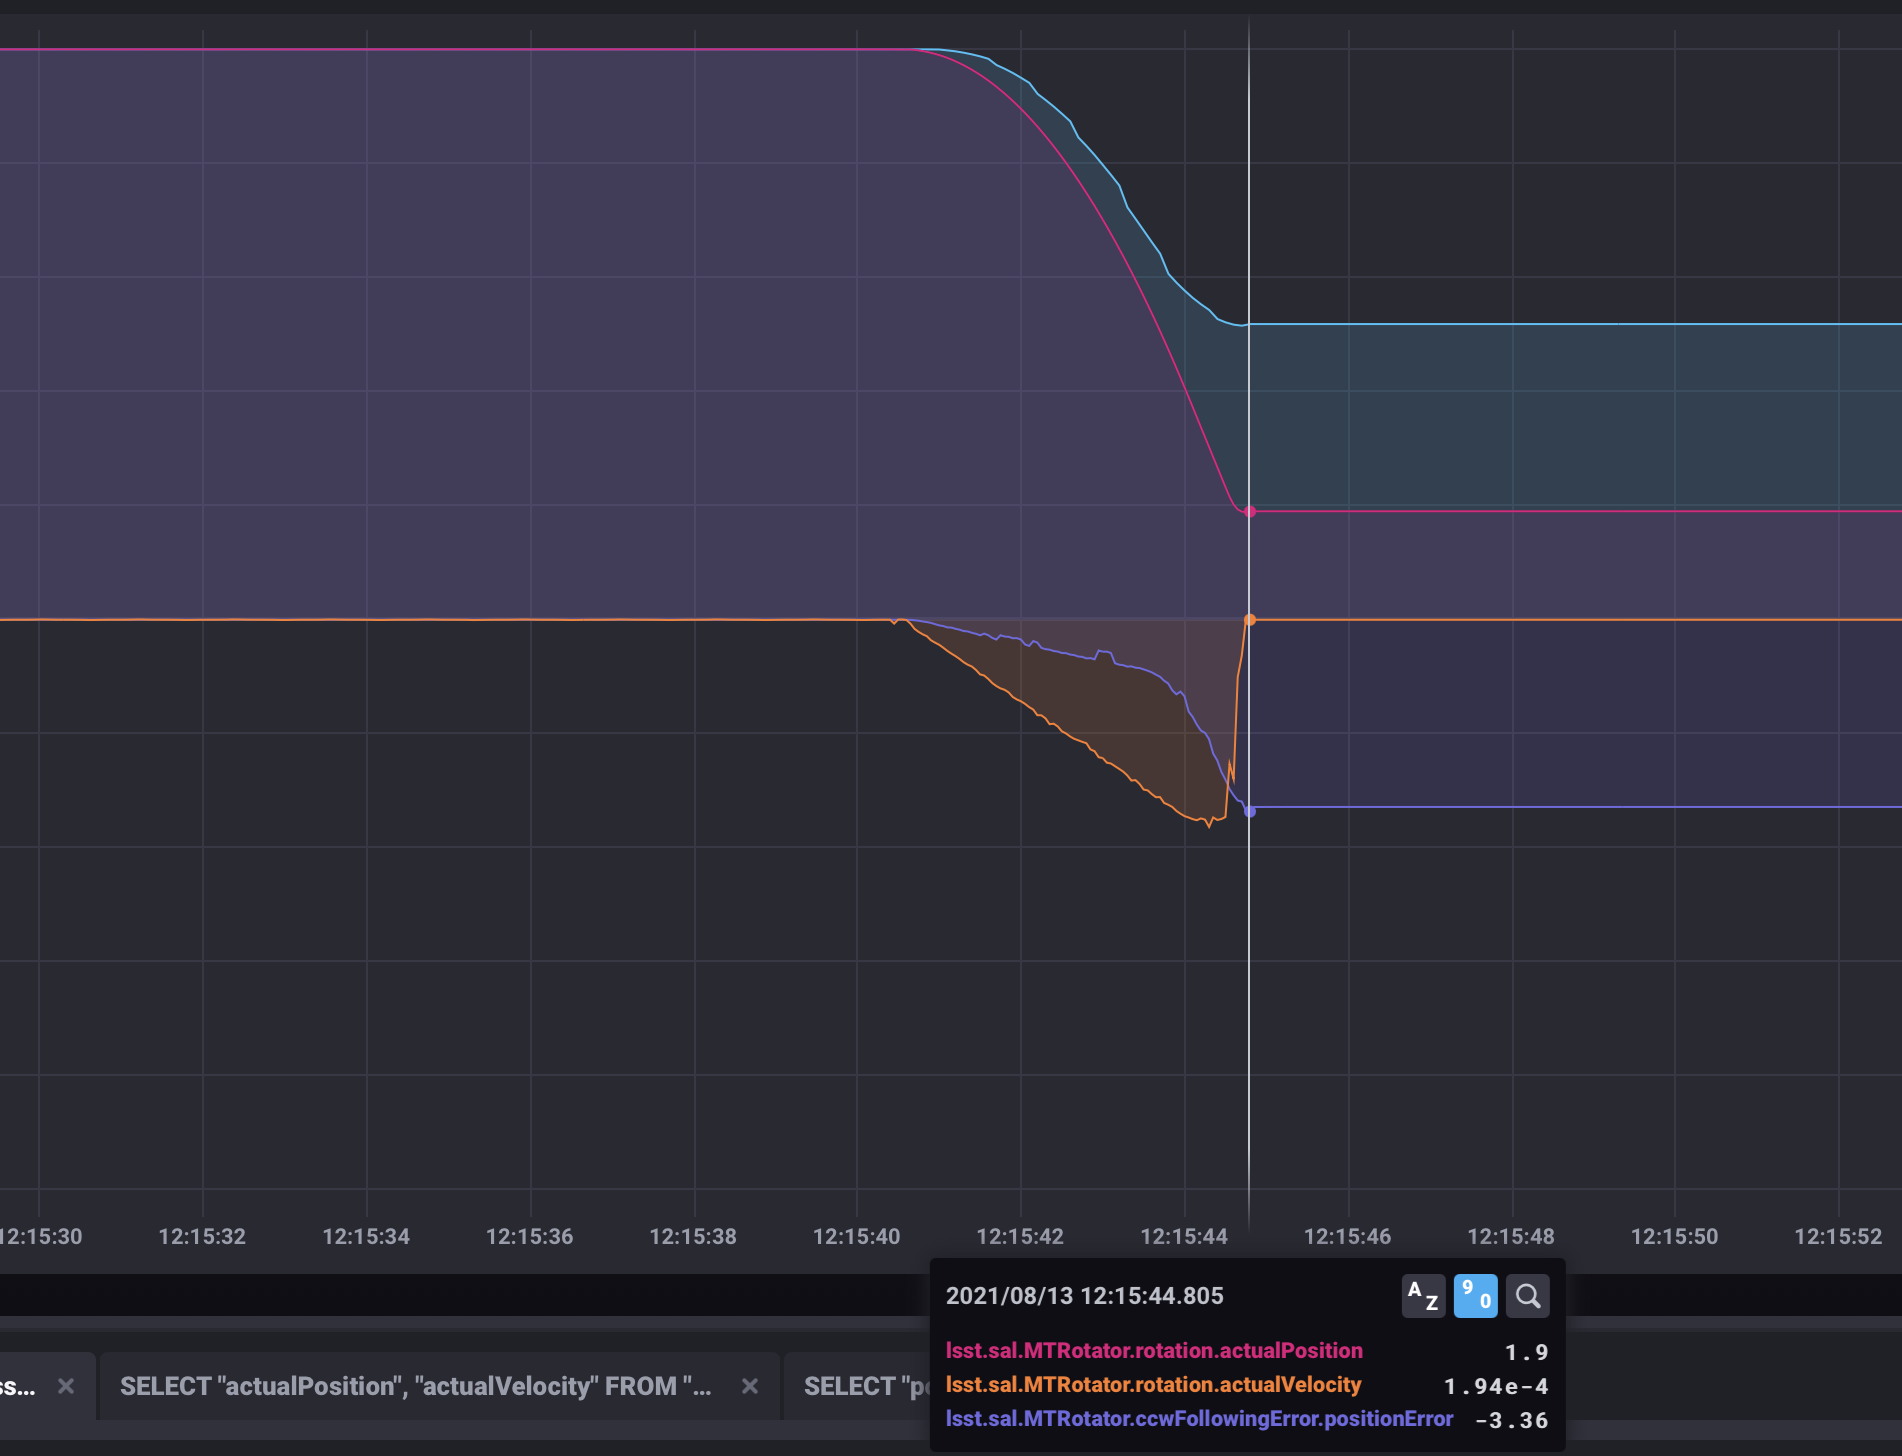
\includegraphics[width=\linewidth]{media/followingFault_2.png}
  \caption{Normal\_Conditions\_RUN\_2}
  \label{fig:Normal_Conditions_RUN_2}
\end{figure}

\begin{figure}
  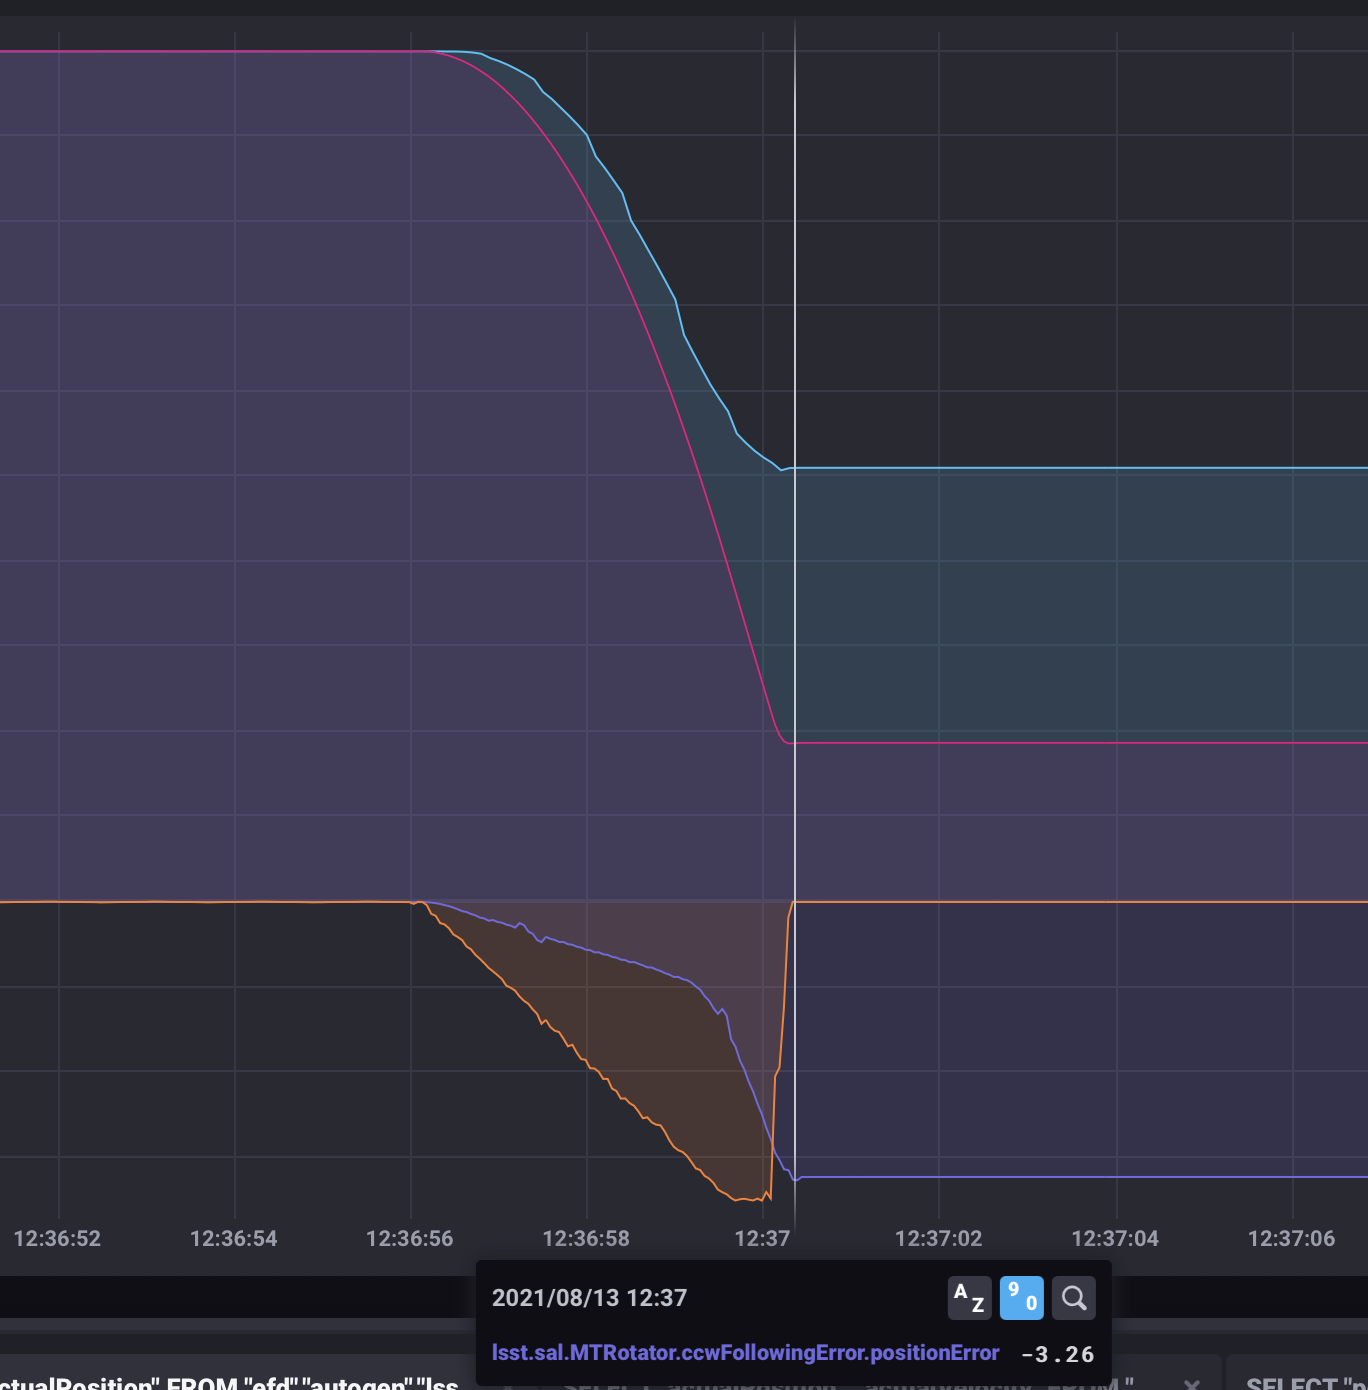
\includegraphics[width=\linewidth]{media/followingFault_3.png}
  \caption{Normal\_Conditions\_RUN\_3}
  \label{fig:Normal_Conditions_RUN_3}
\end{figure}

\begin{figure}
  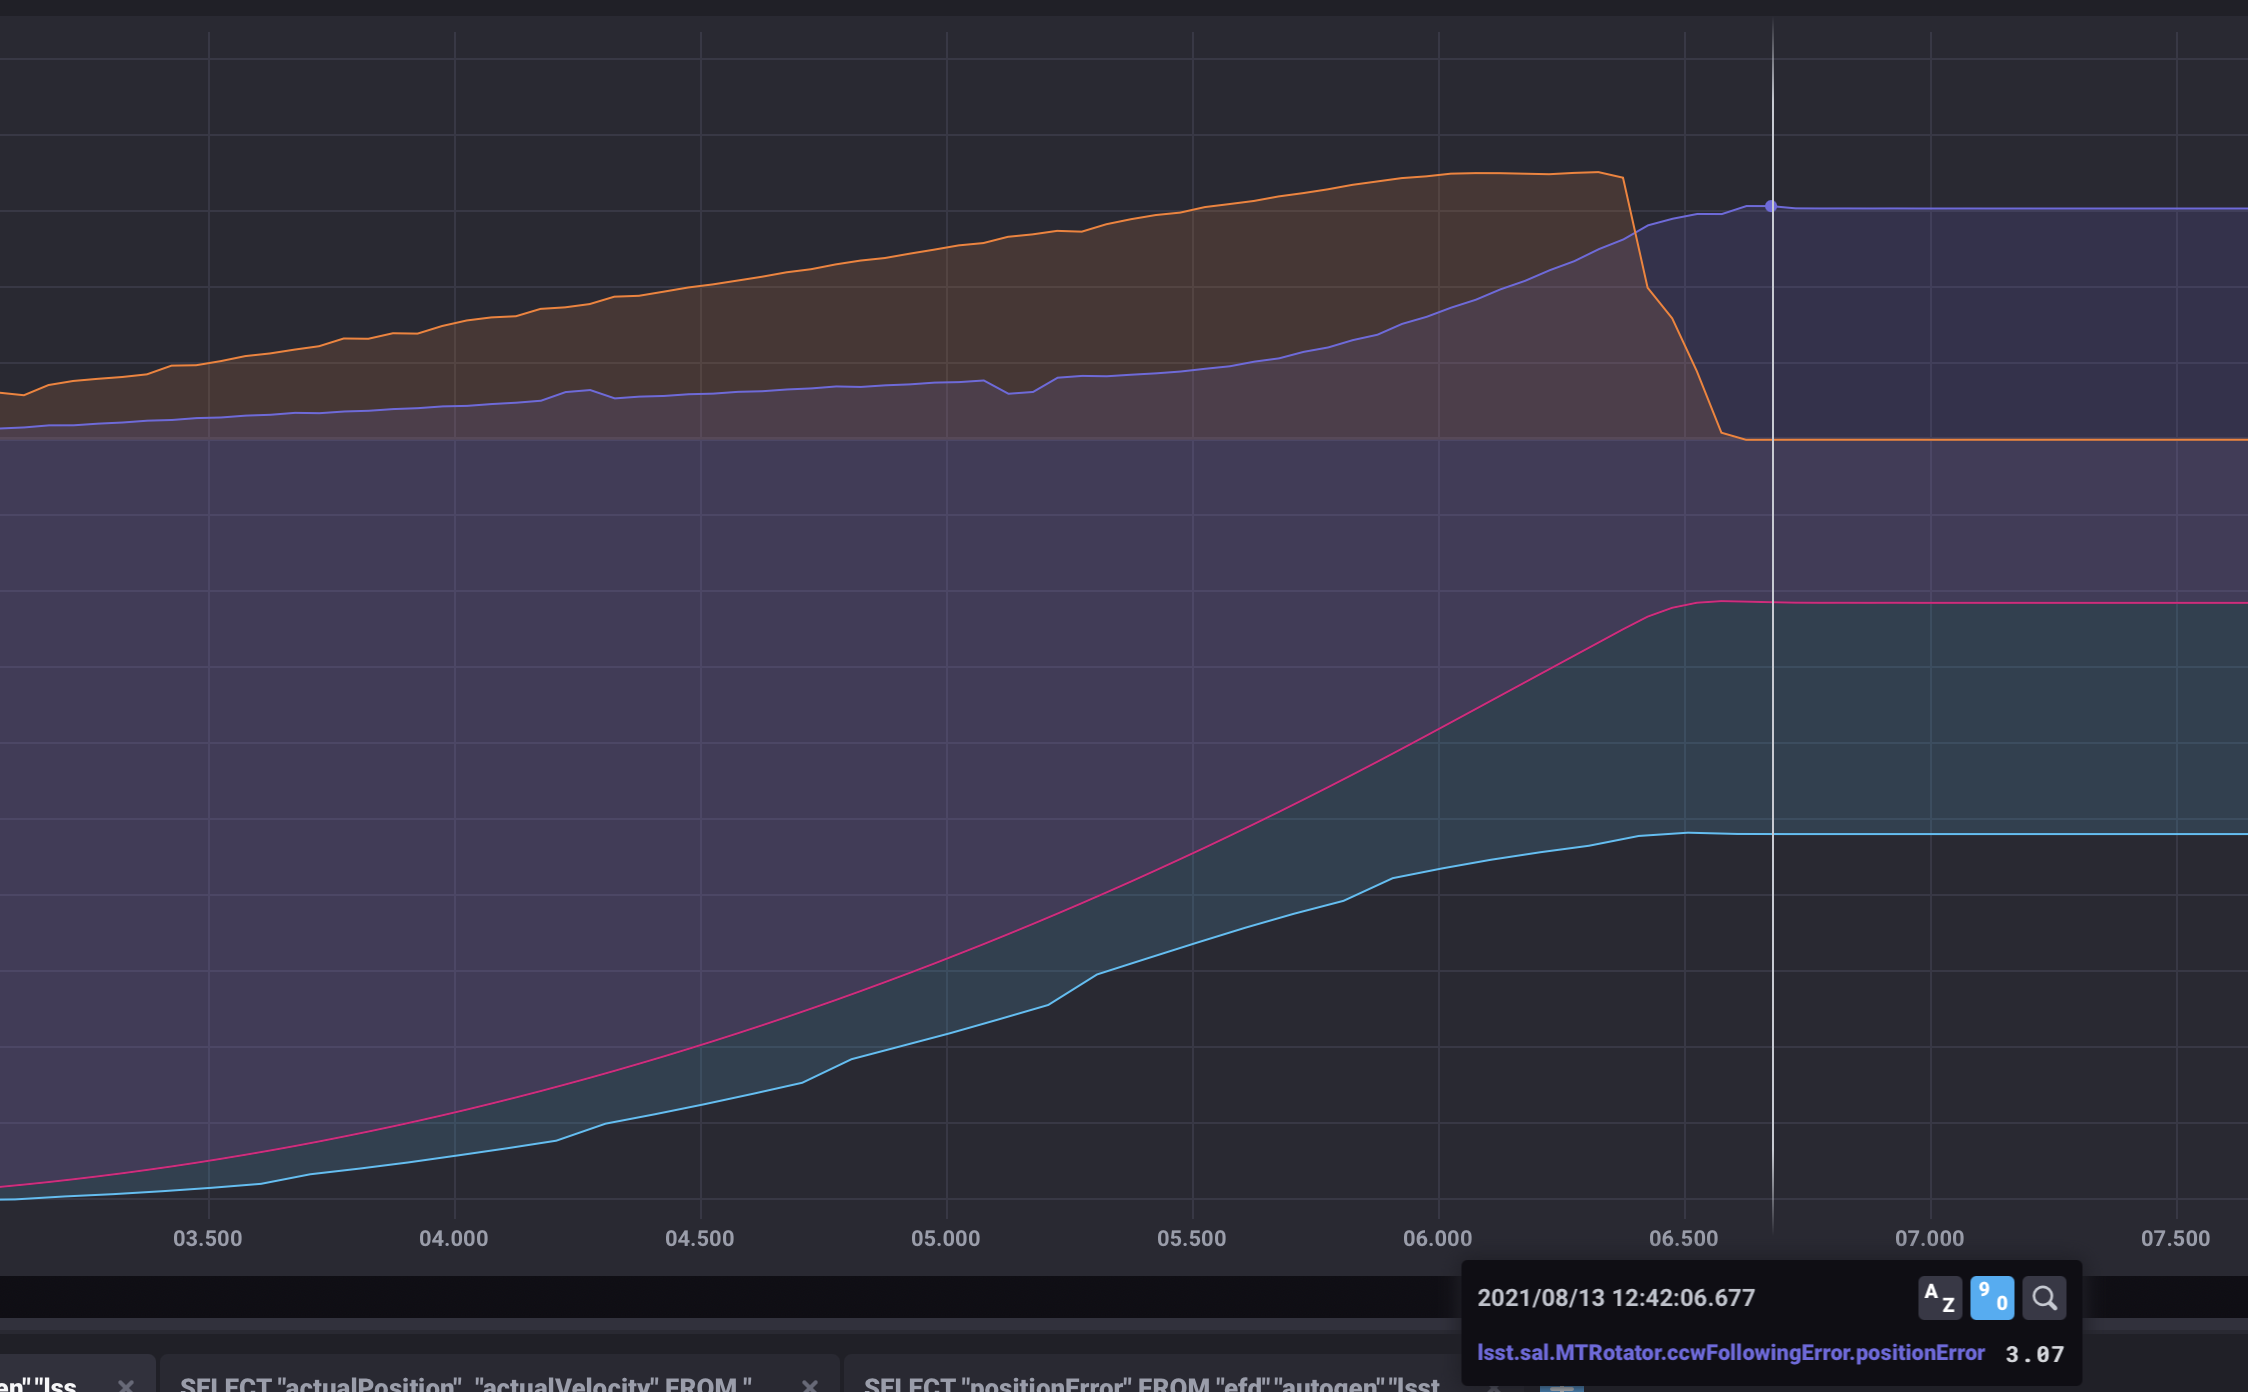
\includegraphics[width=\linewidth]{media/followingFault_4.png}
  \caption{Normal\_Conditions\_RUN\_4}
  \label{fig:Normal_Conditions_RUN_4}
\end{figure}

\begin{figure}
  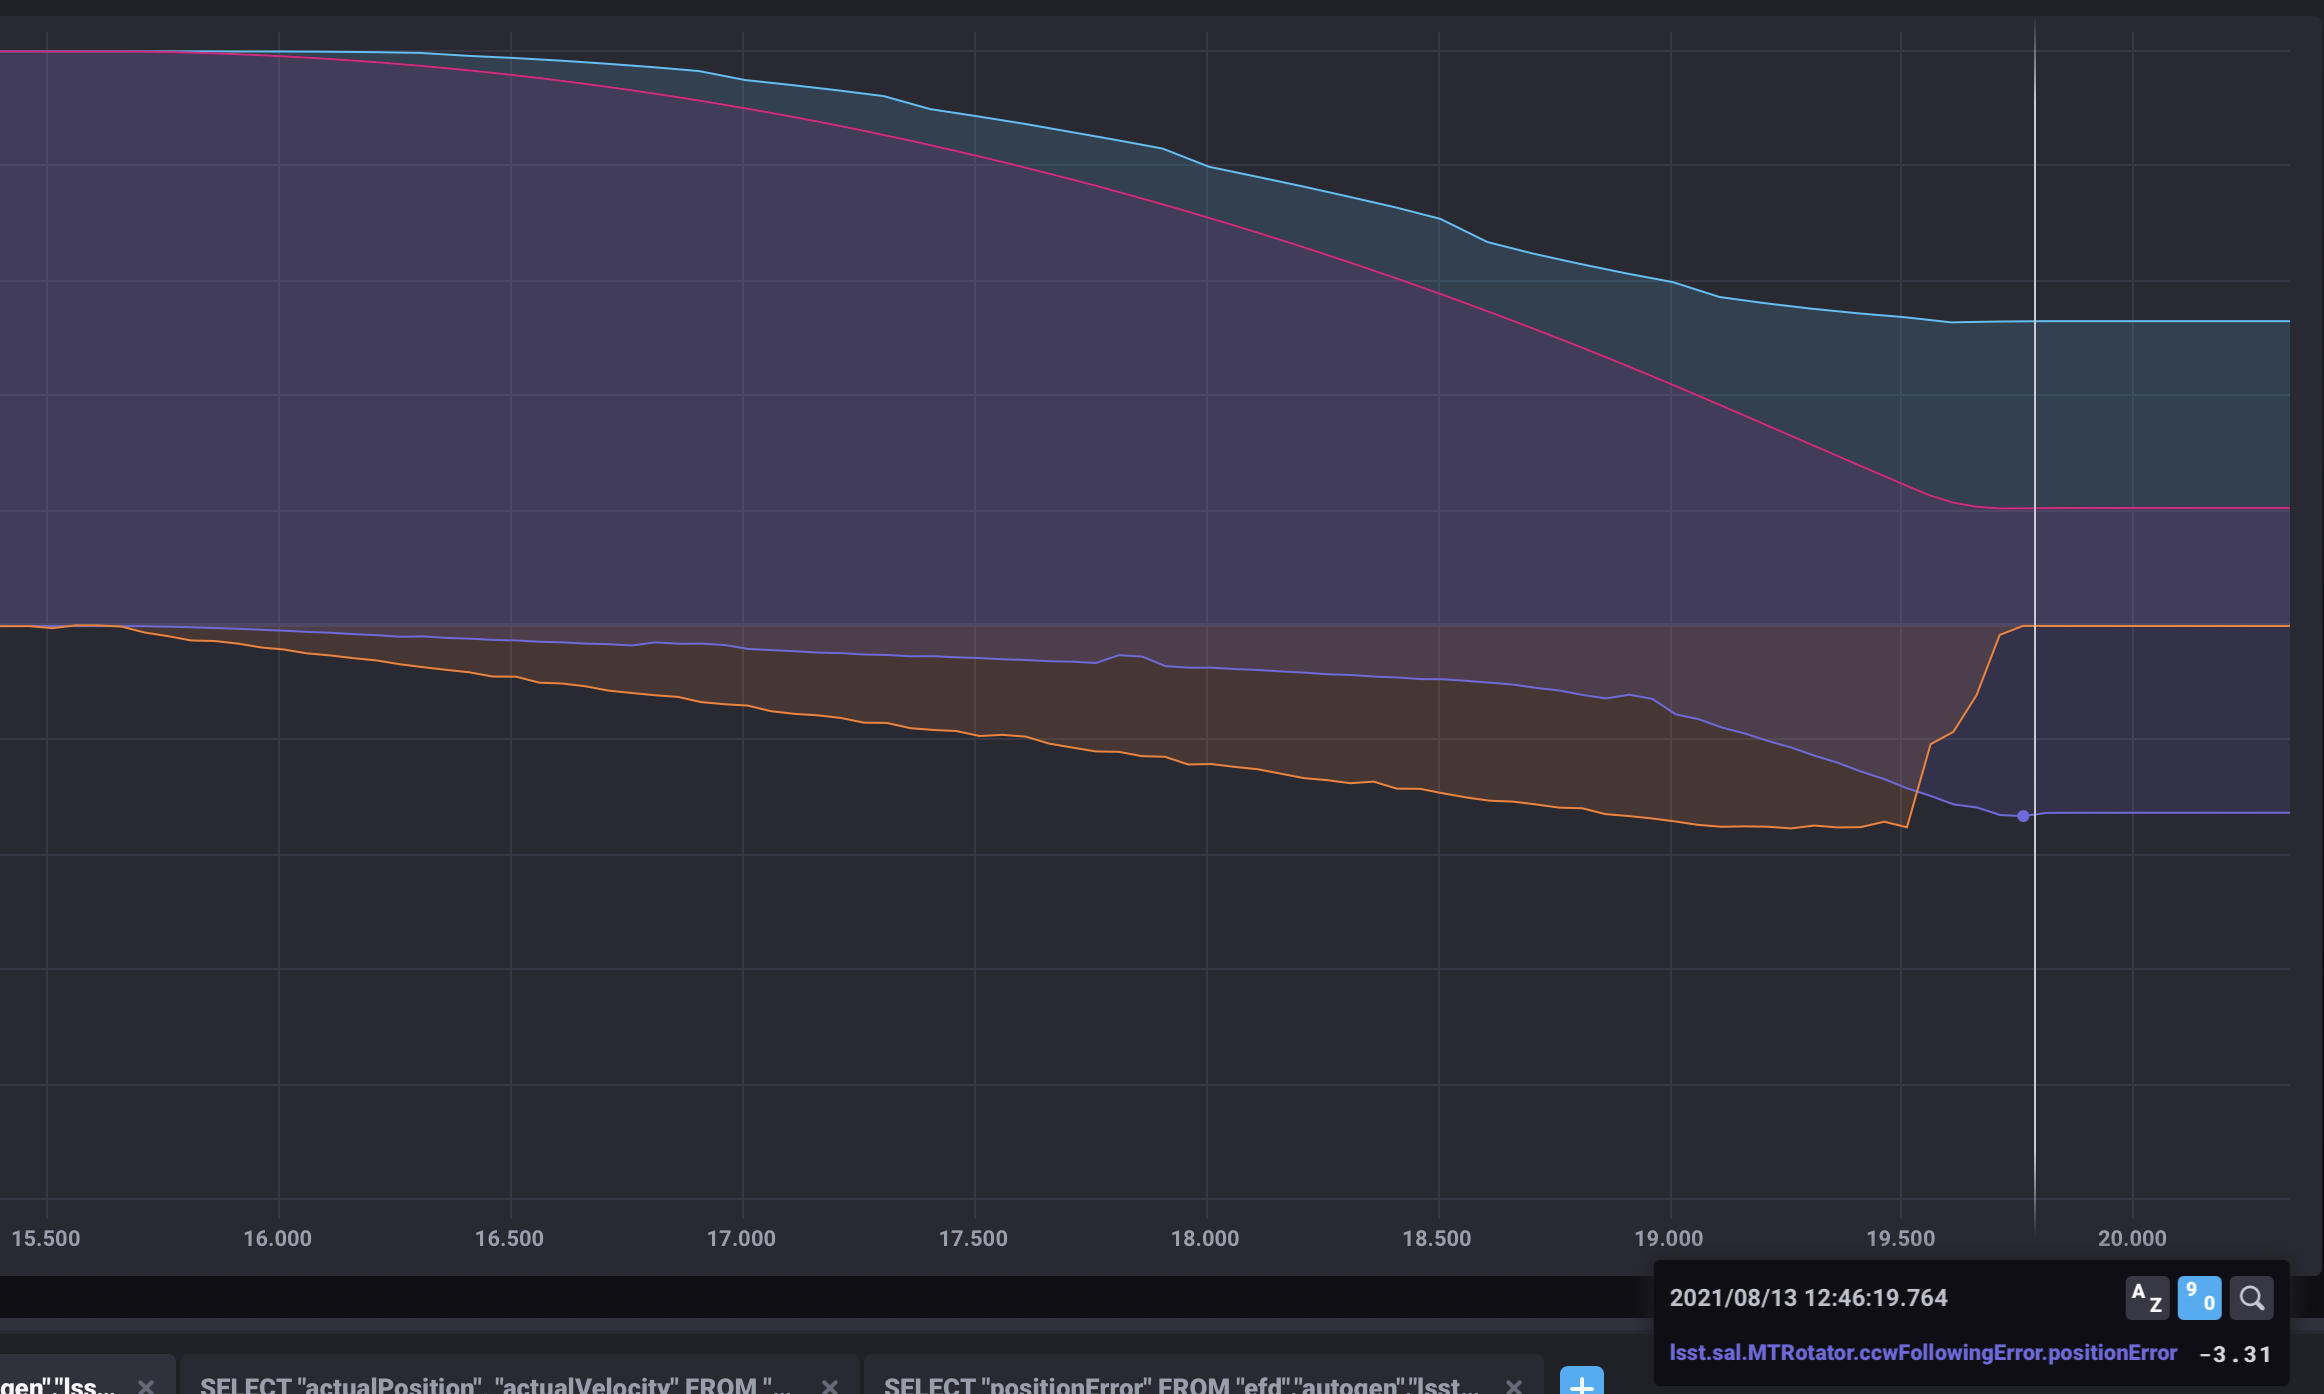
\includegraphics[width=\linewidth]{media/followingFault_5.png}
  \caption{Normal\_Conditions\_RUN\_5}
  \label{fig:Normal_Conditions_RUN_5}
\end{figure}

\end{document}
